\documentclass[10pt,xcolor={dvipsnames}]{beamer}
\usetheme[
%%% option passed to the outer theme
%    progressstyle=fixedCircCnt,   % fixedCircCnt, movingCircCnt (moving is deault)
  ]{Feather}
  
% If you want to change the colors of the various elements in the theme, edit and uncomment the following lines

% Change the bar colors:
\setbeamercolor{Feather}{fg=NavyBlue!20,bg=NavyBlue}

% Change the color of the structural elements:
\setbeamercolor{structure}{fg=NavyBlue}

% Change the frame title text color:
\setbeamercolor{frametitle}{fg=black!5}

% Change the normal text colors:
\setbeamercolor{normal text}{fg=black!75,bg=gray!5}

%% Change the block title colors
\setbeamercolor{block title}{use=Feather,bg=Feather.fg, fg=black!90} 


% Change the logo in the upper right circle:
%\renewcommand{\logofile}{example-grid-100x100pt} 
%% This is an image that comes with the LaTeX installation
% Adjust scale of the logo w.r.t. the circle; default is 0.875
% \renewcommand{\logoscale}{0.55}

% Change the background image on the title and final page.
% It stretches to fill the entire frame!
%\renewcommand{\backgroundfile}{MMCC}

%-------------------------------------------------------
% INCLUDE PACKAGES
%-------------------------------------------------------

\usepackage[utf8]{inputenc}
\usepackage[brazil]{babel}
\usepackage[T1]{fontenc}
% \usepackage{helvet}

%% Load different font packages to use different fonts
%% e.g. using Linux Libertine, Linux Biolinum and Inconsolata
% \usepackage{libertine}
% \usepackage{zi4}

%% e.g. using Carlito and Caladea
\usepackage{carlito}
\usepackage{caladea}
\usepackage{zi4}
\usepackage{amssymb,amsmath,graphicx,charter,latexsym}

\RequirePackage{amsmath} 
\RequirePackage{bbm}
\usepackage{bbm}

\RequirePackage{siunitx}
\usepackage{siunitx}

%%Tables
\usepackage{tabularx,booktabs,dcolumn}

%% Graphics and Subgraphics
\usepackage{subfigure}
\usepackage{graphicx}

\graphicspath{{../newPlots/}}

%%Bibliography
%\setbeamertemplate{bibliography entry title}{}
%\setbeamertemplate{bibliography entry location}{}
%\setbeamertemplate{bibliography entry note}{}

%----------Test Bib Style-------------------------------
\usepackage{natbib}
\bibliographystyle{apalike}
% make bibliography entries smaller
%%\renewcommand\bibfont{\scriptsize}
% If you have more than one page of references, you want to tell beamer
% to put the continuation section label from the second slide onwards
\setbeamertemplate{frametitle continuation}[from second]
% Now get rid of all the colours
\setbeamercolor*{bibliography entry title}{fg=black}
\setbeamercolor*{bibliography entry author}{fg=black}
\setbeamercolor*{bibliography entry location}{fg=black}
\setbeamercolor*{bibliography entry note}{fg=black}
% and kill the abominable icon
\setbeamertemplate{bibliography item}{}
%-------------------------------------------------------

%% e.g. using Venturis ADF Serif and Sans
% \usepackage{venturis}

%-------------------------------------------------------
% DEFFINING AND REDEFINING COMMANDS
%-------------------------------------------------------
%% --
%-------------------------------------------------------
%% Show TOC at every new section
\newif\iflattersubsect

\AtBeginSection[] {
	\begin{frame}<beamer>
		\frametitle{Agenda} %
		\tableofcontents[currentsection]  
	\end{frame}
	\lattersubsectfalse
}

\AtBeginSubsection[] {
	\iflattersubsect
	\begin{frame}<beamer>
		\frametitle{Agenda} %
		\tableofcontents[currentsubsection]  
	\end{frame}
	\fi
	\lattersubsecttrue
}
%% --
%======================================================%
%=========== Informações do documento PDF =============%
%======================================================%
\hypersetup{
	colorlinks = {true},
	linktocpage = {false},
	plainpages = {false},
	linkcolor = {Blue},
	citecolor = {Blue},
	urlcolor = {Red},
	unicode = {true},
	pdftitle ={Teste para Verificação da Hipótese de Ruído Branco utilizando Teoria da Informação},
	pdfauthor = {Marcelo Queiroz de Assis Oliveira},
	pdfsubject = {Disserta\c c\~ao de Mestrado},
	pdfkeywords={Geradores de Números Aleatórios. Testes Teóricos. Testes Estatísticos. Teoria da Informação.},
	pdfcreator = {LaTeX2e},
	pdffitwindow = {false},
	pdfstartview = {FitH},
	pdftoolbar = {true},
	pdfpagemode = {UseOutlines},
	pdfview = {XYZ null null null}
}

%% --
% colored hyperlinks
\newcommand{\chref}[2]{
  \href{#1}{{\usebeamercolor[bg]{Feather}#2}}
}

%-------------------------------------------------------
% INFORMATION IN THE TITLE PAGE
%-------------------------------------------------------

\title[Teste para Verificação da Hipótese de Ruído Branco utilizando Teoria da Informação] % [] is optional - is placed on the bottom of the sidebar on every slide
{ % is placed on the title page
      \textbf{Teste para Verificação da Hipótese de Ruído Branco utilizando Teoria da Informação}
}

\subtitle[]
{
      \textbf{Dissertação de Mestrado}
}

\author[Marcelo Queiroz de Assis Oliveira]
	{{Marcelo Queiroz de Assis Oliveira}\\[1em]
	{\ttfamily marcelo@laccan.ufal.br}\\[1em]}

\institute[]
{
      Universidade Federal de Alagoas\\
      Instituto de Computação\\
      Pós Graduação em Modelagem Computacional de Conhecimento\\
      Laboratório de Computação Científica e Análise Numérica
}

\date{\today}

%-------------------------------------------------------
% THE BODY OF THE PRESENTATION
%-------------------------------------------------------

\begin{document}

%-------------------------------------------------------
% THE TITLEPAGE
%-------------------------------------------------------

{\1% % this is the name of the PDF file for the background
\begin{frame}[plain,noframenumbering] % the plain option removes the header from the title page, noframenumbering removes the numbering of this frame only
  \titlepage % call the title page information from above
\end{frame}}


\begin{frame}{Agenda}{}
\tableofcontents
\end{frame}

%-------------------------------------------------------
\section{Introdução}
%-------------------------------------------------------
\subsection{Números Aleatórios}
%-------------------------------------------------------

\begin{frame}{Introdução}{Números Aleatórios}
	\begin{figure}[hbt]
		\centering
		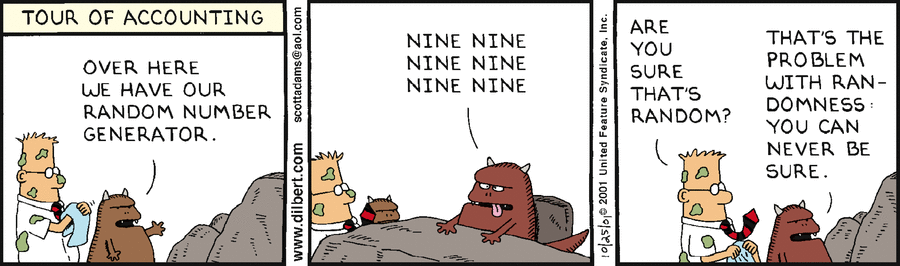
\includegraphics[width=\linewidth]{dilbert}
		\caption{Visão de Dilbert de um gerador de números aleatórios}\label{fig:Dilbert}
	\end{figure}
\end{frame}

\begin{frame}{Introdução}{Números Aleatórios}
Números aleatórios perfazem uma das partes mais importantes em aplicações computacionais nos vários campos do conhecimento, como aborda \cite{Knuth:98}: \pause
\begin{block}{}
\begin{itemize}
\item {\tt Simulação} \pause
\item {\tt Amostragem} \pause
\item {\tt Programação de Computadores} \pause
\item {\tt Tomada de Decisão} \pause
\item {\tt Criptografia} \pause
\item {\tt Estética} \pause
\item {\tt Diversão}
\end{itemize}
\end{block}
\end{frame}

\begin{frame}{Introdução}{GNAs e GNPAs}
	\begin{block}{Geradores de Números Aleatórios - GNAs}
		A maior parte dos geradores utiliza-se de fenômenos físicos naturais como, decaimento radioativo, ruidos termais em semiconcutores, amostras de som num local ruidoso, ruído no espectro eletromagnético, dentre outros que, por óbvia dedução, carecem de algum hardware específico para serem capturados, o que dificulta sua obtenção. 
	\end{block}
\pause
	\begin{block}{Geradores de Números Pseudo-Aleatórios - GNPAs}
		Dadas as dificuldades descritas anteriormente, atualmente a maneira mais conveniente e confiável de se gerar números aleatórios para diversas aplicações é através de algoritmos com um sólido embasamento matemático.
	\end{block}	
	% % % ACF IMPACTO!!! Leve o gerador que compramos
\end{frame}

\begin{frame}{Introdução}{GNAs e GNPAs}
	\begin{figure}[hbt]
		\centering
		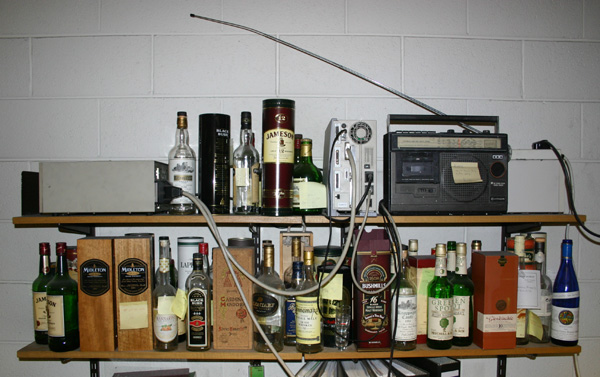
\includegraphics[width=\linewidth]{random_org}
		\caption{Setup do Gerador de Números Aleatórios de www.random.org (1998)}\label{fig:random_org}
	\end{figure}
\end{frame}
%-------------------------------------------------------
\subsection{Testes}
%-------------------------------------------------------
\begin{frame}{Introdução}{Testes}
Existem duas abordagens para testar-se a capacidade de geradores aleatórios ou pseudoaleatórios produzirem sequências ditas aleatórias.
Segundo \cite{LEcuyer:92} são elencados em teóricos e empíricos.
\pause
\begin{block}{Testes teóricos}
	Os testes teóricos são bastante específicos para cada tipo de GNPA, pois analisam o as propriedades das sequências a partir da definição do gerador.
\end{block}
\pause
\begin{block}{Testes empíricos}
	Já os testes empíricos valem-se de técnicas estatísticas objetivando avaliar o quão boas são as sequências produzidas por um determinado gerador.
\end{block}	
\end{frame}

\begin{frame}{Introdução}{Testes}
\pause
% % % ACF Essa pausa cria um slide em branco. É isso que você quer?
\begin{block}{NIST}
	Desde 1997, o Grupo de Trabalho Técnico em Geração de Números Aleatórios (RNG-TWG) tem trabalhado no desenvolvimento de uma bateria de testes estatísticos apropriados para a avaliação de geradores de números aleatórios e pseudoaleatórios utilizados em aplicações criptográficas.
\end{block}
\pause
\begin{block}{Diehard[er]}
	George Marsaglia desenvolveu a bateria de testes Diehard em 1995, e os disponibilizou em CD-ROM.
	Robert Brown identificou limitações nessa bateria de testes, os implementou novamente na linguagem de programação C, acrescentou testes da bateria NIST e disponibilizou um conjunto ampliado de testes denominado Dieharder.
	% % % ACF Sabe a data? Acrescente.
\end{block}	
\end{frame}

\begin{frame}{Introdução}{Testes}
\pause
\begin{block}{ENT}
	ENT \cite{ENTTestSuite} realiza uma variedade de testes no fluxo de bytes de um arquivo (ou na entrada padrão se nenhum arquivo for especificado). É mantido no Fourmilab (\url{http://www.fourmilab.ch/random/}) por John Walker.
\end{block}
\pause
% % % ACF Idem acima
\begin{block}{TestU$01$}
	Considerado como o estado da arte dos testes para geradores de números aleatórios \citep{LEcuyer:07}, o TestU$01$ se apresenta como uma biblioteca de software escrita em $ANSI$ $C$ que oferece uma coleção de utilitários para testagem, ele provê implemetações generalistas dos testes estatísticos clássicos para geradores de números aleatórios, bem como de vários outros propostos na literatura, além de propor alguns originais.
\end{block}	
\end{frame}

\begin{frame}{Introdução}{Testes}
\pause
% % % ACF Idem acima
\begin{block}{Visualização}
	O intuito desses testes é a verificação de que os dados produzidos por um gerador, seja ele algoritmico ou físico, não se afastam significativamente da hipótese de serem eventos de variáveis independentes e identicamente distribuídas segundo uma lei Uniforme no intervalo $(0,1]$.
\pause	
	
	A componente mais difícil é a de verificar a independência, por se tratar de independência coletiva e não apenas aos pares.
\pause
	
	A falta de independência de uma sequência de $N$ pontos pode se manifestar de várias maneiras.
	Uma delas é quando os pontos jazem em subespaços de dimensão menor a $N$, ao invés de preencher o espaço por completo.
\end{block}
\end{frame}

\begin{frame}{Introdução}{Testes}
\begin{block}{Visualização}
	\begin{figure}[hbt]
		\centering
		\subfigure[Primeira perspectiva\label{MTa}]{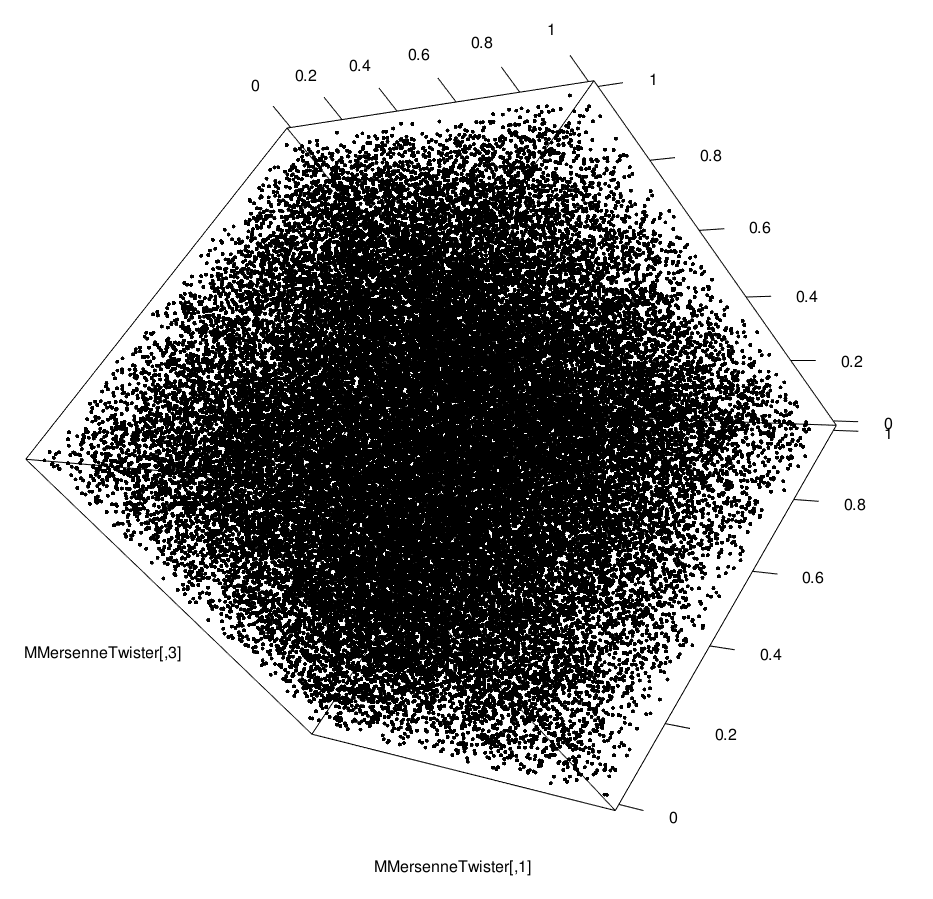
\includegraphics[width=.38\linewidth]{MT3D}}
		\pause
		\subfigure[Segunda perspectiva\label{MTb}]{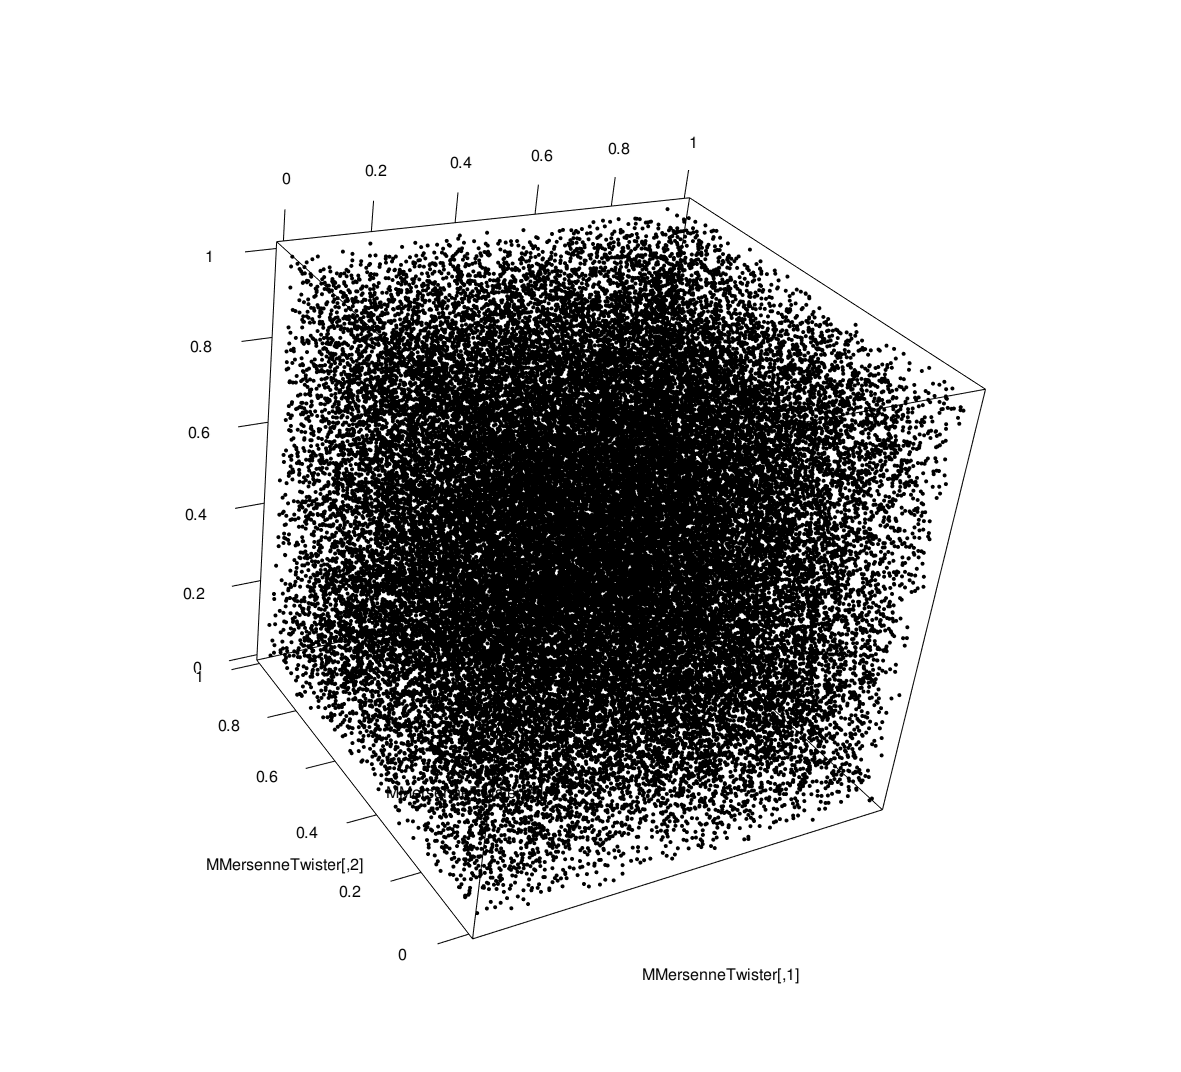
\includegraphics[width=.40\linewidth]{MT3Dsubspace}}
		\caption{Visualização 3D de sequências disjuntas produzidas pelo gerador Mersenne-Twister}\label{fig:3DMT}
	\end{figure}
\end{block}
\end{frame}

\begin{frame}{Introdução}{Testes}
\begin{block}{Visualização}
	\begin{figure}[hbt]
		\centering
		\subfigure[Primeira perspectiva\label{Ra}]{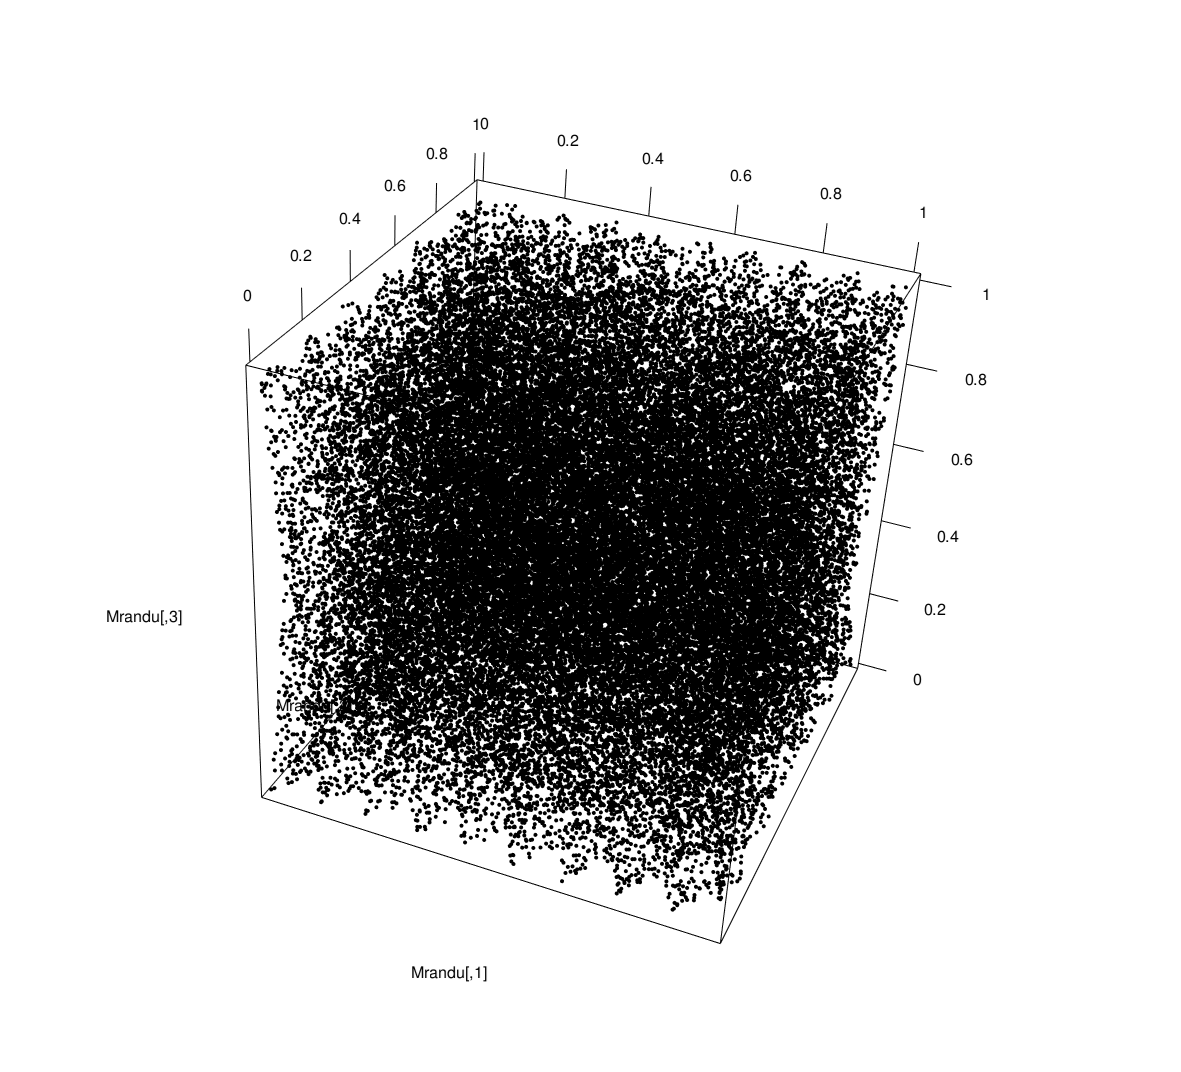
\includegraphics[width=.48\linewidth]{Randu3D}}
		\pause
		\subfigure[Segunda perspectiva\label{Rb}]{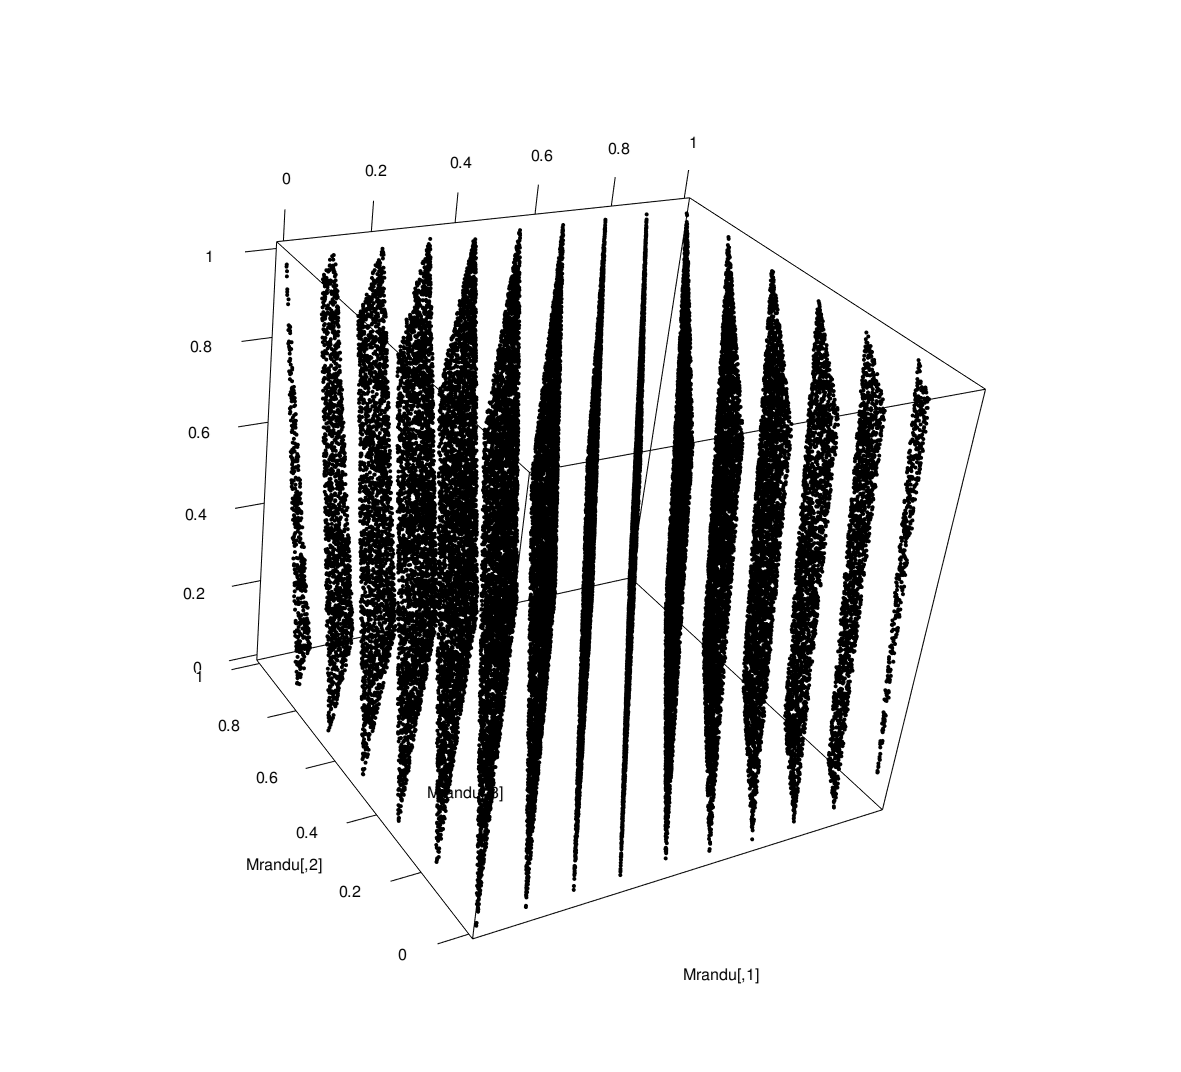
\includegraphics[width=.48\linewidth]{Randu3Dsubspace}}
		\caption{Visualização 3D de sequências disjuntas produzidas pelo gerador RANDU}\label{fig:3DRandu}
	\end{figure}
\end{block}
\end{frame}

%-------------------------------------------------------
\subsection{Descritores baseados em Teoria da Informação}
%-------------------------------------------------------

\begin{frame}{Introdução}{Descritores baseados em Teoria da Informação}

\begin{block}{Descritores baseados em Teoria da Informação}
	\pause

	O trabalho pioneiro de \cite{PermutationEntropyBandtPompe} representa uma mudança de paradigma na análise de séries temporais, e será o nosso marco referencial teórico.
	\pause	
	
	Eles propõem uma técnica não-paramétrica de análise de sequências que consiste em transformar palavras de $D$ dados não necessariamente subsequentes em símbolos ordinais.
	\pause
	
	Esses símbolos codificam a ordem que as $D$ observações têm na sequência e, portanto, são bem menos sucetíveis a contaminação dos que os próprios valores.
\end{block}
\end{frame}

\begin{frame}{Introdução}{Descritores baseados em Teoria da Informação}
\begin{block}{Descritores baseados em Teoria da Informação}
	\pause
	
Forma-se então um histograma de proporções dos símbolos observados, e calculam-se duas quantidades: a Entropia e a Divergência de Jensen-Shannon a uma distribuição de referência (usualmente a uniforme).

	\pause
A série, finalmente, é representada pelo par de valores Entropia-Complexidade Estatística, sendo que esta última é o produto da Entropia e a Divergência de Jensen-Shannon.

	\pause
O conjunto de valores possíveis dos pontos característicos de qualquer série não varre $\mathbbm{R^2}$, mas constitui-se em um subconjunto compacto do plano: o plano Entropia-Complexidade.
\end{block}
\end{frame}

\begin{frame}{Introdução}{Testes}
\begin{block}{Visualização}
	\begin{figure}[hbt]
		\centering
		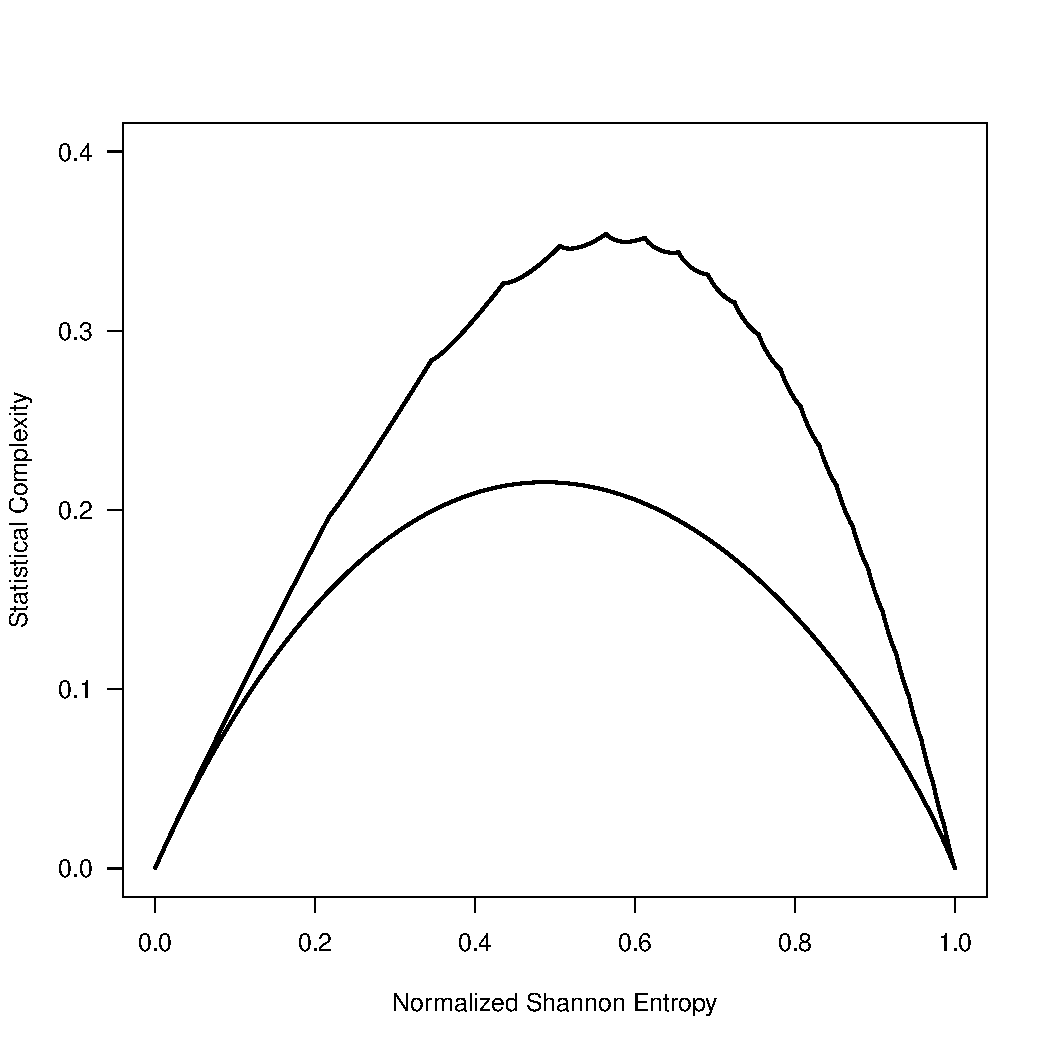
\includegraphics[width=.4\linewidth]{plano_HC}
		\caption{Plano Entropia-Complexidade.}\label{fig:Plano_HC}
	\end{figure}
\end{block}
\end{frame}

\begin{frame}{Introdução}{Descritores baseados em Teoria da Informação}
\begin{block}{Algumas aplicações emblemáticas dessa abordagem:}
\begin{description}
	\item[\cite{RandomNumberGeneratorsCausality}] mostram que o plano Entropia-Complexidade permite prever o resultado dos testes Diehard de qualidade de GNPA.
	\item[\cite{GeneralizedStatisticalComplexityMeasuresGeometricalAnalyticalProperties}] analisam o mapa caótico logístico e discutem cotas no plano Entropia-Complexidade.
	\item[\cite{EEGAnalysisWaveletInformationTools}] analisam dados de eletroencefalogramas de pacientes com epilepsia 	utilizando decomposição wavelet e o plano Entropia-Complexidade.
	\item[\cite{De_Micco_2008}] avaliam melhorias da qualidade de sequências pseudoaleatórias.
	%\item[\cite{De_Micco_2009}] estudam as componentes caóticas de GNPAs.
	\item[\cite{ComplexNetworksEvolution}] analisam a evolução de redes dinâmicas com descritores baseados em Teoria da Informação.
	%\item[\cite{DistinguishingChaoticStochasticDynamicsTimeSeriesMultiscaleSymbolicApproach}] analisam a relação entre dinâmicas caóticas e estocásticas com uma abordagem multiescala.
\end{description}
\end{block}
\end{frame}

\begin{frame}{Introdução}{Descritores baseados em Teoria da Informação}
\begin{block}{Algumas aplicações emblemáticas dessa abordagem:}
	\begin{description}
		\item[\cite{StructuralChangesDataCommunicationWSN}] utilizam descritores de Teoria da Informação para descrever a dinâmica de redes de sensores sem fios.
%		\item[\cite{DistinguishingNoiseFromChaos}] caracterizam sequências com componentes caóticas e estocásticas no plano Entropia-Complexidade.
		\item[\cite{CharacterizationVehicleBehaviorInformationTheory}] analisam o comportamento de veículos em larga escala em função da topologia de diversas cidades.
%		\item[\cite{DiagnosingDynamicsObservedSimulatedEcosystem}] analisam séries temporais de fenômenos ambientais.
%		\item[\cite{InformationTheoryPerspectiveNetworkRobustness}] verificam o efeito de ataques em redes complexas através de descritores no plano Entropia-Complexidade.
		\item[\cite{ClassificationVerificationOnlineHandwrittenSignatures}] mostram a expressividade dos descritores de Teoria da Informação para o problema de classificação e verificação de assinaturas.
		\item[\cite{CharacterizationElectricLoadInformationTheoryQuantifiers}] conseguem caracterizar o tipo de dispositivo elétrico observando o ponto no plano Entropia-Complexidade em que o histórico do seu consumo é mapeado.
	\end{description}
\end{block}
\end{frame}

%-------------------------------------------------------
\subsection{Delimitação do Problema}
%-------------------------------------------------------

\begin{frame}{Introdução}{Delimitação do Problema}
\begin{block}{Delimitação do Problema}
A motivação deste trabalho é o desenvolvimento de um teste baseado em Teoria da Informação para verificar a hipótese de que uma sequência é ruído branco, isto é, formada por observações de variáveis aleatórias independentes e identicamente distribuídas \textit{(vaiid)}.
\pause

Para tanto, trabalharemos com atributos derivados da simbolização de Bandt \& Pompe.
Cada sequência sob análise será transformada em um ponto no plano Entropia-Complexidade, e será medida a sua distância ao ponto característico de sequências ideais.
\pause

Analisaremos, então, a distribuição empírica de uma variedade de situações de interesse para, finalmente, propor regiões de confiança da hipótese nula.
Por fim, analisaremos sequências com o ferramental aqui proposto.
\end{block}
\end{frame}

%-------------------------------------------------------
\section{Proposta}
%-------------------------------------------------------
\subsection{Fundamentação Teórica}
%-------------------------------------------------------

\begin{frame}{Proposta}{Fundamentação Teórica}
	\begin{block}{Simbolização}
		Dada uma série temporal a tempo discreto $ X = {x_t:1\leq t\leq M} $
 
		de comprimento $N$, uma dimensão $D$ e um tempo de atraso (\textit{delay}) $\tau$, o particionamento é efetuado por meio da reorganização do sistema em conjuntos seguindo os passos:
\pause
		\begin{itemize}
			\item \textbf{Composição dos grupos:} Os conjuntos, ou palavras, de comprimento $D$ e \textit{delay} $\tau$ são definidas por um segmento da série: $$ (x_{t+1},x_{t+\tau},\ldots, x_{t+D\tau}).$$ 
			\pause
			\item \textbf{Formação dos padrões:} Cada palavra é então relacionada a um padrão ordinal $\pi_j$ de ordem $D$, isto é, um elemento indexado univocamente por $$ j\in\{1, 2,\ldots, D-1, D\}. $$
		\end{itemize}
\end{block}
\end{frame}

\begin{frame}{Proposta}{Fundamentação Teórica}
\begin{block}{Simbolização}
	Neste trabalho utilizaremos a atribuição lexicográfica, isto é, se os valores da palavra $(x_{t+1},x_{t+\tau},\ldots, x_{t+D\tau})$ são tais que, ordenados, eles têm índices crescentes $b_1,b_2,\dots,b_D$, então o padrão correspondente será $$\pi=b_1b_2\dots b_D$$
	
	Calcula-se, então, o histograma de proporções $$\mathcal{H} =(p_1,\dots,p_{D!})$$ dos padrões observados:	
	\pause

		$$
		p_j = \frac{1}{t-N+1} \# \{
		\text{padrões } \pi_j \text{ observados}
		\}.
		$$
\pause

	O seguinte passo consiste em calcular descritores a partir desse histograma.
\end{block}
\end{frame}

\begin{frame}{Proposta}{Fundamentação Teórica}
\begin{block}{Simbolização}
Os trabalhos já citados utilizam dois descritores: a Entropia de Shannon e a Complexidade Estatística da série.

A Entropia de Shannon é definida como
$$
E(\mathcal H) = -\sum_{j=1}^{D!} p_j \log p_j,
$$

Esta é uma medida da desordem ou imprevisibilidade da lei subjacente a $\mathcal H$.
\pause
A entropia apenas não consegue caracterizar de forma plena a dinâmica que produz a série.
Torna-se interessante, então, o uso de um outro descritor baseado em quão diferente o histograma $\mathcal H$ é de uma lei de probabilidade de referência medida pela distância de Jensen-Shannon:
$$
JS(\mathcal H, \mathcal H_R) = E((\mathcal H+ \mathcal H_R)/2) -\frac{1}{2}(E(\mathcal H) + E(\mathcal H_R)).
$$
A nossa referência será a lei uniforme.
\end{block}
\end{frame}

\begin{frame}{Proposta}{Fundamentação Teórica}
	\begin{block}{Regiões de confiança no plano Entropia-Complexidade}
	Não conhecemos, contudo, a distribuição conjunta do par $(E,JS)$ para uma sequência de variáveis aleatórias coletivamente independente e identicamente distribuídas segundo uma lei uniforme.
	Como também não conhecemos a distribuição do par $(H,C)$ decidimos fazer a análise empírica de dados obtidos de fontes ``confiáveis''.
	\pause
	
	Para isso, utilizamos três fontes de dados: duas físicas e uma algorítmica.
	As fontes físicas foram dados de medidas de estados quânticos \cite{RNGVacuumStates} (que denominaremos \textit{sequências quânticas}) e de sinais de rádio \cite{RandomHostingAdvice} (que chamaremos \textit{sequências de rádio}).
	A fonte algorítmica é o gerador Mersenne-Twister \citep{Matsumoto98}, considerado um padrão de qualidade de algoritmos de geração de números pseudoaleatórios.
	\end{block}
\end{frame}

\begin{frame}{Proposta}{Fundamentação Teórica}
	\begin{block}{Regiões de confiança no plano Entropia-Complexidade}
	Obtivemos com os autores \num{54000000} de observações de cada gerador físico, e as submetemos à análise dos padrões de Bandt \& Pompe.
	
	Obtivemos os valores de entropia e complexidade estatística para todas as sequências possíveis de tamanho \num{18000}, palavras de tamanho $D\in\{3, 4, 5, 6\}$ e \textit{lag} $\tau\in\{1, 10, 30,50\}$.
	
	Seguindo a proposta de \cite{NewPermutationEntropy}, nossa medida de qualidade é a distância do ponto padrão observado $(E,C)$ no plano Entropia-Complexidade ao ponto ideal $(1,0)$.
	Empregamos, como esse autor, a distância euclidiana.
	\end{block}
\end{frame}
%-------------------------------------------------------     
\section{Resultados}
%-------------------------------------------------------
%-------------------------------------------------------
\subsection{Análise global das sequências}
%-------------------------------------------------------
\begin{frame}{Resultados}{Análise global das sequências}
  \begin{block}{Análise global das sequências}
	Trabalhamos com sequências de observações provindas de três geradores: dois físicos (considerados ``verdadeiramente aleatórios'') e um algorítmico (o gerador Mersenne-Twister, que é reputado um dos melhores geradores pseudoaleatórios).
	\pause
	
	Para cada gerador considerado coletamos sequências disjuntas de tamanho \num{1.000} e \num{50.000}, de cada tamanho de palavra $D$ e a cada \textit{lag} $\tau$.
	Temos, assim, quatro fatores a serem analisados.
	\pause
	
	Cada sequência passou pelo processo de simbolização, e foi calculado o histograma dos símbolos.
	Foram então calculados os valores de Entropia e de Complexidade de cada histograma, bem como a distância euclidiana desses valores ao ponto de referência $(1,0)$.
  \end{block}
\end{frame}

\begin{frame}{Resultados}{Análise global das sequências}
\begin{block}{Sequências quânticas com $1.000$ observações}
	\begin{figure}[hbt]
		\centering
		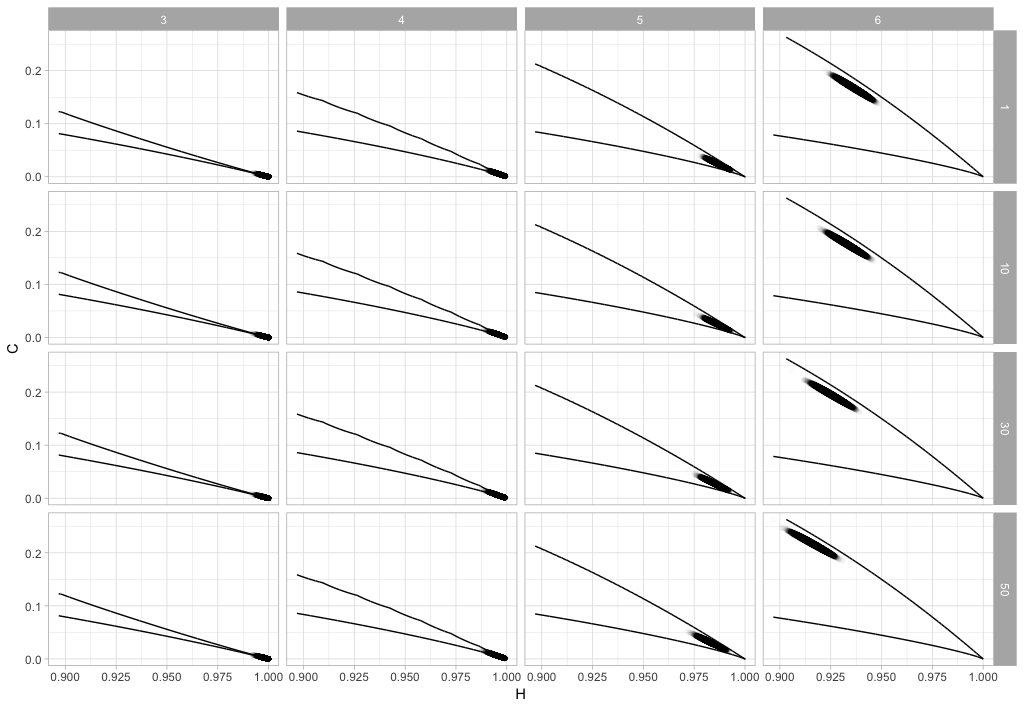
\includegraphics[width=.65\linewidth]{ScatterAll_Quant_1k}
		\caption{Diagramas de dispersão das sequências quânticas com $1.000$ observações para $D\in\{3, 4, 5, 6\}$ (colunas) e $\tau\in\{1, 10, 30, 50\}$ (linhas), com curvas de complexidade mínima e máxima no plano Entropia-Complexidade.}\label{Fig:ScatterAll_Quant_1k}
	\end{figure}
\end{block}
\end{frame}

\begin{frame}{Resultados}{Análise global das sequências}
\begin{block}{Sequências quânticas com $50.000$ observações}
	\begin{figure}[hbt]
		\centering
		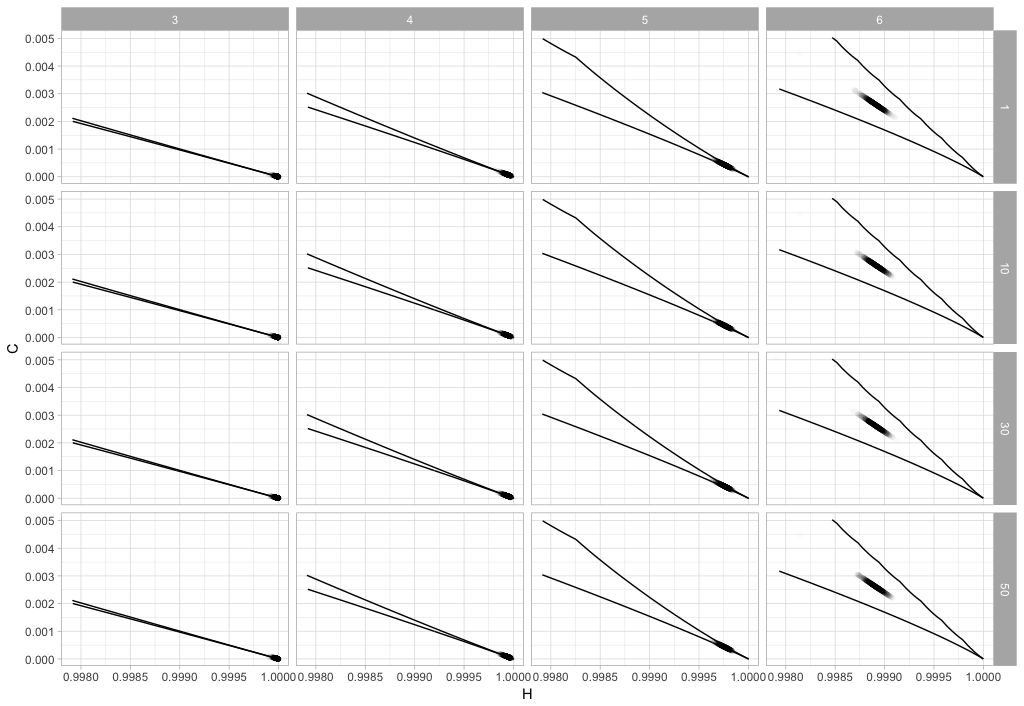
\includegraphics[width=.65\linewidth]{ScatterAll_Quant_50k}
		\caption{Diagramas de dispersão das sequências quânticas com $50.000$ observações para $D\in\{3, 4, 5, 6\}$ (colunas) e $\tau\in\{1, 10, 30, 50\}$ (linhas), com curvas de complexidade mínima e máxima no plano Entropia-Complexidade.}\label{Fig:ScatterAll_Quant_50k}
	\end{figure}
\end{block}
\end{frame}

\begin{frame}{Resultados}{Análise global das sequências}
\begin{block}{Sequências de rádio com $1.000$ observações}
	\begin{figure}[hbt]
		\centering
		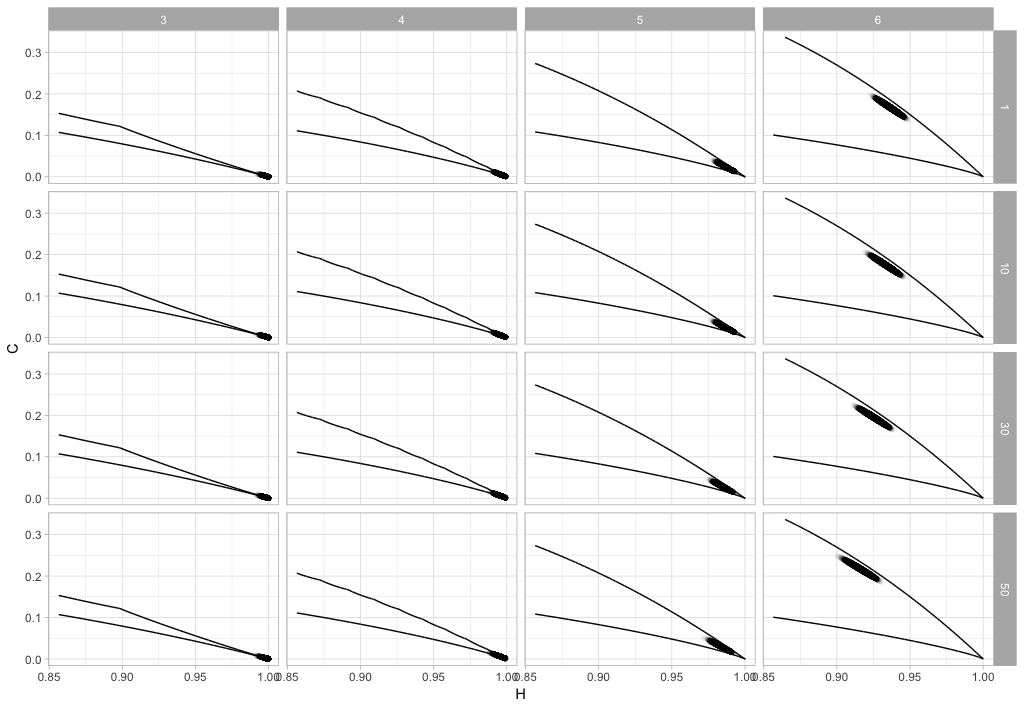
\includegraphics[width=.65\linewidth]{ScatterAll_Radio_1k}
		\caption{Diagramas de dispersão das sequências de rádio com $1.000$ observações para $D\in\{3, 4, 5, 6\}$ (colunas) e $\tau\in\{1, 10, 30, 50\}$ (linhas), com curvas de complexidade mínima e máxima no plano Entropia-Complexidade.}\label{Fig:ScatterAll_Radio_1k}
	\end{figure}	
\end{block}
\end{frame}

\begin{frame}{Resultados}{Análise global das sequências}
\begin{block}{Sequências de rádio com $50.000$ observações}
	\begin{figure}[hbt]
		\centering
		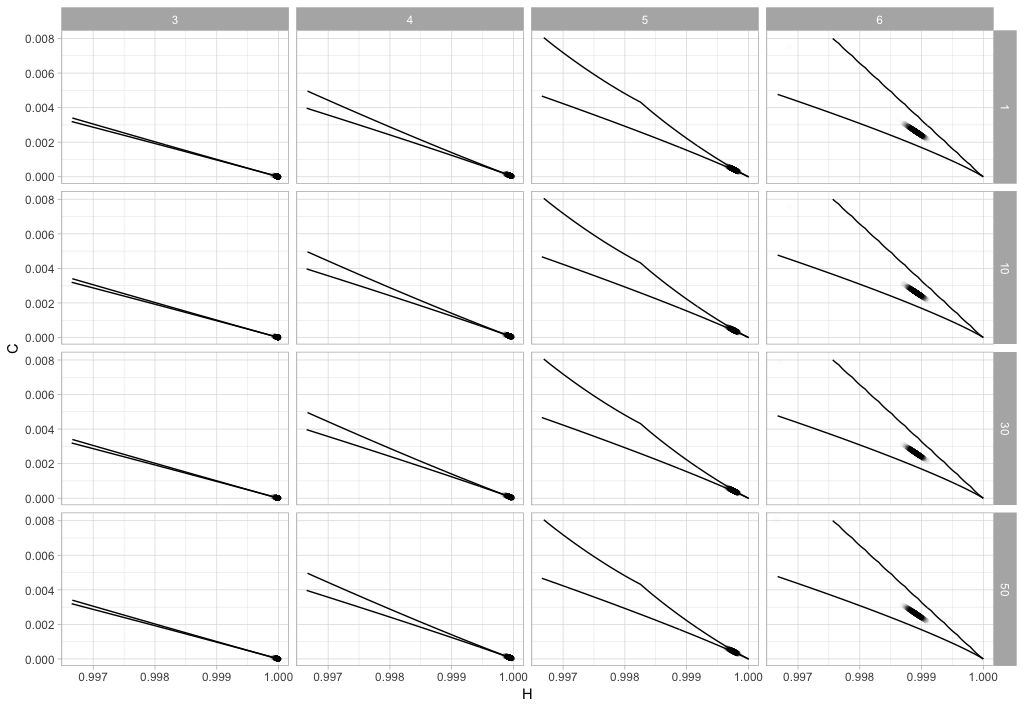
\includegraphics[width=.65\linewidth]{ScatterAll_Radio_50k}
		\caption{Diagramas de dispersão das sequências de rádio com $50.000$ observações para $D\in\{3, 4, 5, 6\}$ (colunas) e $\tau\in\{1, 10, 30, 50\}$ (linhas), com curvas de complexidade mínima e máxima no plano Entropia-Complexidade.}\label{Fig:ScatterAll_Radio_50k}
	\end{figure}	
\end{block}
\end{frame}

\begin{frame}{Resultados}{Análise global das sequências}
\begin{block}{Sequências de Mersenne-Twister com $1.000$ observações}
	\begin{figure}[hbt]
		\centering
		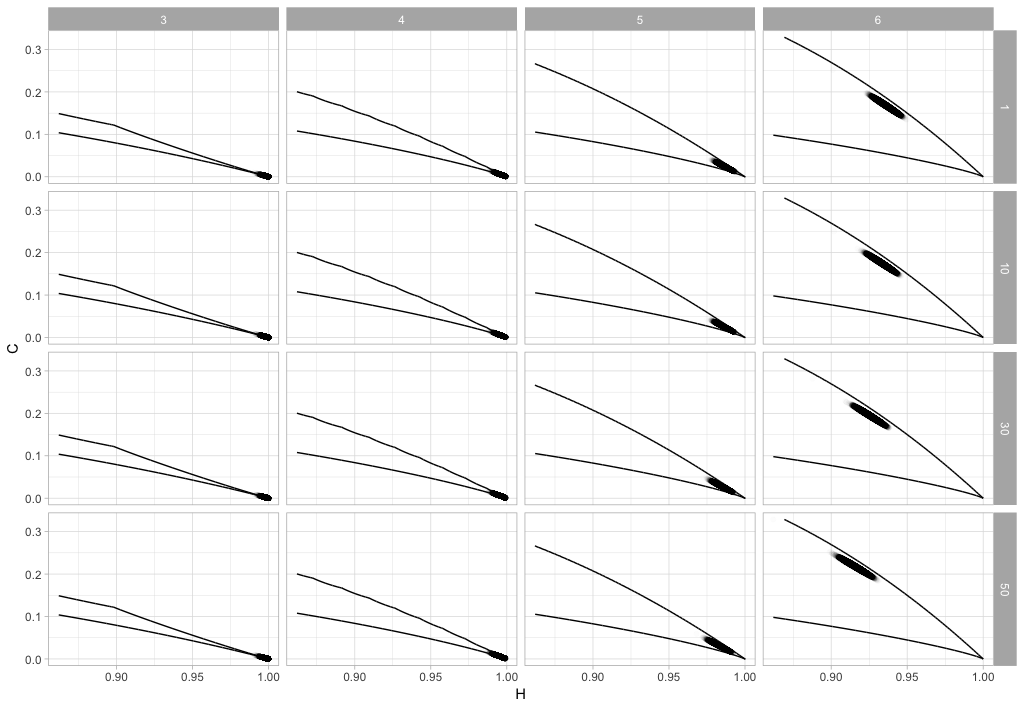
\includegraphics[width=.65\linewidth]{ScatterAll_MT_1k}
		\caption{Diagramas de dispersão das sequências de Mersenne-Twister com $1.000$ observações para $D\in\{3, 4, 5, 6\}$ (colunas) e $\tau\in\{1, 10, 30, 50\}$ (linhas), com curvas de complexidade mínima e máxima no plano Entropia-Complexidade.}\label{Fig:ScatterAll_MT_1k}
	\end{figure}
\end{block}
\end{frame}

\begin{frame}{Resultados}{Análise global das sequências}
\begin{block}{Sequências de Mersenne-Twister com $50.000$ observações}
	\begin{figure}[hbt]
		\centering
		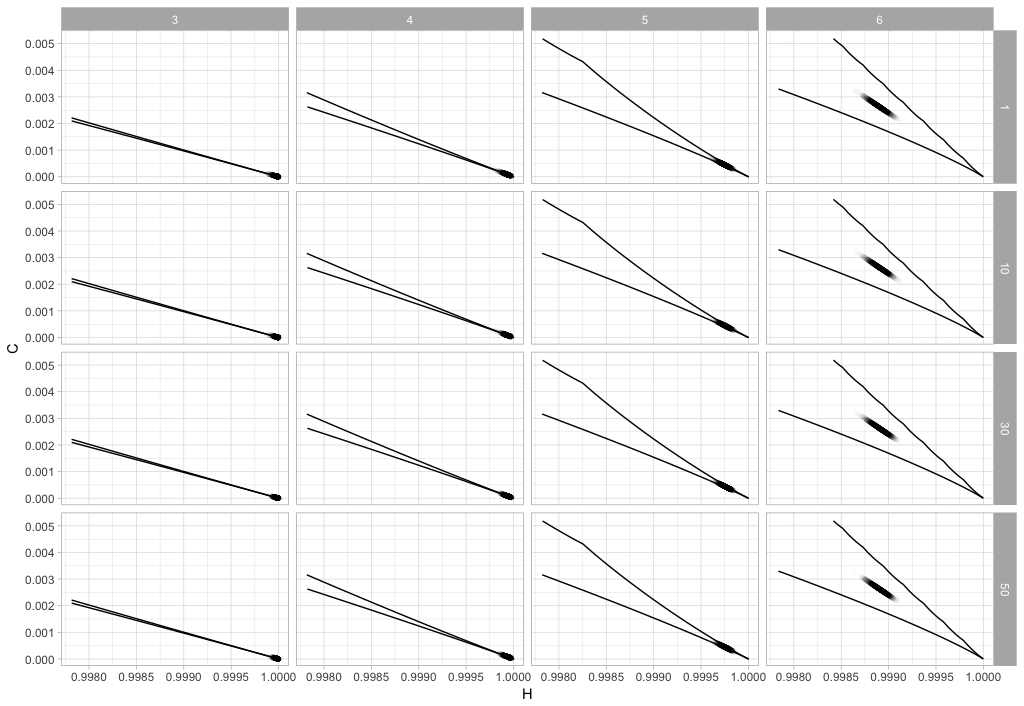
\includegraphics[width=.65\linewidth]{ScatterAll_MT_50k}
		\caption{Diagramas de dispersão das sequências de Mersenne-Twister com $50.000$ observações para $D\in\{3,4,5,6\}$ (colunas) e $\tau\in\{1,10,30,50\}$ (linhas), com curvas de complexidade mínima e máxima no plano Entropia-Complexidade.}\label{Fig:ScatterAll_MT_50k}
	\end{figure}
\end{block}
\end{frame}

%-------------------------------------------------------
\subsection{Histogramas suavizados}
%-------------------------------------------------------
\begin{frame}{Resultados}{Histogramas suavizados}
\begin{block}{}
	A olho nu, $D$ é um fator relevante pois os diagramas de dispersão mostram comportamentos que merecem uma análise mais aprofundada, por outro lado não temos certeza de como $\tau$ e o gerador influenciam os resultados. 
\pause
	\begin{figure} %D=6 %N 1000 t1 t 50
		\centering
		\subfigure[$D=6, \tau=1$]{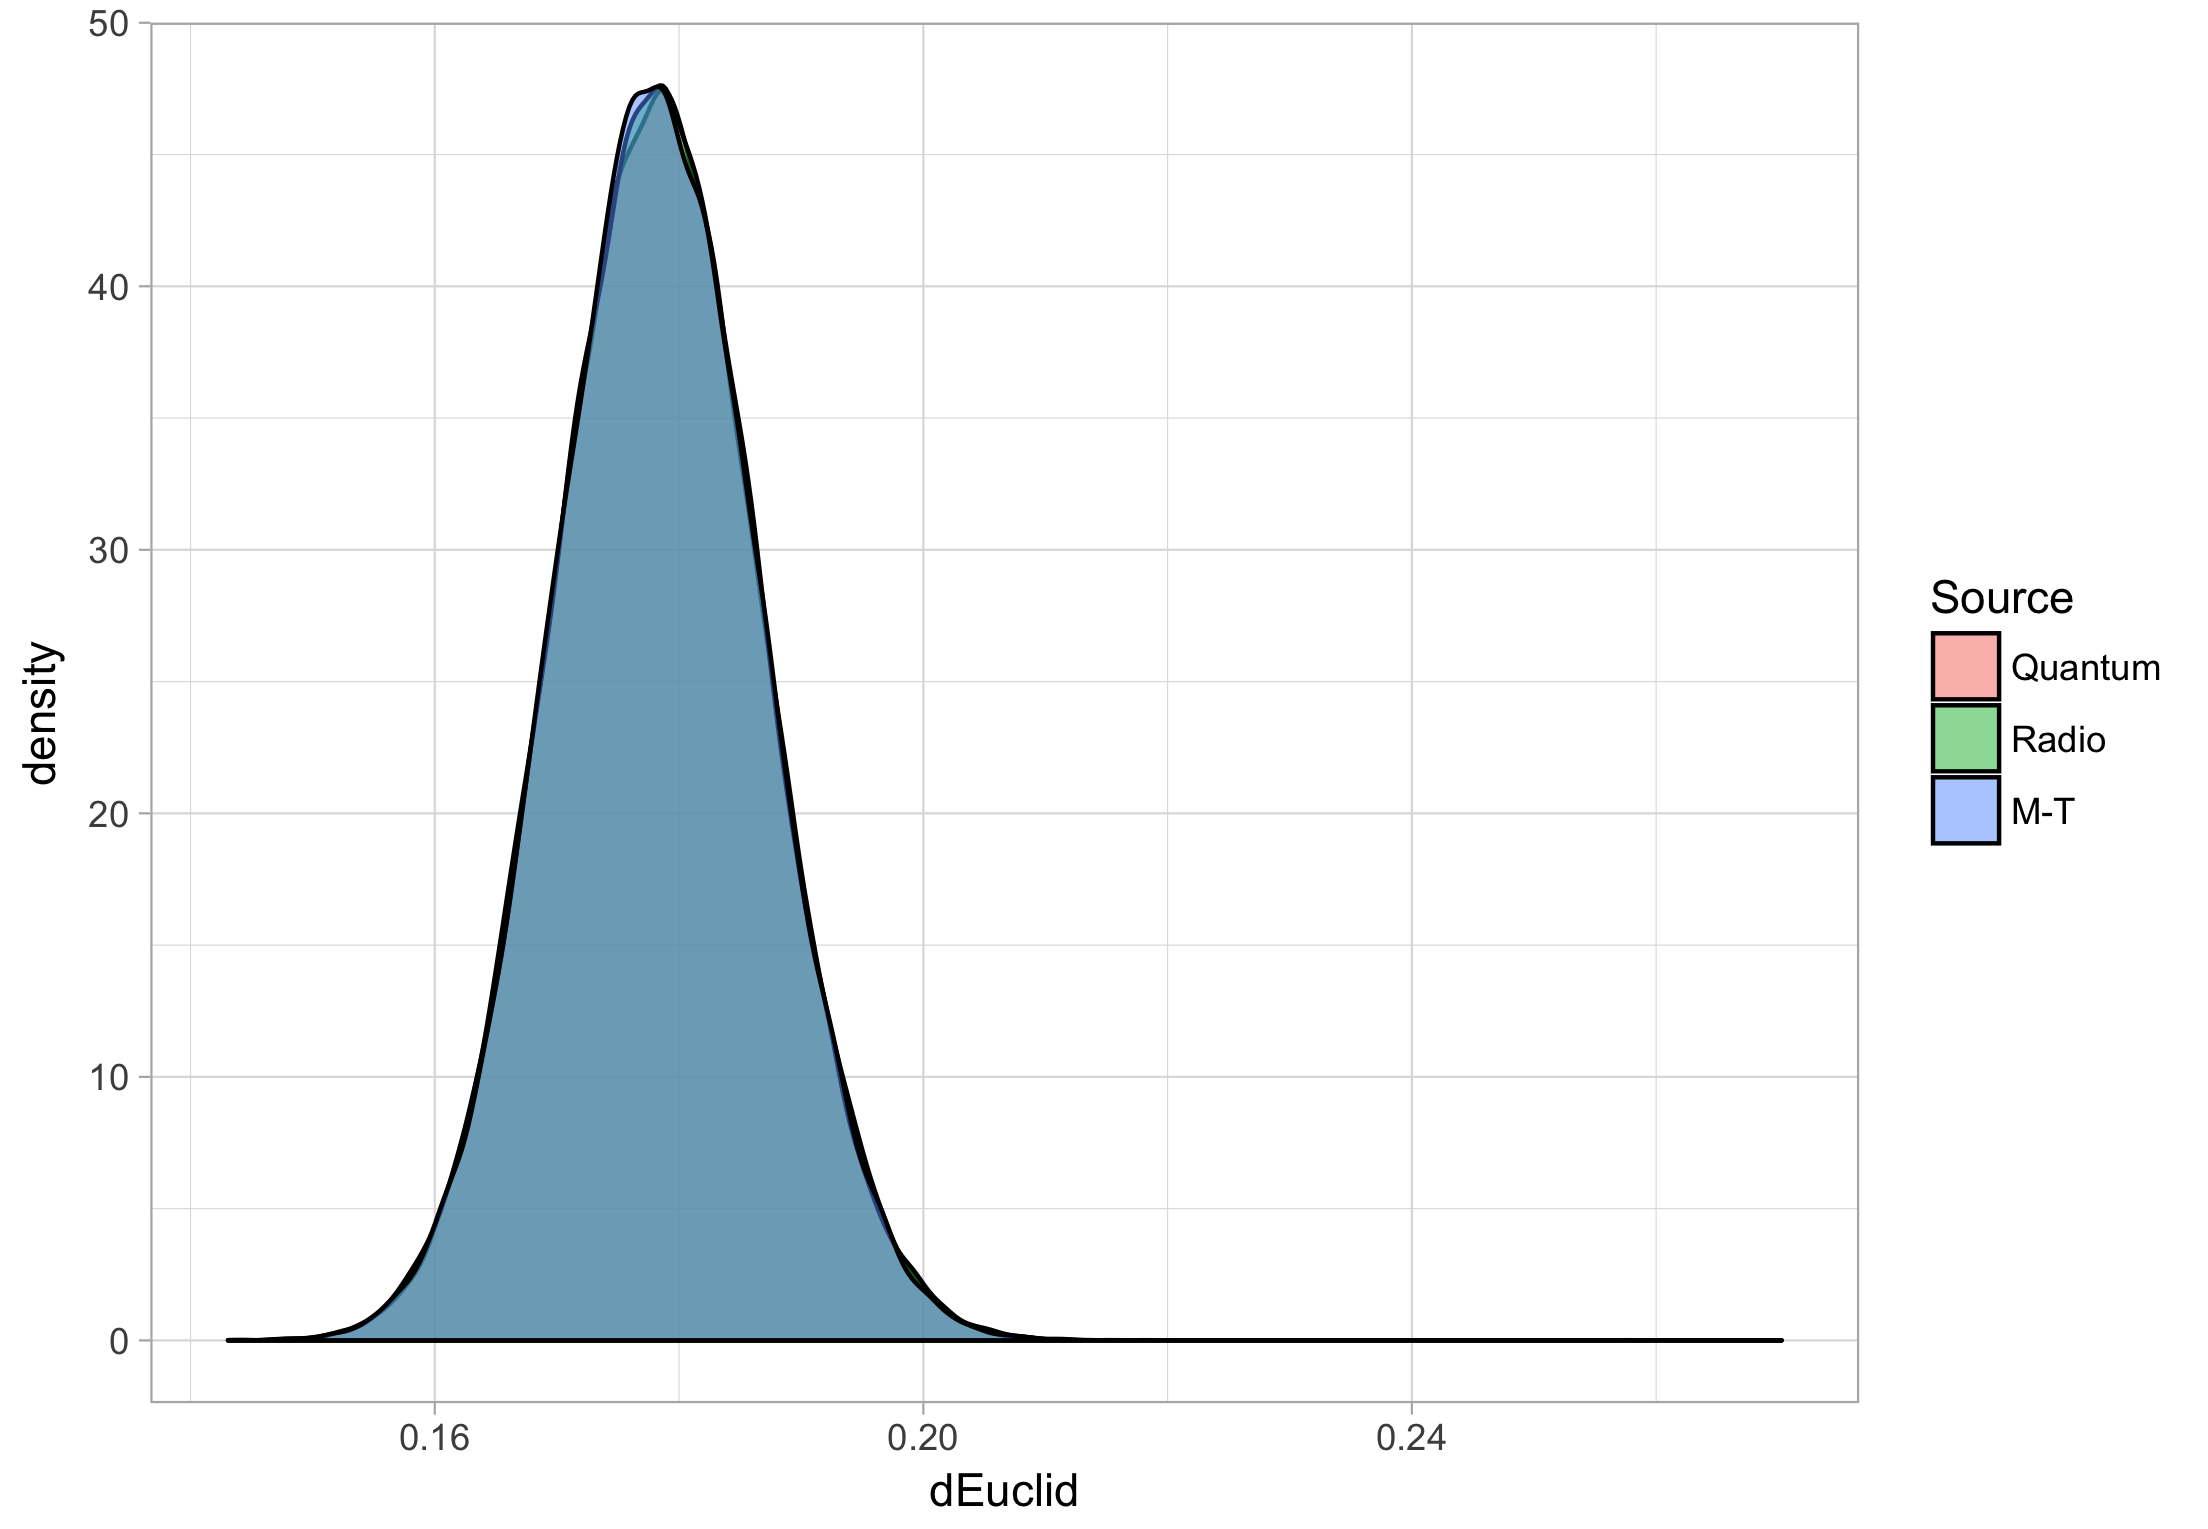
\includegraphics[width=.48\linewidth]{Hist_D6_1k_t1}}
		\subfigure[$D=6, \tau=50$]{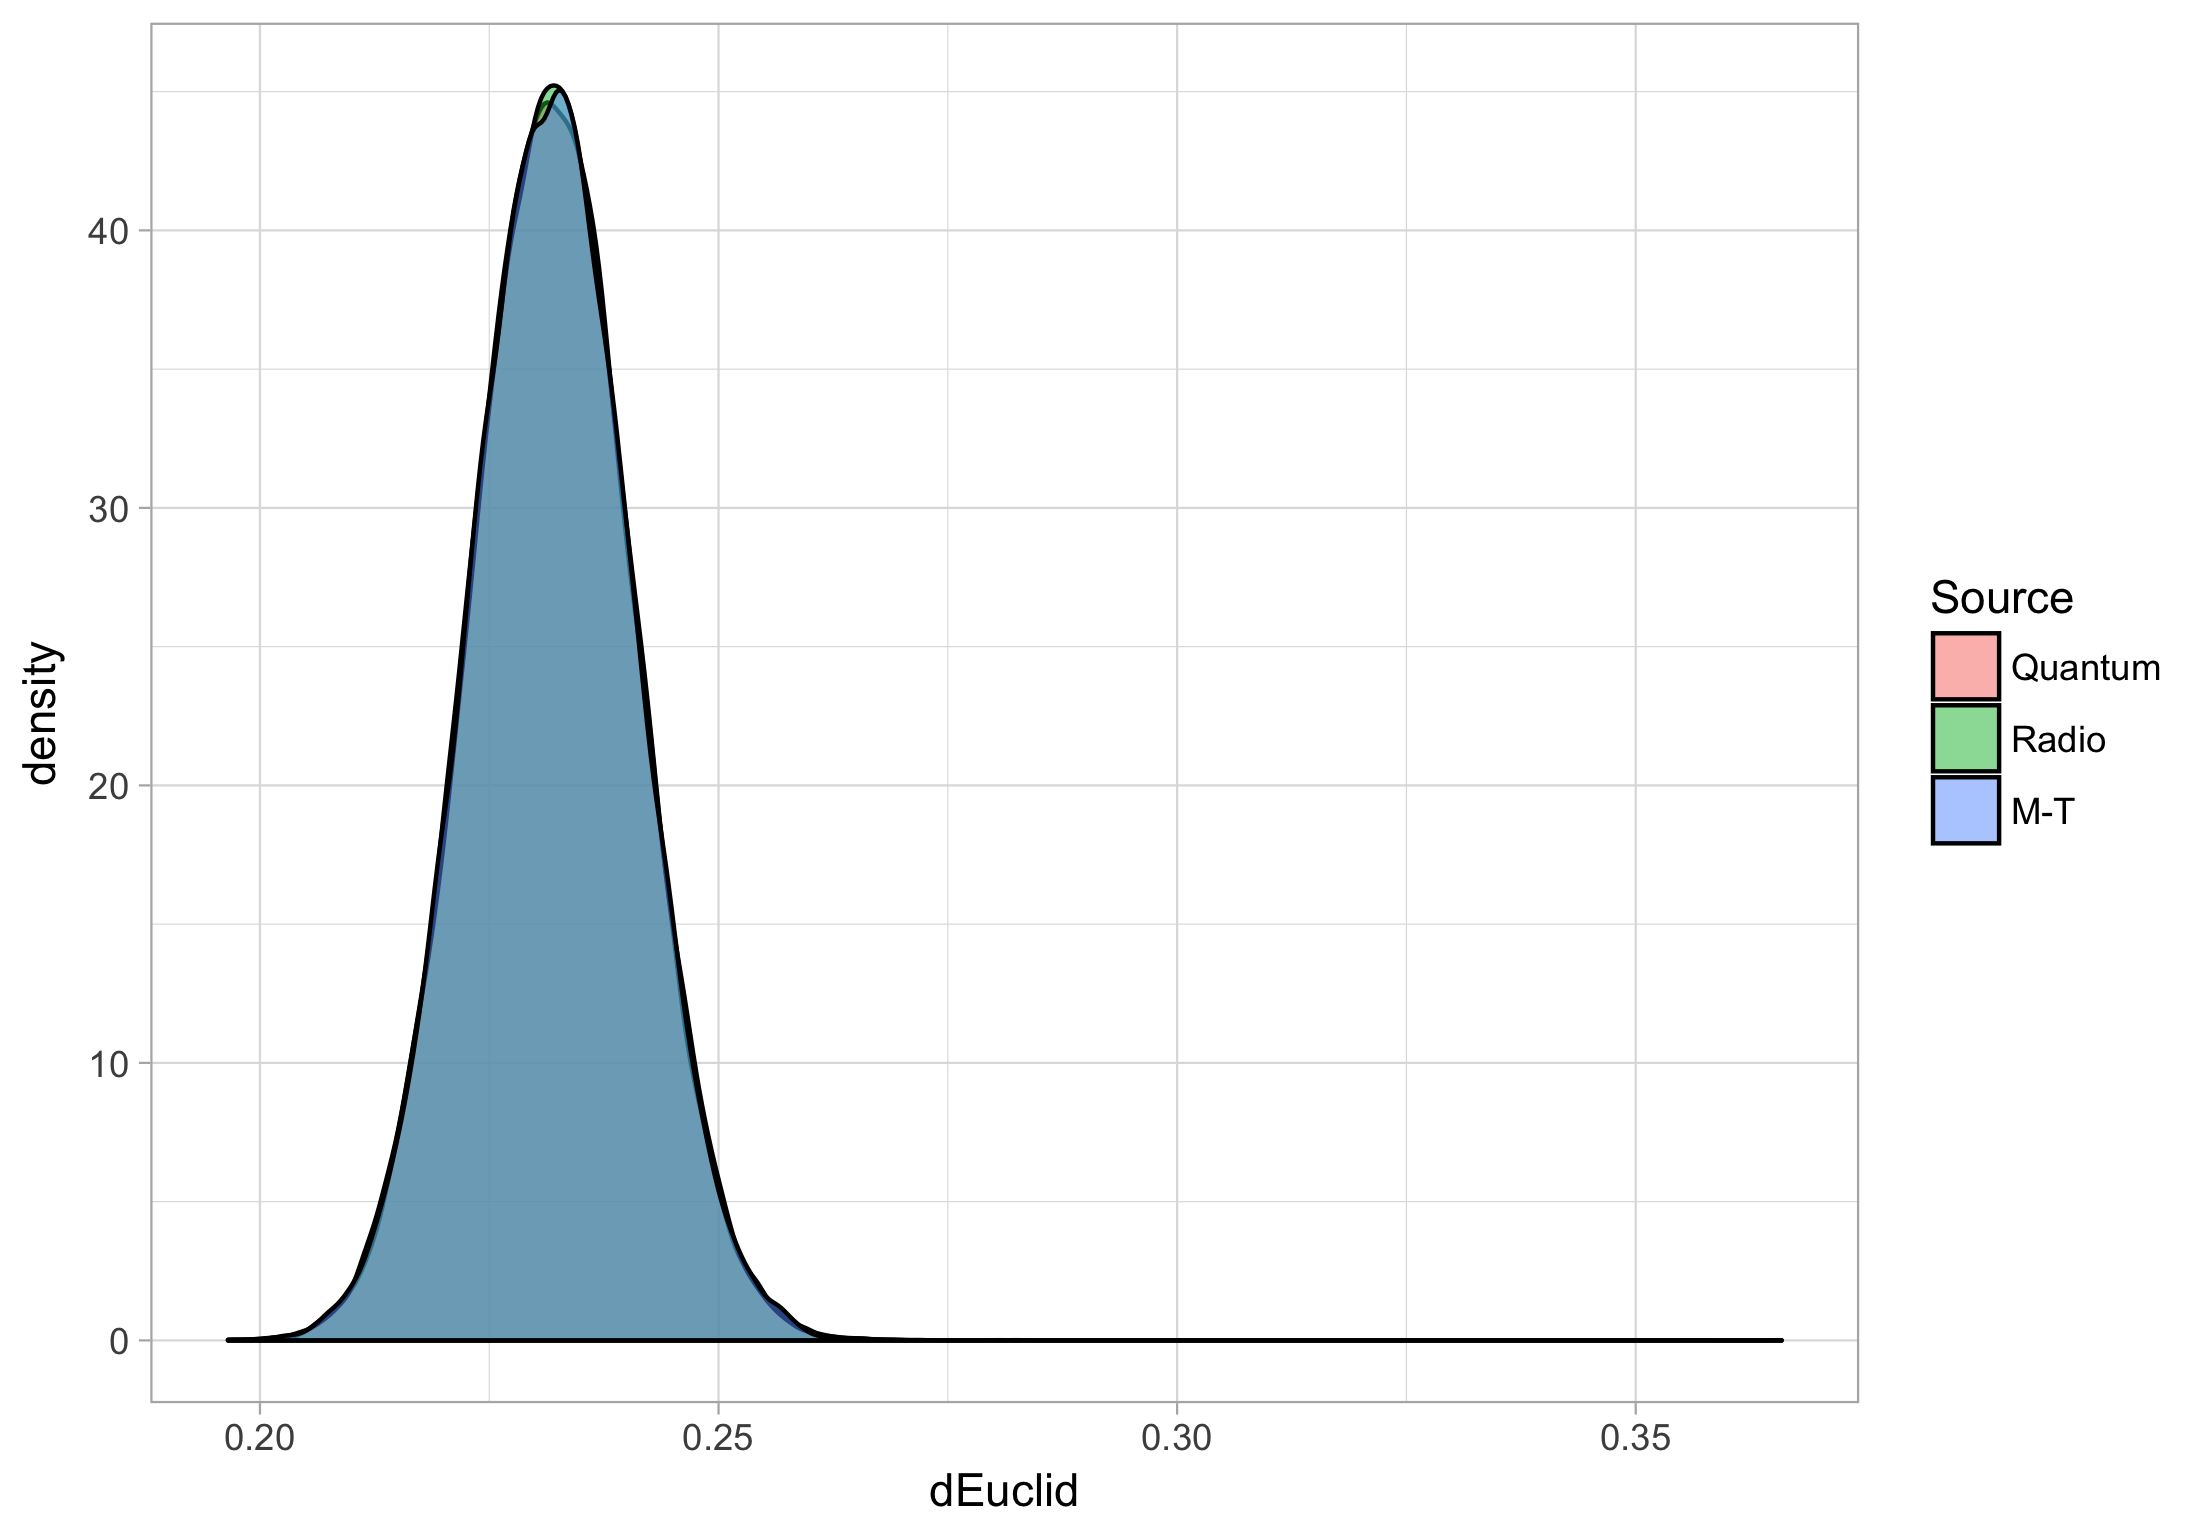
\includegraphics[width=.48\linewidth]{Hist_D6_1k_t50}}
		\caption{Histogramas suavizados de situações que sugerem que o gerador é um fator irrelevante para $N=1.000$}\label{fig:GeradorIrrelevante1k}
	\end{figure}
\end{block}
\end{frame}

\begin{frame}{Resultados}{Histogramas suavizados}
\begin{block}{}
\begin{figure} %D=6 %N 50000 t1 t 50
	\centering
	\subfigure[$D=6, \tau=1$]{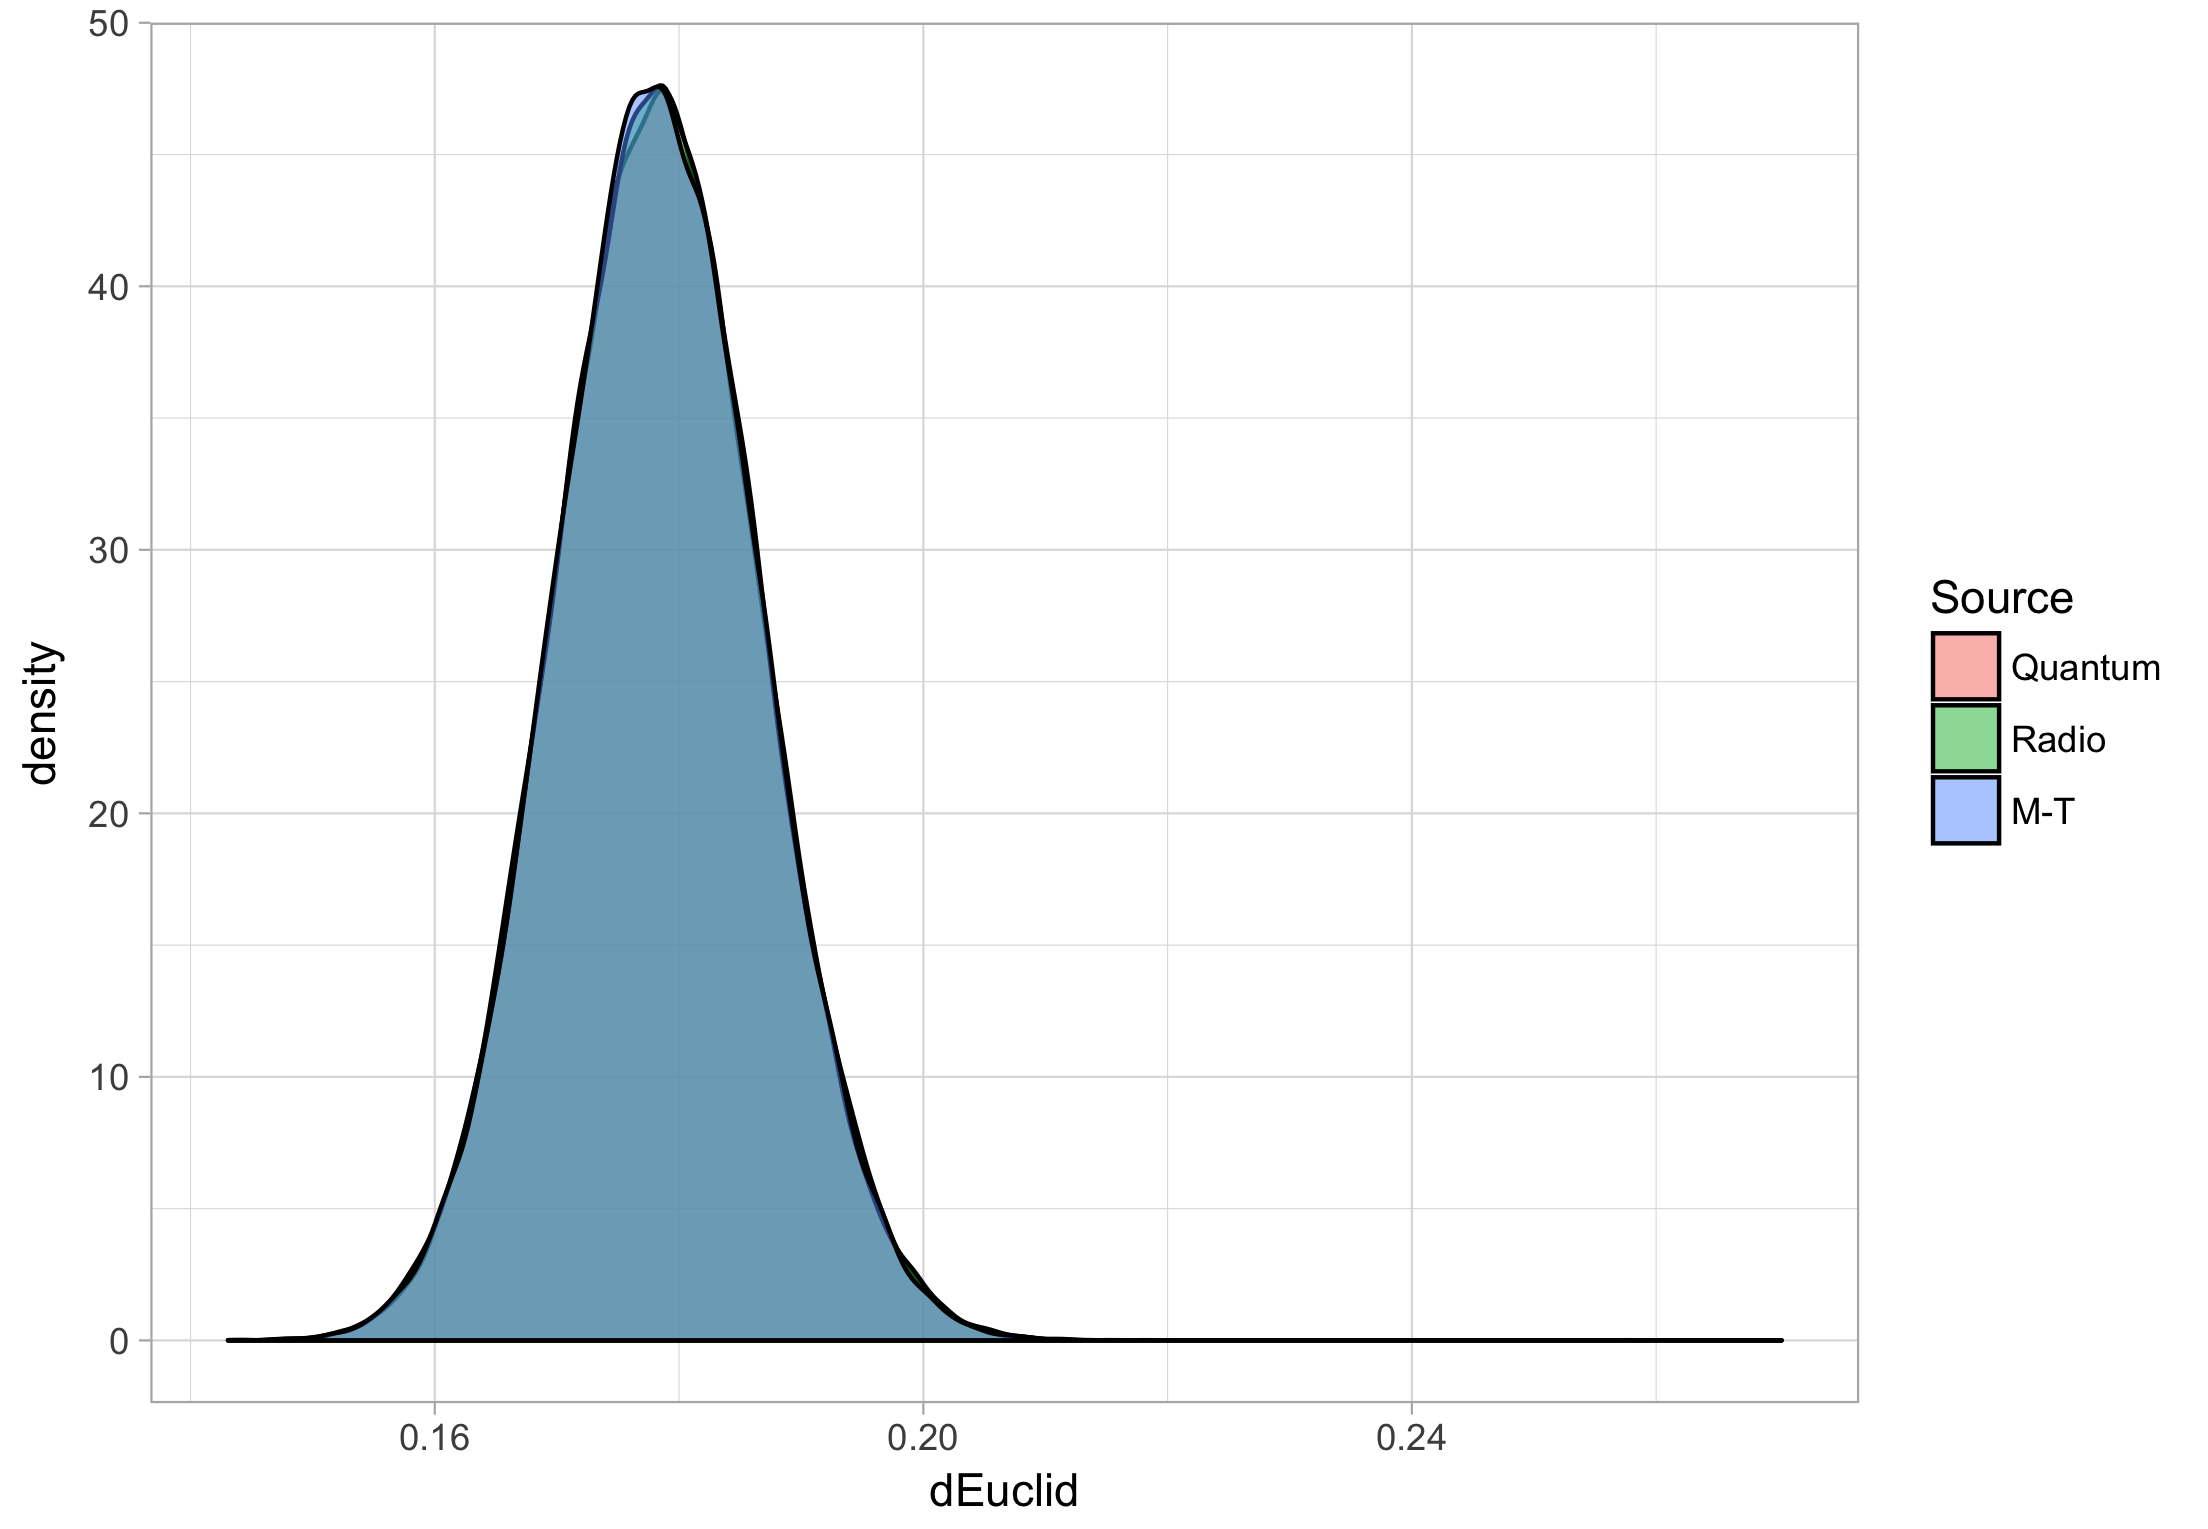
\includegraphics[width=.48\linewidth]{Hist_D6_50k_t1}}
	\subfigure[$D=6, \tau=50$]{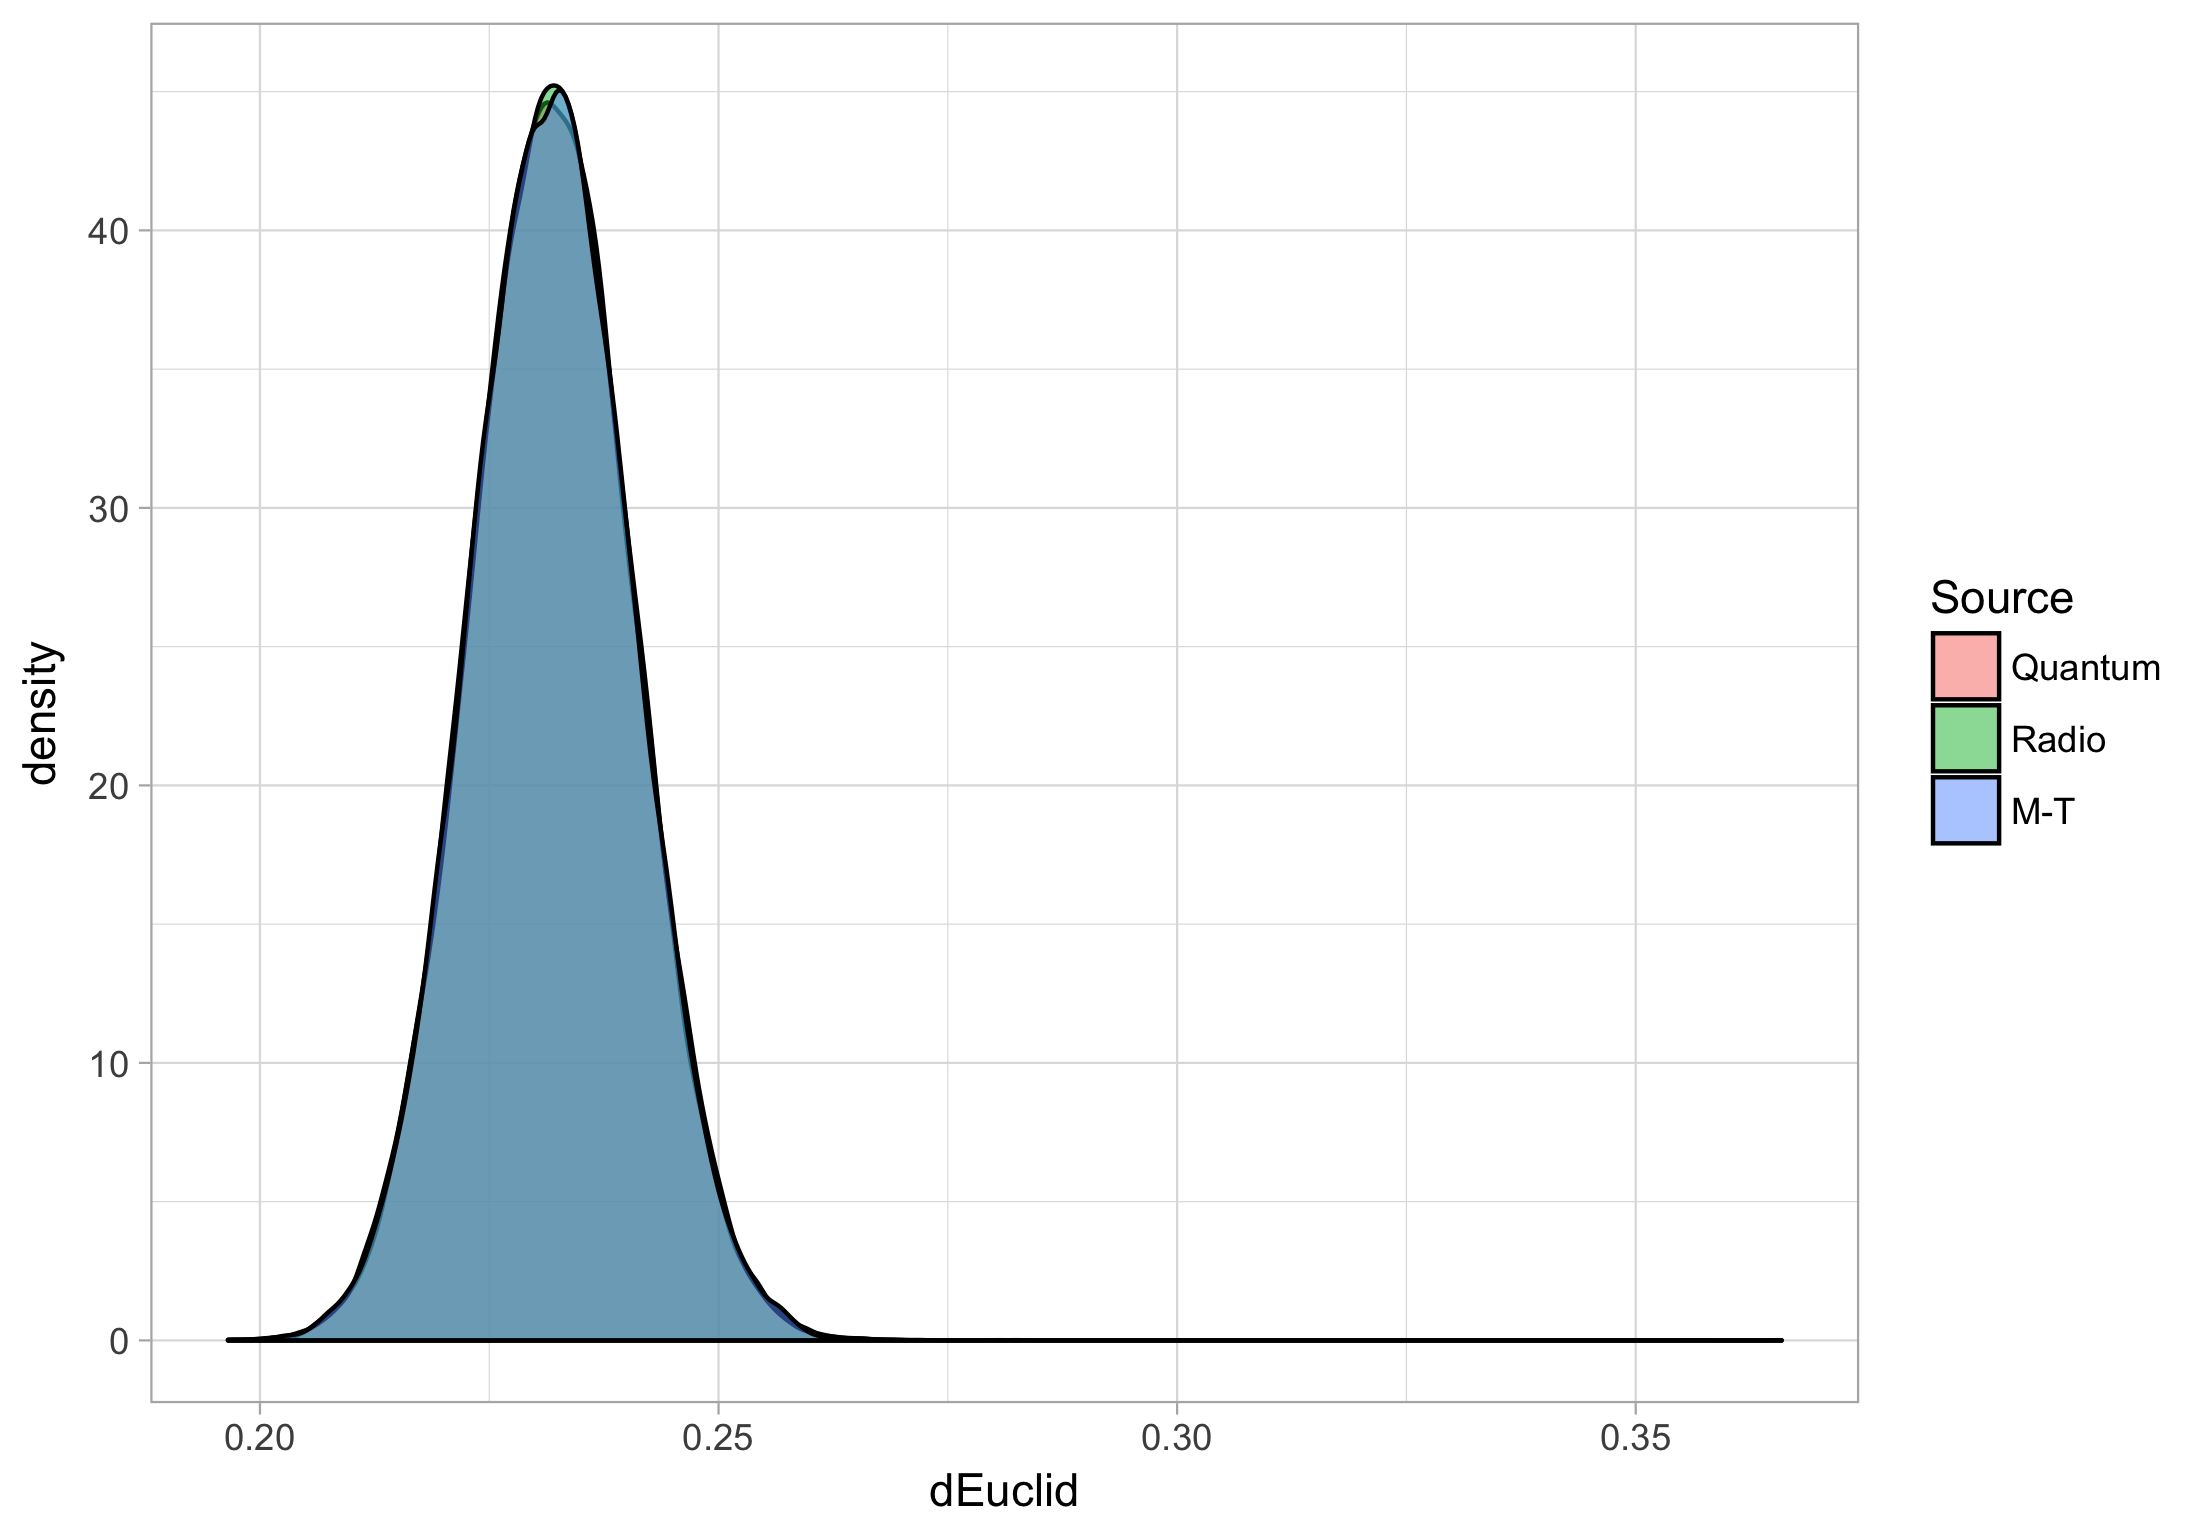
\includegraphics[width=.48\linewidth]{Hist_D6_50k_t50}}
	\caption{Histogramas suavizados de situações que sugerem que o gerador é um fator irrelevante também para $N=50.000$}\label{fig:GeradorIrrelevante50k}
\end{figure}
\end{block}
\end{frame}

\begin{frame}{Resultados}{Histogramas suavizados}
\begin{block}{}
	A figura a seguir mostra os histogramas suavizados das distâncias dos três geradores para palavras de tamanho $D=6$ e dois valores de \textit{lag} ($\tau=1$, $50$).
	
	\begin{figure} %D=6 %t 1 N 1000 N 50000 (três geradores) %t 50 N 1000 N 50000 (três geradores)
		\centering
		\subfigure[$D=6$, $\tau=1$]{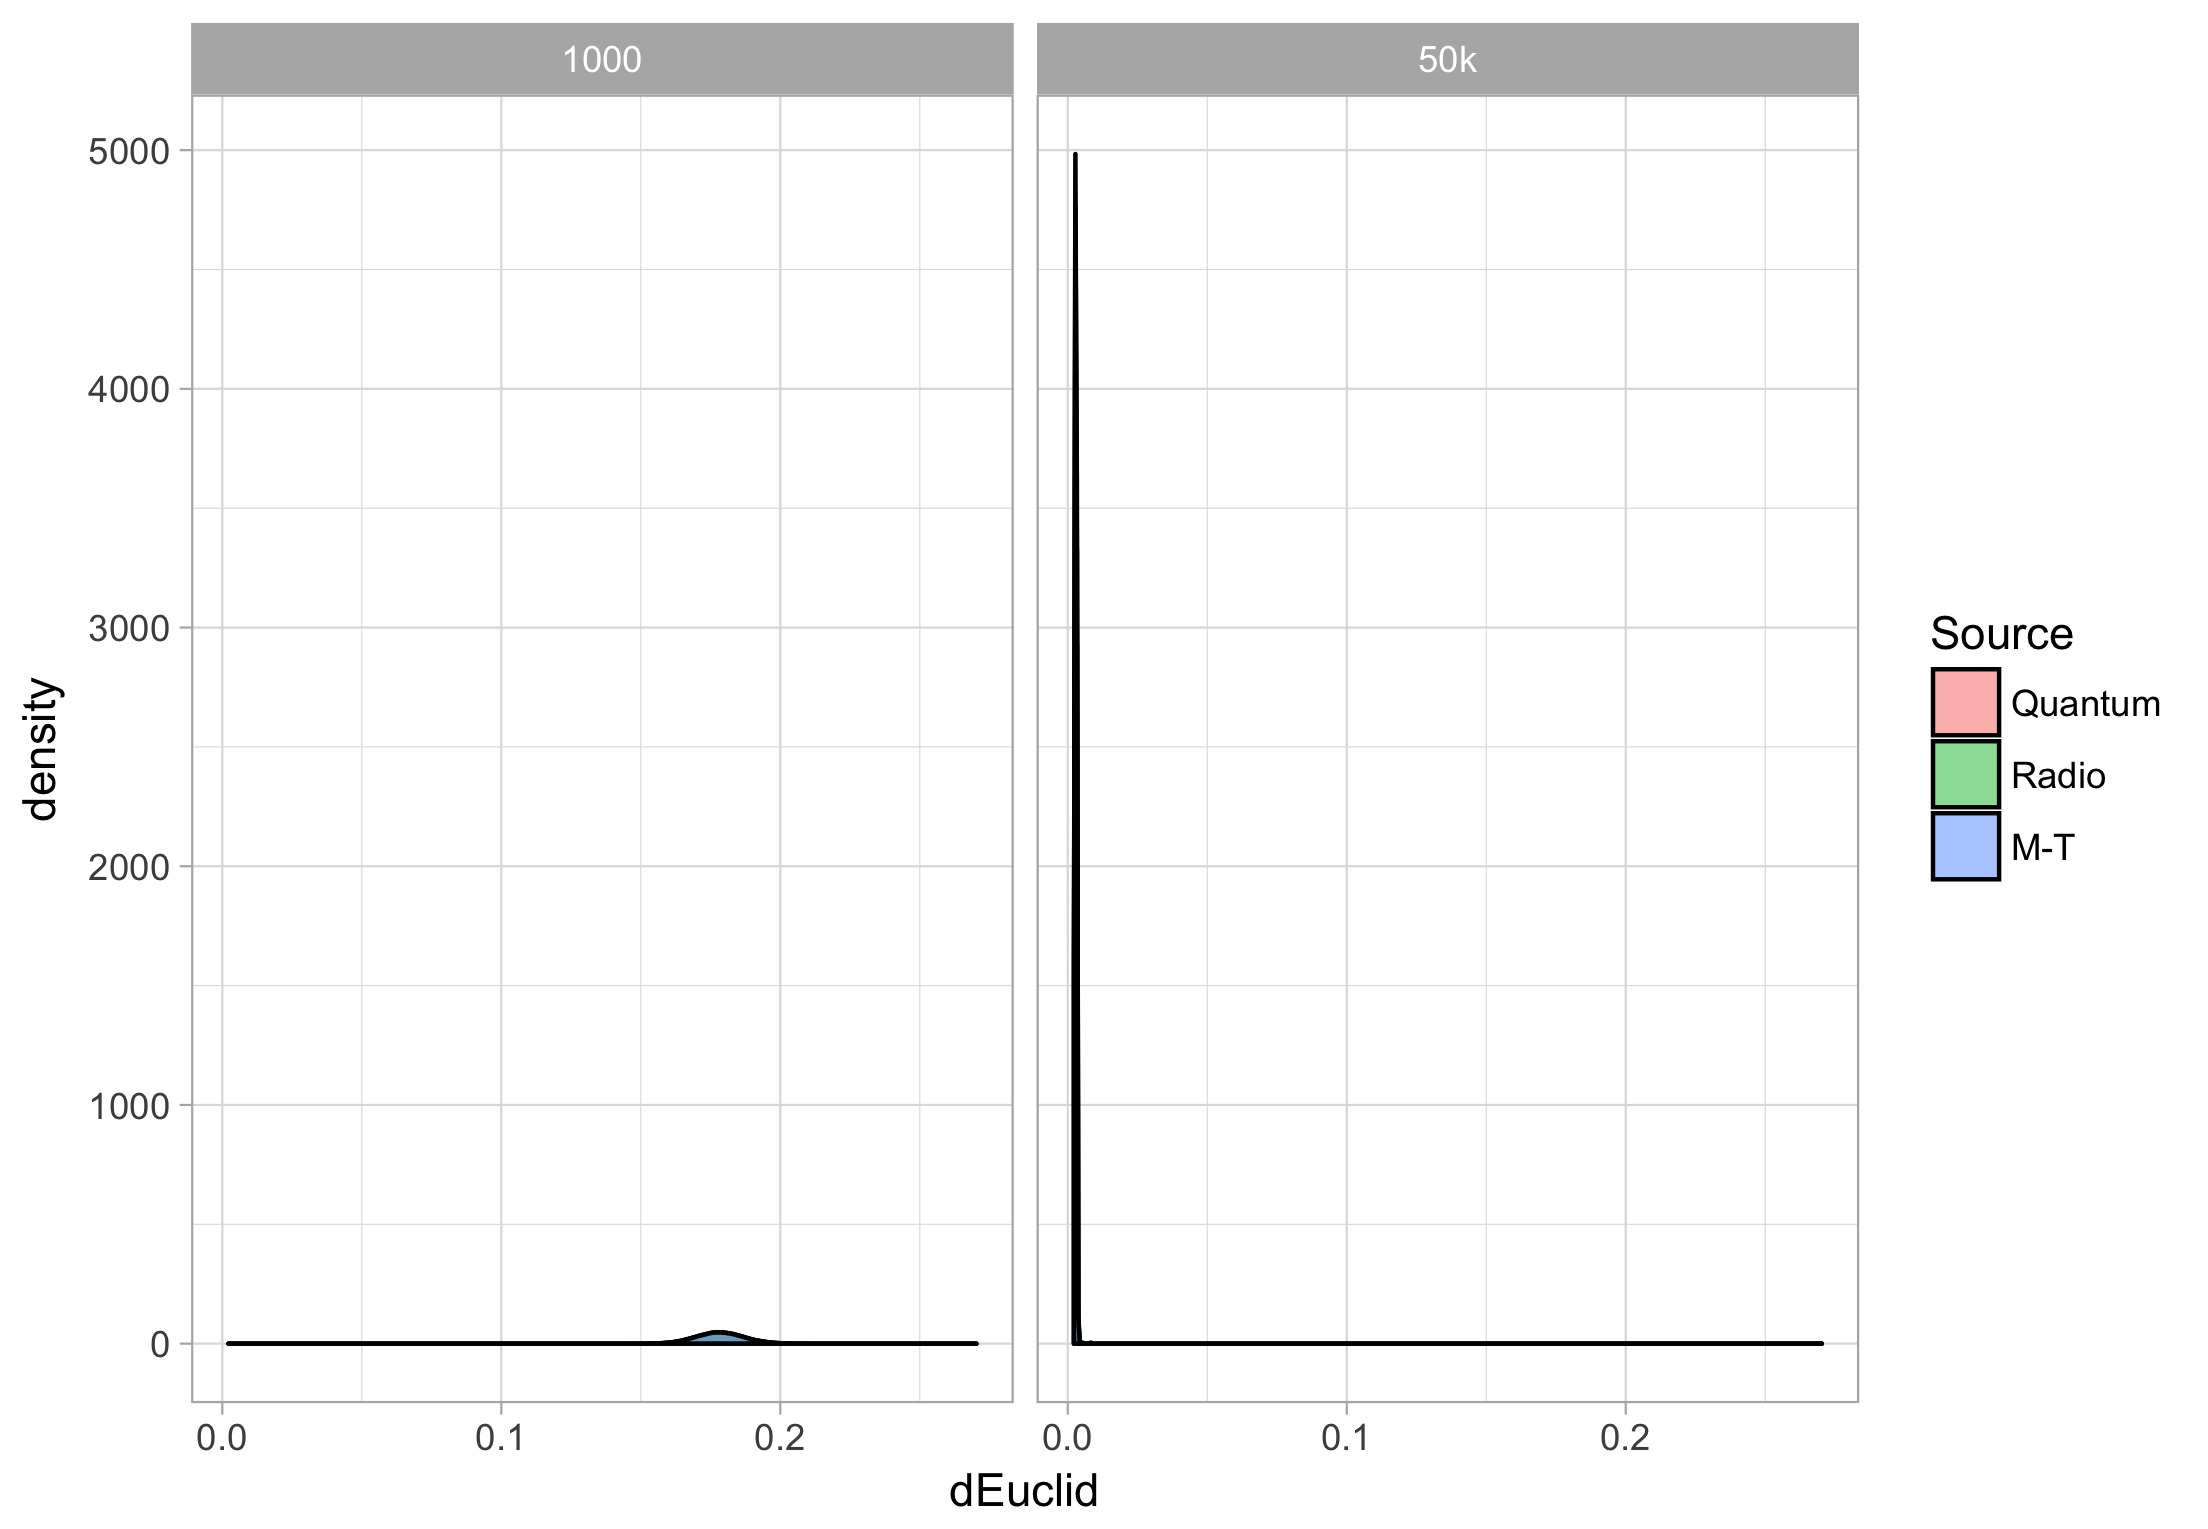
\includegraphics[width=.48\linewidth]{Hist_D6_t1}}
		\subfigure[$D=6$, $\tau=50$]{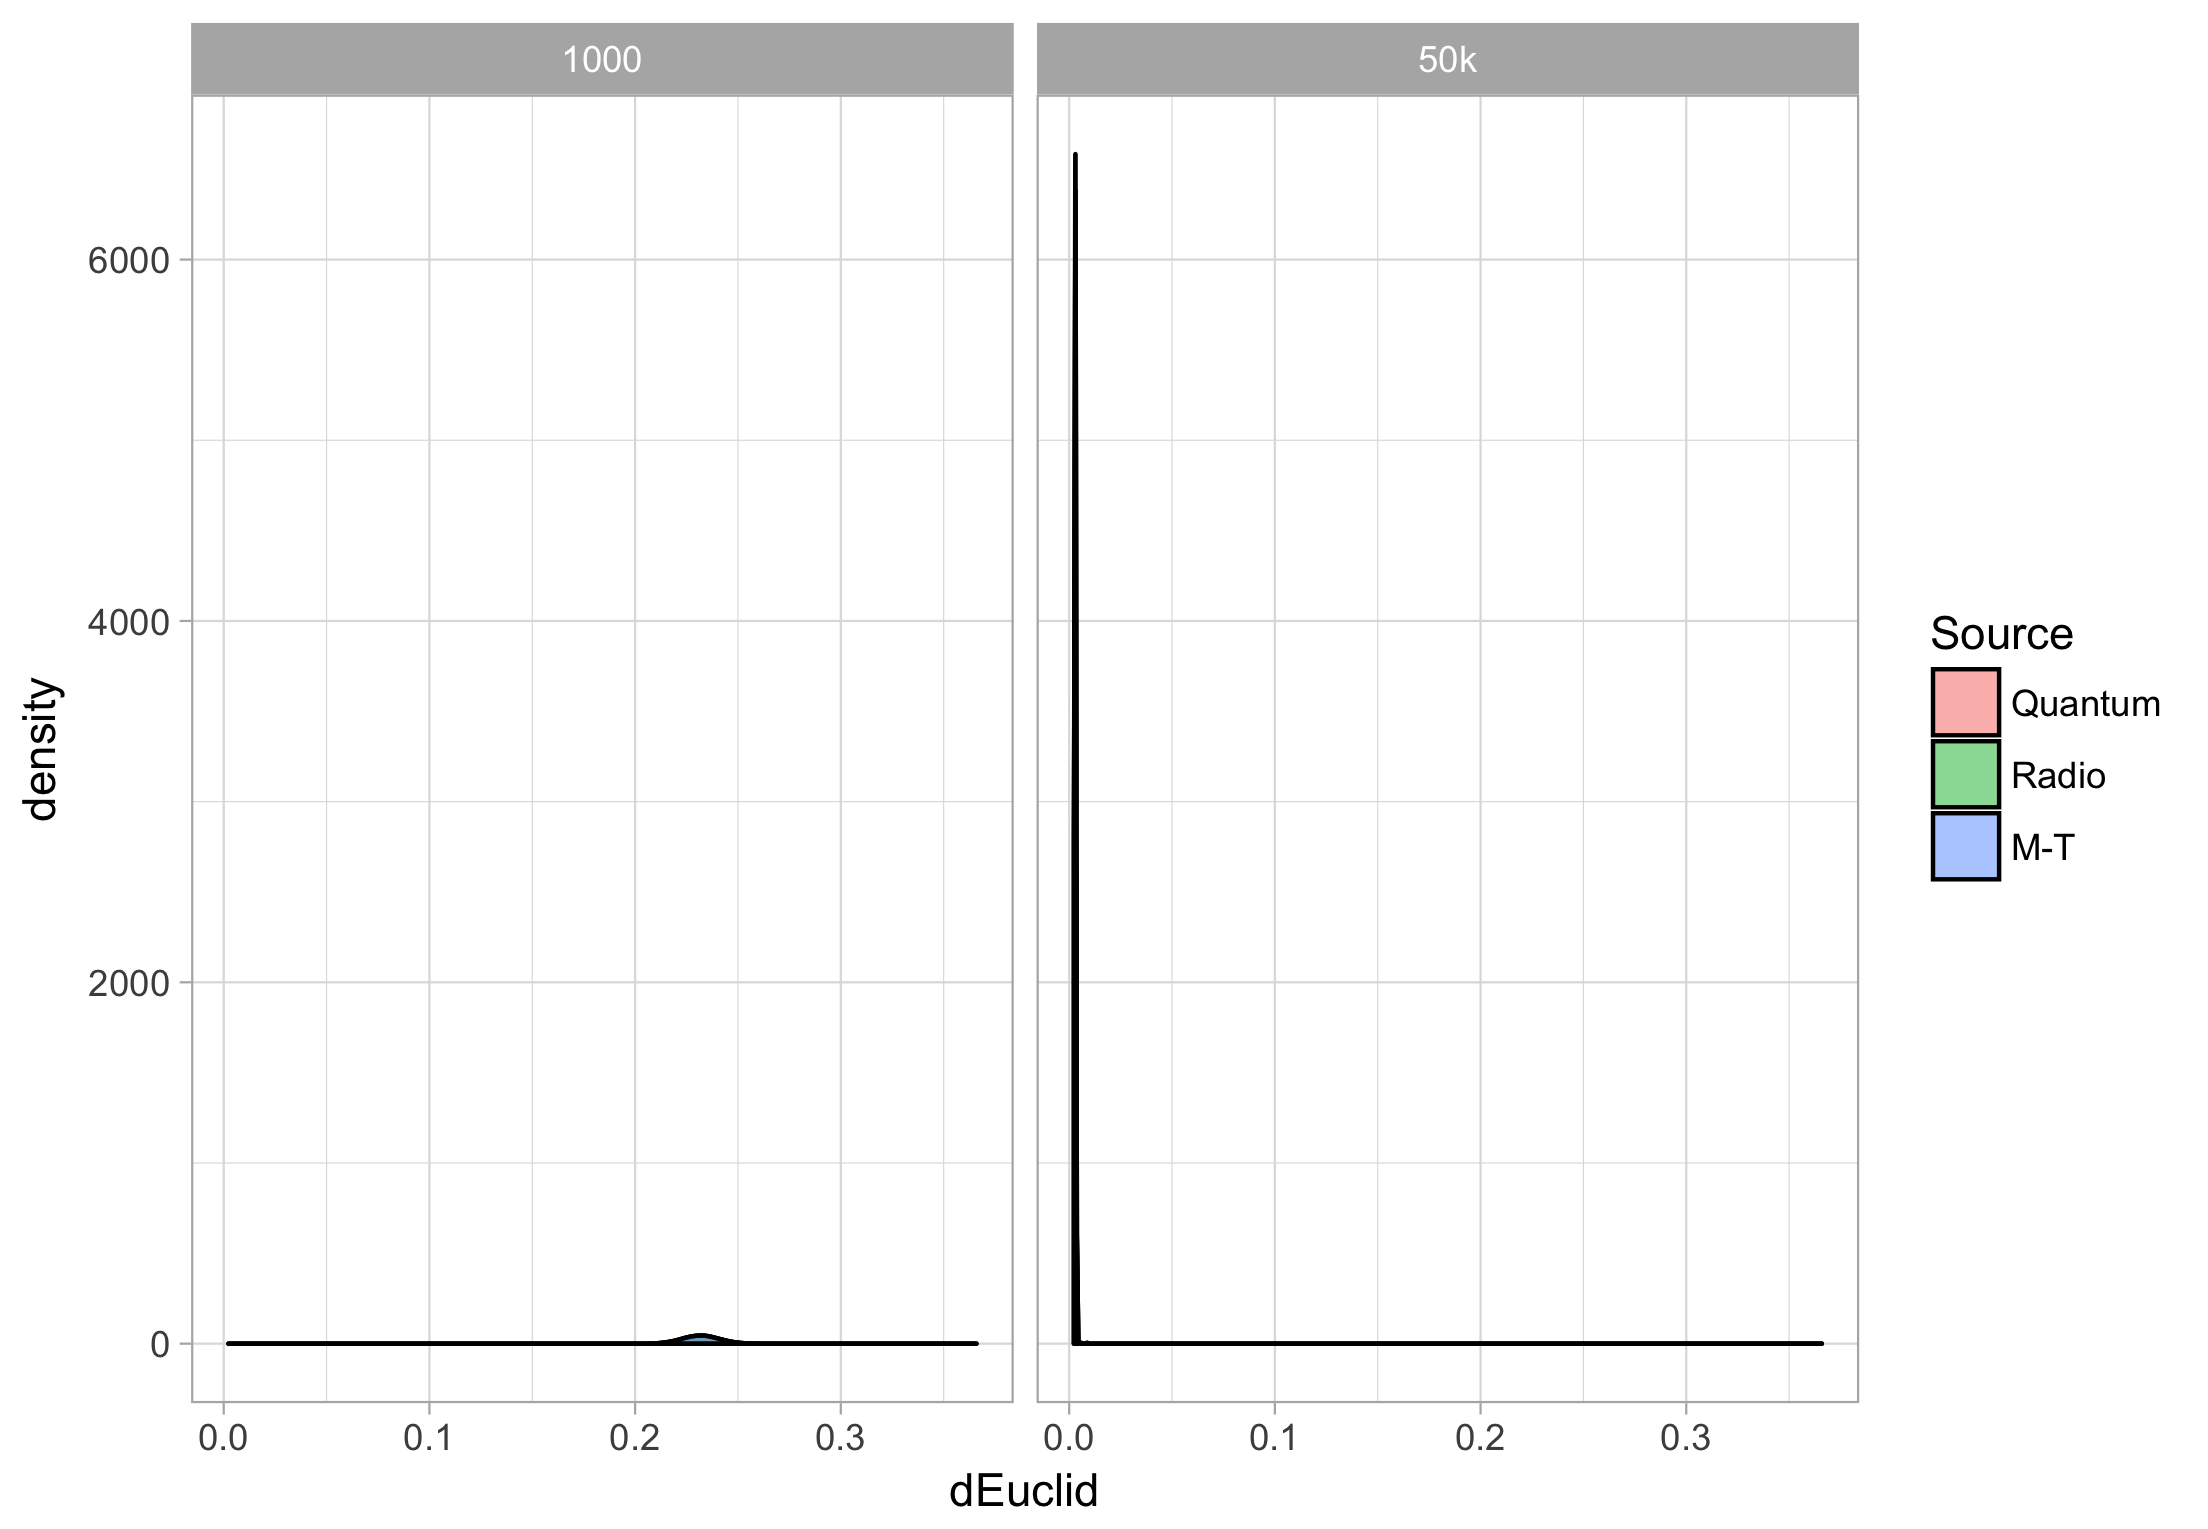
\includegraphics[width=.48\linewidth]{Hist_D6_t50}}
		\caption{Histogramas suavizados de situações que sugerem que o $N$ é um fator relevante}\label{fig:NRelevante}
	\end{figure}
\end{block}
\end{frame}

\begin{frame}{Resultados}{Histogramas suavizados}
\begin{block}{}
	A seguir mostramos os histogramas suavizados das distâncias dos três geradores para dois tamanhos de sequências ($N=1.000$, $50.000$) e dois valores de \textit{lag} ($\tau=1$, $50$).
	\begin{figure} %t 1 N 1000, D 3 D 4 D 5 D 6 %t 50 N 50000, D 3 D 4 D 5 D 6
		\centering
		\subfigure[$N=1.000$, $\tau=1$]{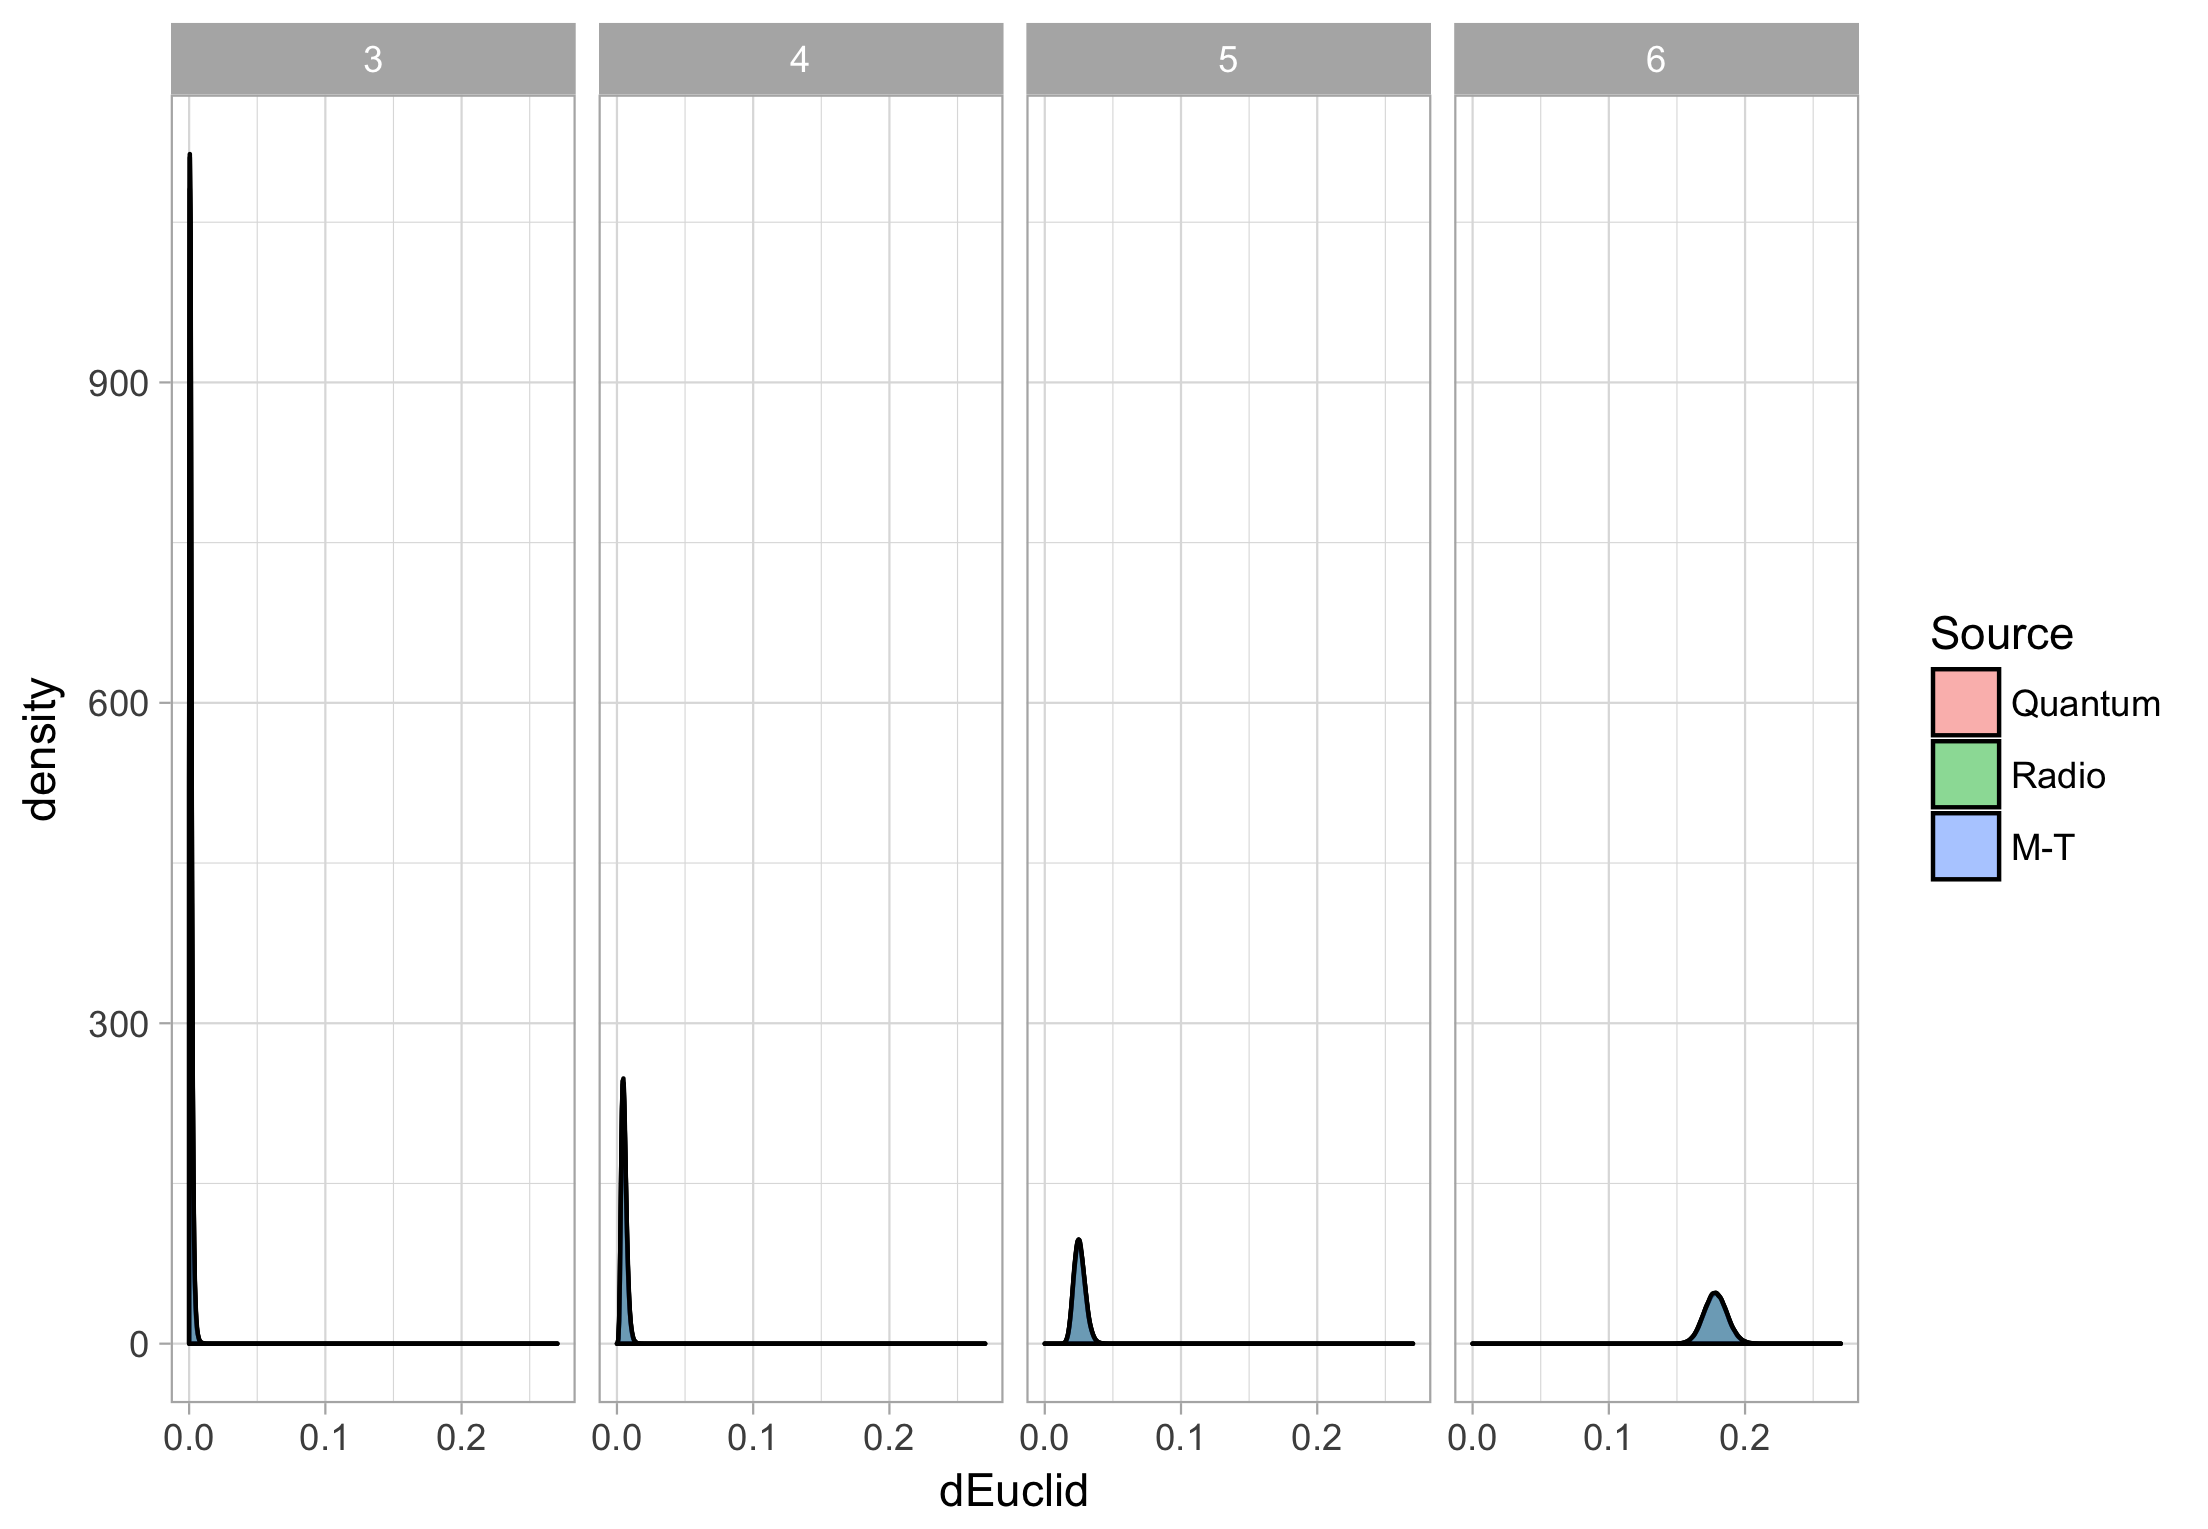
\includegraphics[width=.48\linewidth]{Hist_t1_1k}}
		\subfigure[$N=50.000$, $\tau=50$]{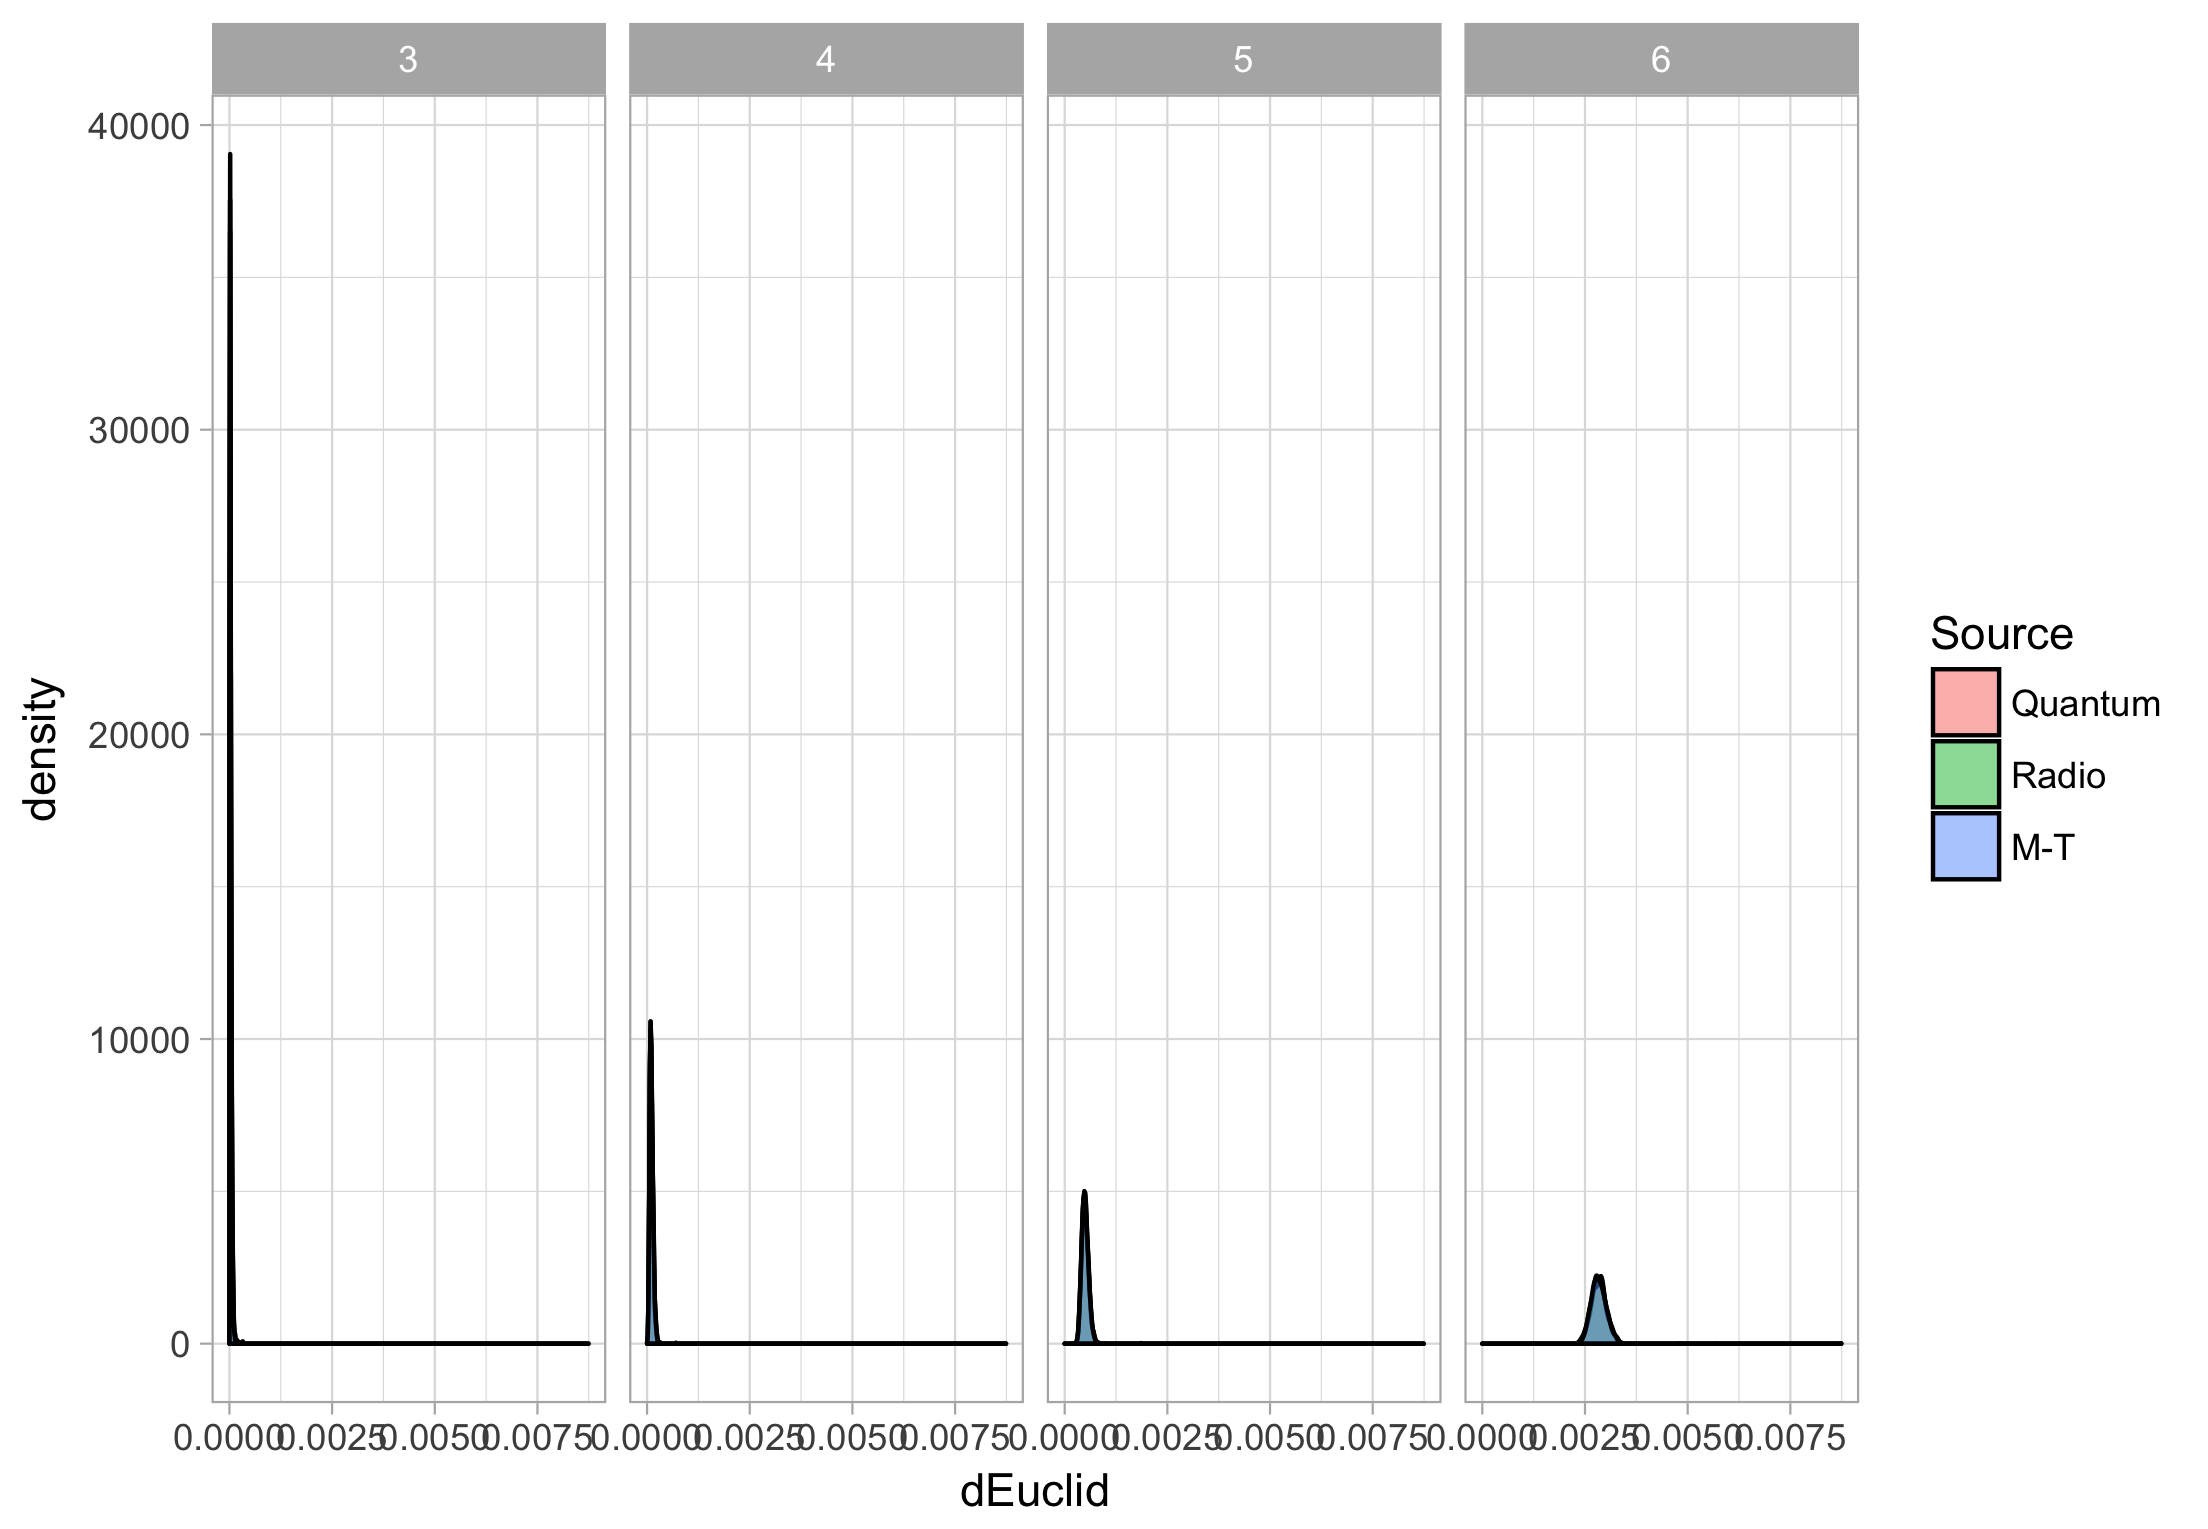
\includegraphics[width=.48\linewidth]{Hist_t50_50k}}
		\caption{Histogramas suavizados de situações que sugerem que o $D$ é um fator relevante}\label{fig:DRelevante}
	\end{figure}
\end{block}
\end{frame}

\begin{frame}{Resultados}{Histogramas suavizados}
\begin{block}{}
\begin{figure} %D 6 %N 1000, t 1 t 10 t 30 t 50 %N 50000, t 1 t 10 t 30 t 50
	A seguir mostramos os histogramas suavizados das distâncias dos três geradores para dois tamanhos de sequências ($N=1.000$, $50.000$) e $D=6$.
	\centering
	\subfigure[$N=1.000$, $D=6$]{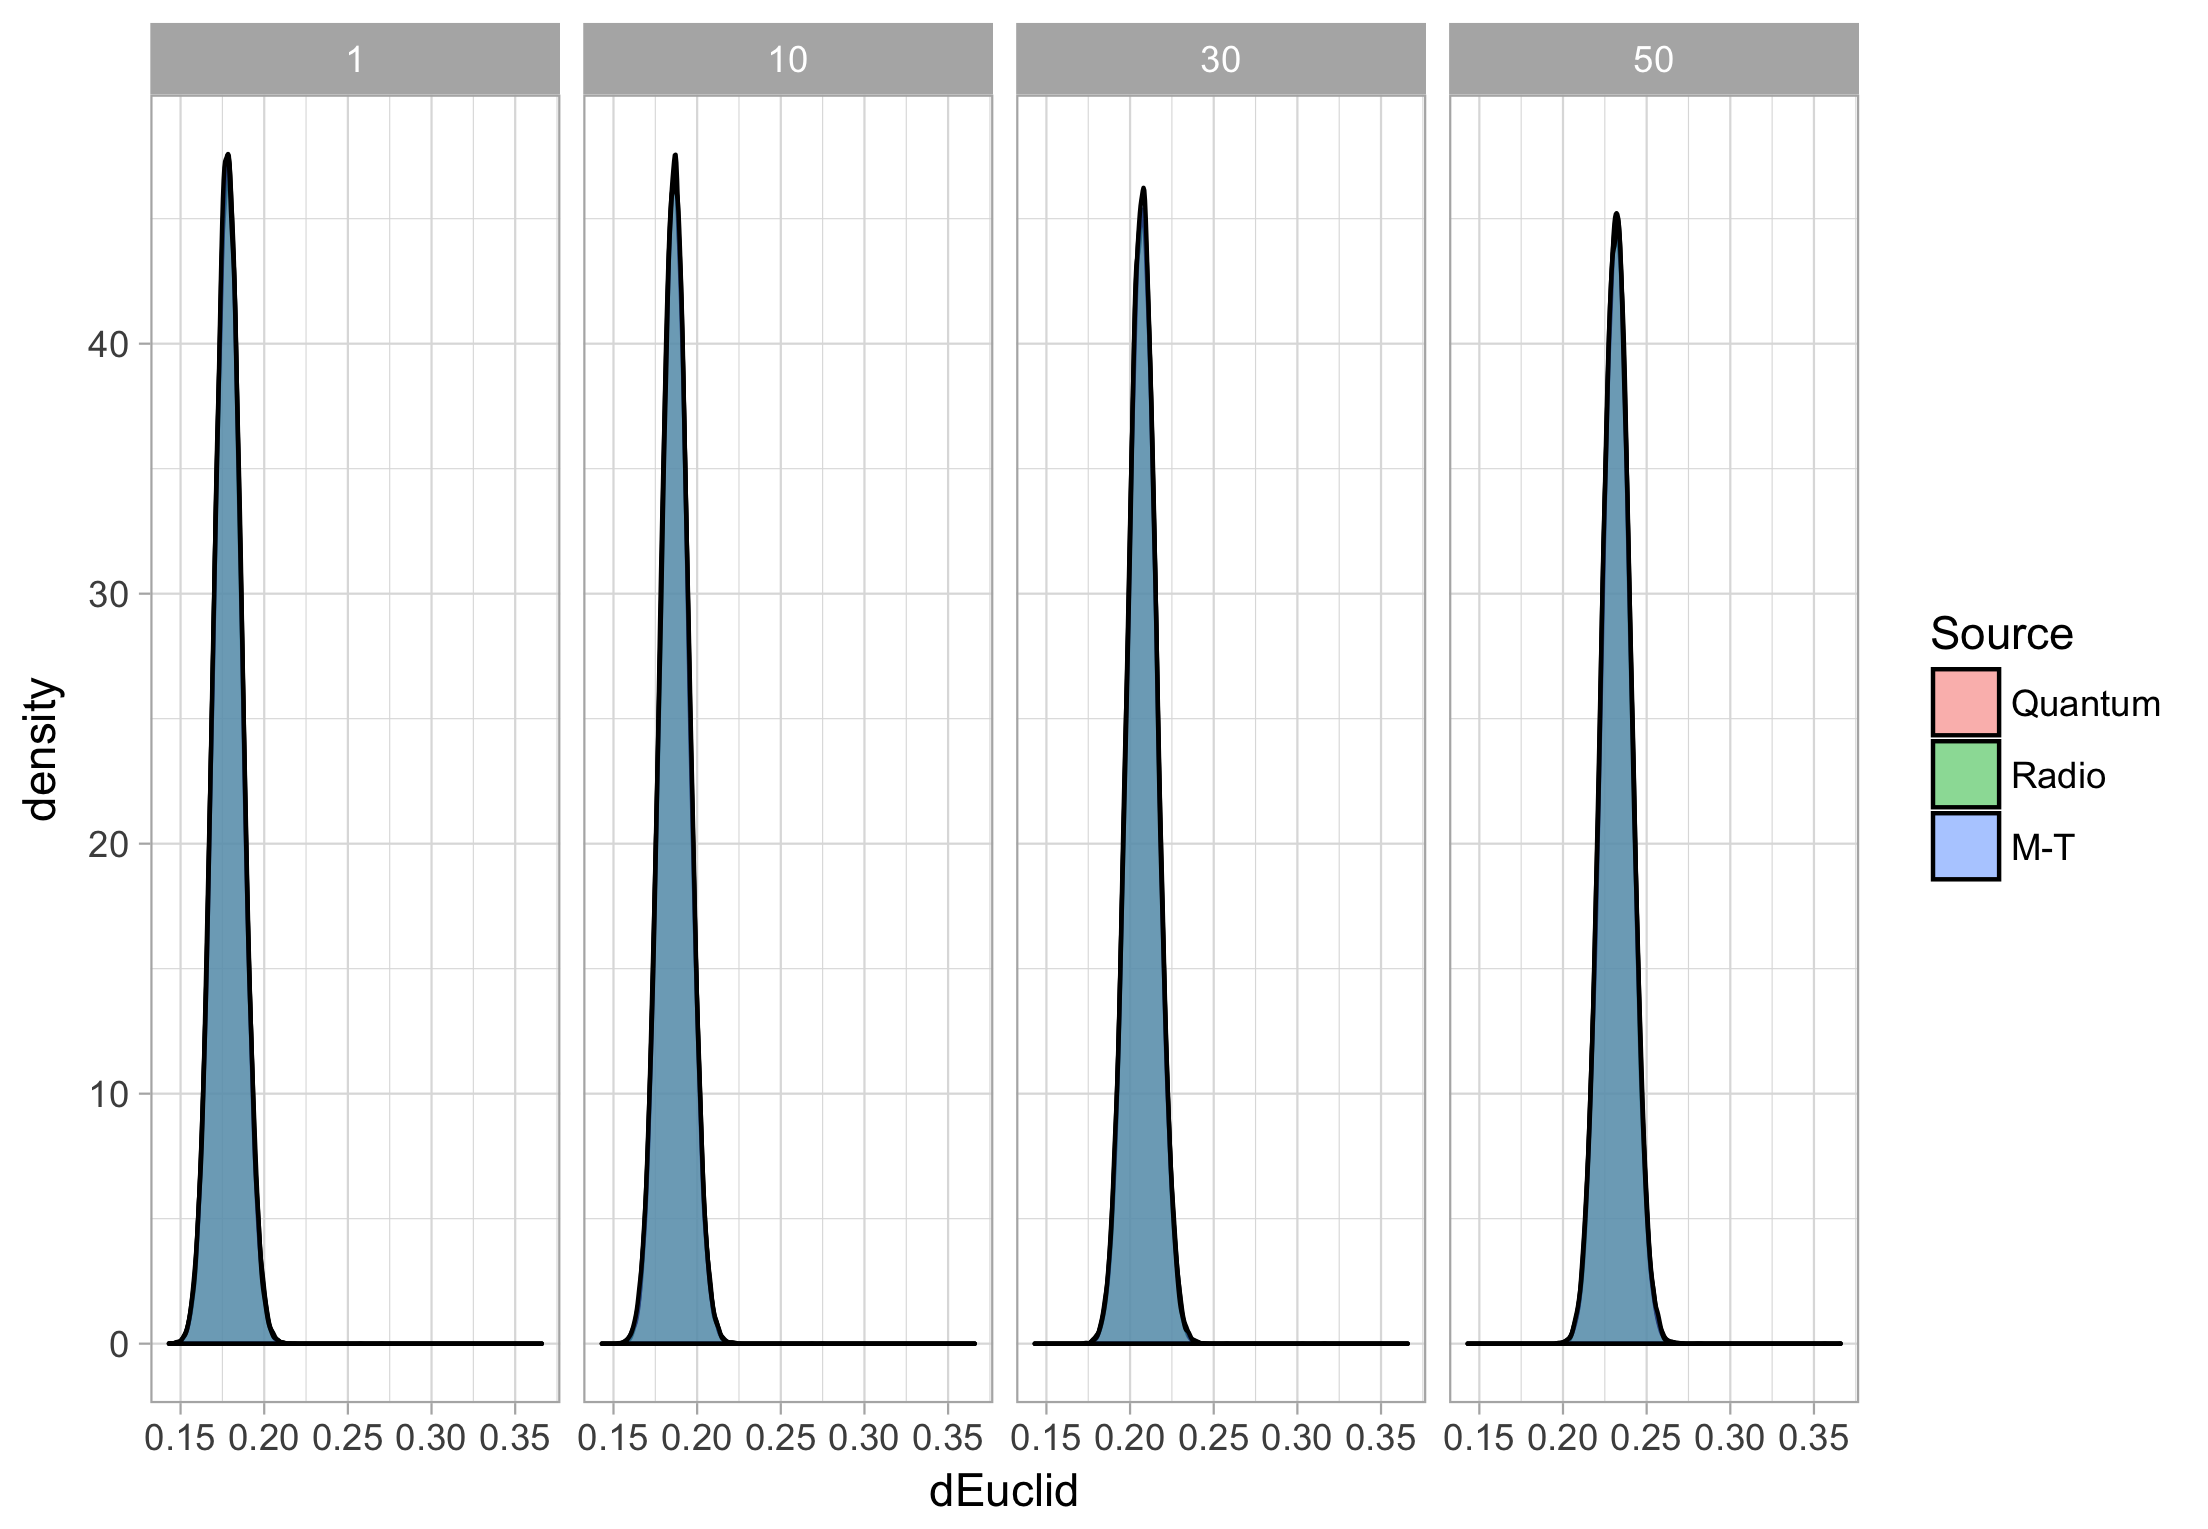
\includegraphics[width=.48\linewidth]{Hist_D6_1k}}
	\subfigure[$N=50.000$, $D=6$]{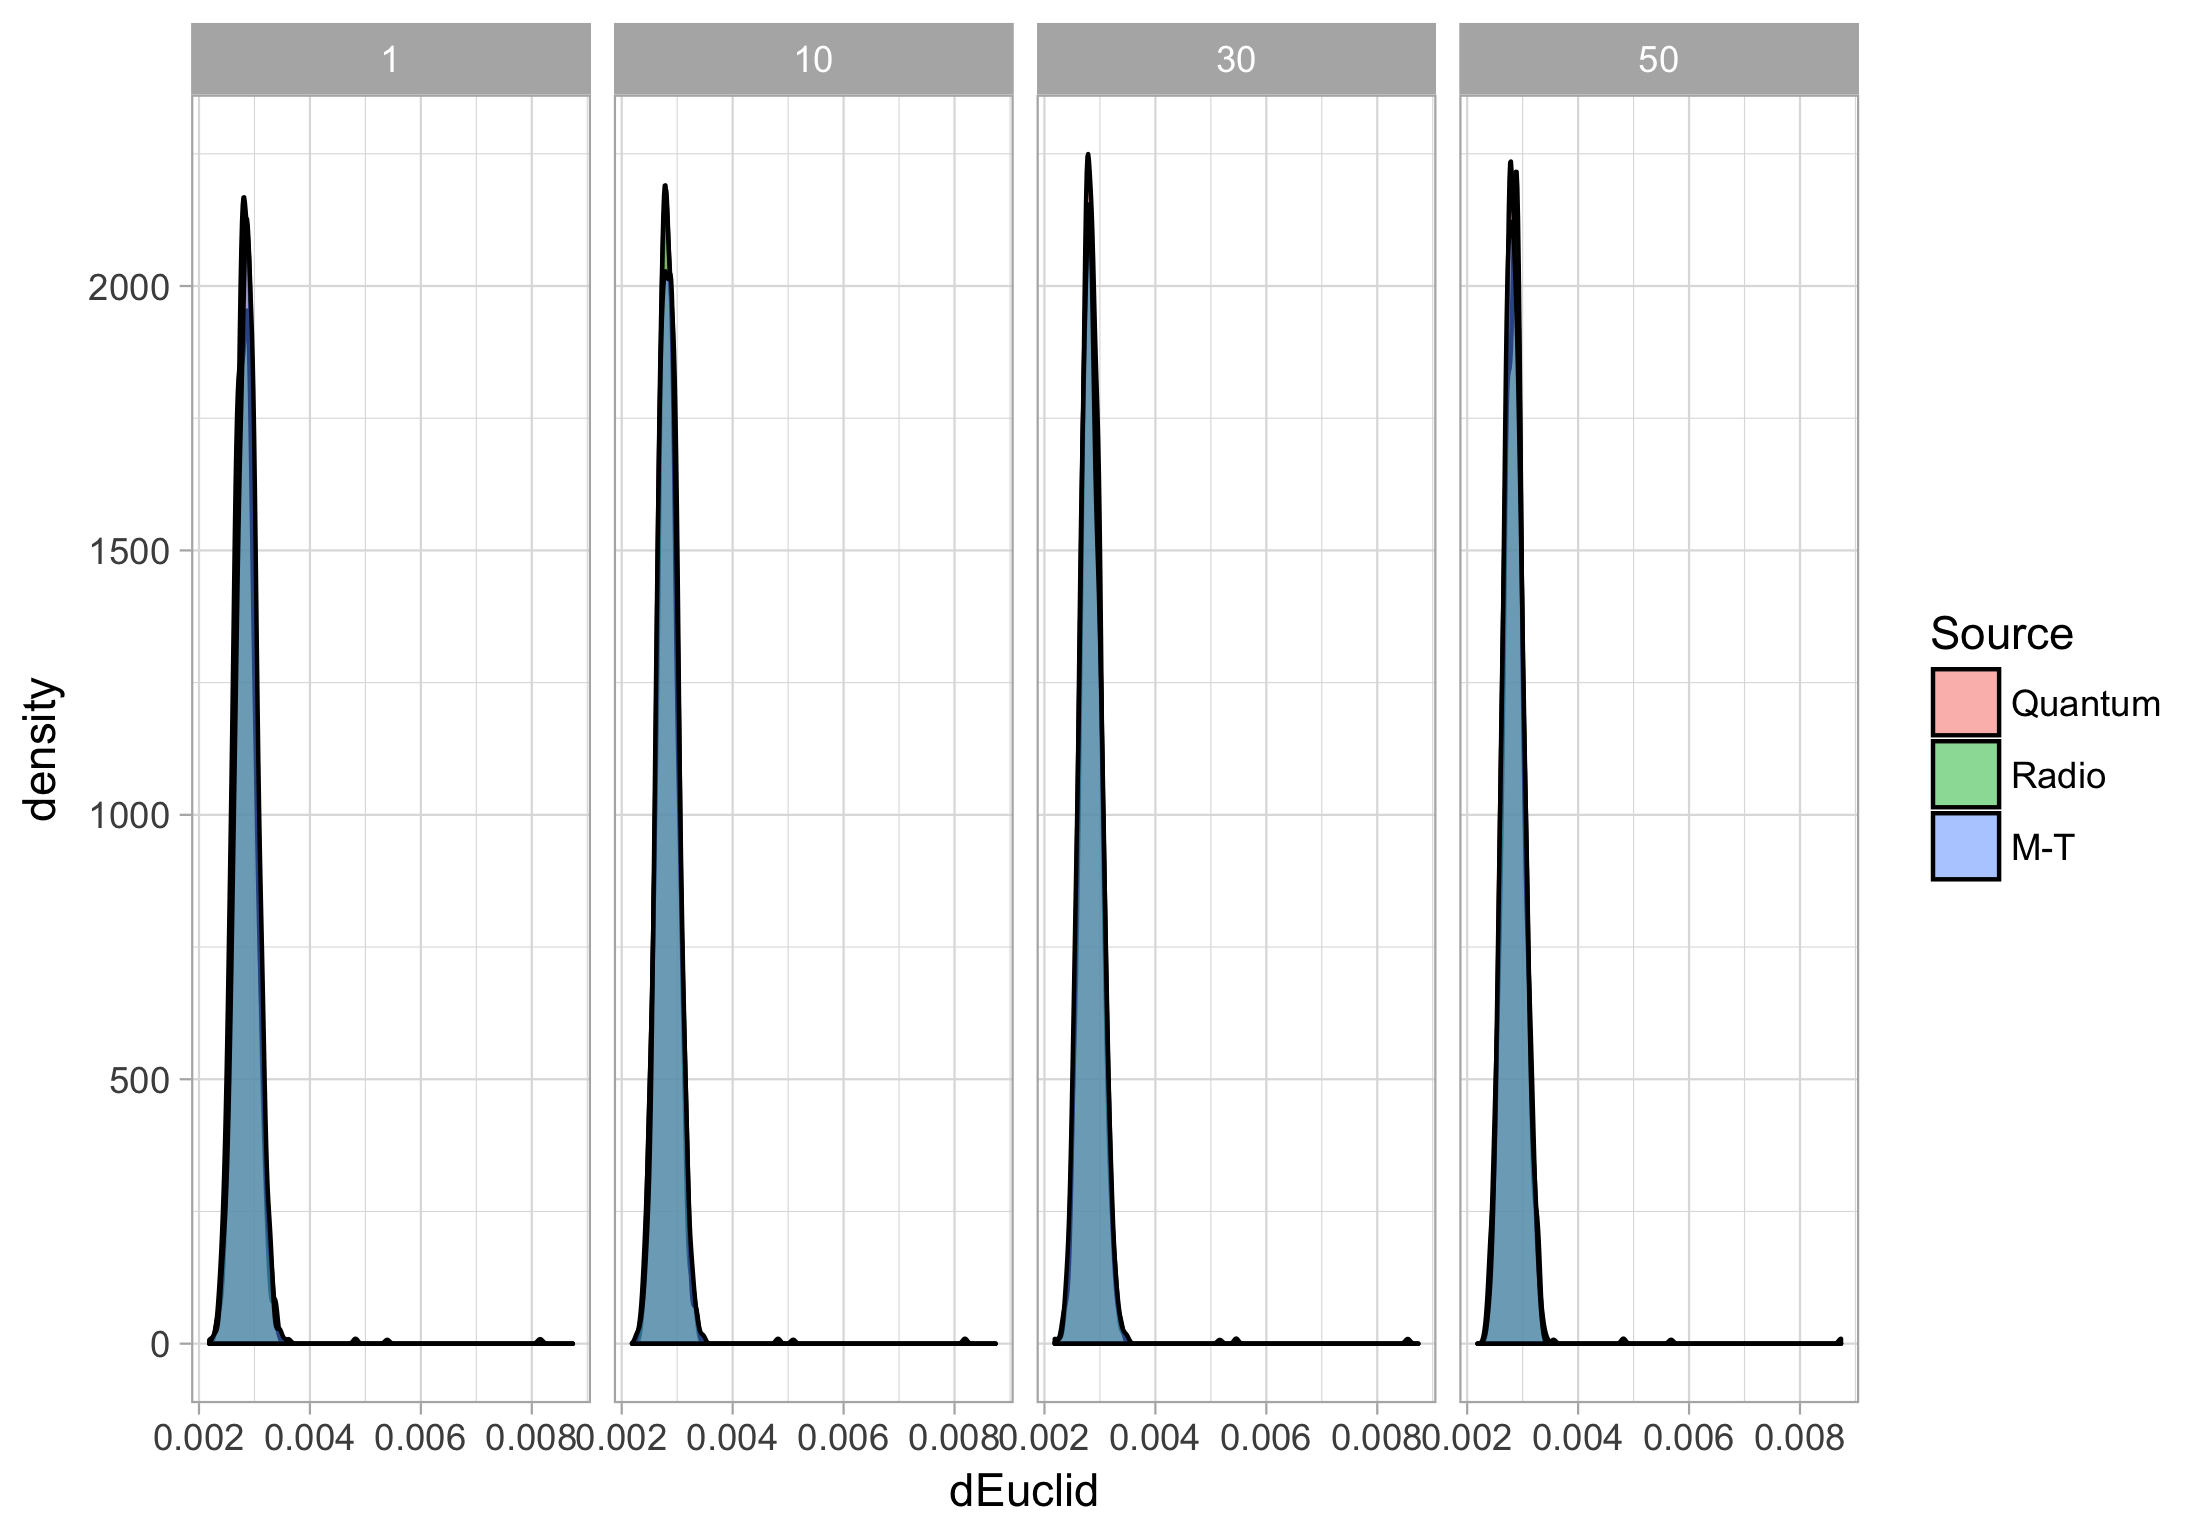
\includegraphics[width=.48\linewidth]{Hist_D6_50k}}
	\caption{Histogramas suavizados de situações que sugerem que o $\tau$ é um fator relevante}\label{fig:tRelevante}
\end{figure}	
\end{block}
\end{frame}

\begin{frame}{Resultados}{Teste de Kolmogorov-Smirnov}
\begin{block}{Teste de Kolmogorov-Smirnov aplicado a pares de sequências para $1.000$ observações}
\resizebox{\linewidth}{!}{% Resize table to fit within \linewidth horizontally	
		\centering
%		\caption{Teste de Kolmogorov-Smirnov aplicado a pares de sequências para $1.000$ observações.}\label{tab:KS_1000}
		\begin{tabular}{cccccc}
			\toprule
			Par  &    $D$ & $\tau=1$   &   $\tau=10$   &   $\tau=30$   &   $\tau=50$   \\ \midrule
			Quântica vs.\ Rádio		& $D=3$ & 0.18034676 & 0.08582490 & 0.58096350 & 0.32626542 \\
			& $D=4$ & 0.21708776 & 0.60690204 & 0.08116764 & 0.46372312  \\
			& $D=5$ & 0.32388371 & 0.53394280 & 0.46970138 & 0.02768674  \\
			& $D=6$ & 0.61501858 & 0.63403661 & 0.54795745 & 0.15353799  \\ \midrule
			Quântica vs. M-T & $D=3$ & 0.09400120 & 0.22995096 & 0.36766759 &  0.03706359 \\
			& $D=4$ & 0.25188769 & 0.35844686 & 0.16768952 &  0.18237754 \\
			& $D=5$ & 0.97552039 & 0.79878301 & 0.12852918 &  0.08764347 \\
			& $D=6$ & 0.47615384 & 0.42420007 & 0.55290011 &  0.79669144 \\ \midrule
			Rádio vs.\ M-T & $D=3$ & 0.008560614 & 0.496450214 & 0.982419336 & 0.390237891 \\
			& $D=4$ & 0.003804157 & 0.229503619 & 0.629158543 & 0.651783589 \\
			& $D=5$ & 0.254216237 & 0.179697451 & 0.824743440 & 0.071709252 \\
			& $D=6$ & 0.846441994 & 0.033726860 & 0.493286733 & 0.184856861 \\
			\bottomrule
		\end{tabular}}
	\end{block}
\end{frame}

\begin{frame}{Resultados}{Teste de Kolmogorov-Smirnov}
\begin{block}{Teste de Kolmogorov-Smirnov aplicado a pares de sequências para $50.000$ observações}
	\resizebox{\linewidth}{!}{% Resize table to fit within \linewidth horizontally	
		\begin{tabular}{cccccc}
			\toprule
		Par  & $D$ &   $\tau=1$   &   $\tau=10$   &   $\tau=30$   &   $\tau=50$   \\ \midrule
		Quântica vs.\ Rádio		& $D=3$ & 0.13862662 & 0.93677447 & 0.07714702 &  0.46405291 \\
		& $D=4$ & 0.68079537 & 0.90035466 & 0.60801914 &  0.77908261 \\
		& $D=5$ & 0.14371256 & 0.76662067 & 0.64456996 &  0.91315843 \\
		& $D=6$ & 0.02268670 & 0.49307044 & 0.53135926 &  0.30074267 \\ \midrule
		Quântica vs.\ M-T & $D=3$ & 6.074571e-10 & 1.388898e-01 & 2.682058e-01 & 4.822849e-01 \\
		& $D=4$ & 6.592620e-09 & 2.987721e-02 & 8.438134e-01 & 7.923220e-01 \\
		& $D=5$ & 9.424114e-08 & 3.289299e-02 & 7.681676e-01 & 8.405168e-01 \\
		& $D=6$ & 9.058821e-04 & 7.075225e-01 & 2.982731e-01 & 3.614763e-01 \\ \midrule
		Rádio vs.\ M-T		& $D=3$ & 1.226271e-09 & 1.609665e-01 & 1.465970e-01 & 1.914937e-01 \\
		& $D=4$ & 2.190462e-10 & 1.277762e-02 & 2.069821e-01 & 9.963221e-01 \\
		& $D=5$ & 1.438372e-11 & 1.267622e-02 & 4.364935e-01 & 9.999998e-01 \\
		& $D=6$ & 3.749001e-06 & 2.263466e-01 & 7.419248e-01 & 4.014641e-01 \\
		\bottomrule
	\end{tabular}}
\end{block}
\end{frame}

\begin{frame}{Resultados}{Teste de Kolmogorov-Smirnov}
\begin{block}{Teste de Kolmogorov-Smirnov aplicado a pares de sequências para $50.000$ observações}
	\resizebox{\linewidth}{!}{% Resize table to fit within \linewidth horizontally	
		\begin{tabular}{cccccc}
			\toprule
			Par  & $D$ &   $\tau=1$   &   $\tau=10$   &   $\tau=30$   &   $\tau=50$   \\ \midrule
			Quântica vs.\ Rádio		& $D=3$ & 0.13862662 & 0.93677447 & 0.07714702 &  0.46405291 \\
			& $D=4$ & 0.68079537 & 0.90035466 & 0.60801914 &  0.77908261 \\
			& $D=5$ & 0.14371256 & 0.76662067 & 0.64456996 &  0.91315843 \\
			& $D=6$ & 0.02268670 & 0.49307044 & 0.53135926 &  0.30074267 \\ \midrule
			Quântica vs.\ M-T & $D=3$ & \textbf{6.074571e-10} & 1.388898e-01 & 2.682058e-01 & 4.822849e-01 \\
			& $D=4$ & \textbf{6.592620e-09} & 2.987721e-02 & 8.438134e-01 & 7.923220e-01 \\
			& $D=5$ & \textbf{9.424114e-08} & 3.289299e-02 & 7.681676e-01 & 8.405168e-01 \\
			& $D=6$ & \textbf{9.058821e-04} & 7.075225e-01 & 2.982731e-01 & 3.614763e-01 \\ \midrule
			Rádio vs.\ M-T		& $D=3$ & \textbf{1.226271e-09} & 1.609665e-01 & 1.465970e-01 & 1.914937e-01 \\
			& $D=4$ & \textbf{2.190462e-10} & 1.277762e-02 & 2.069821e-01 & 9.963221e-01 \\
			& $D=5$ & \textbf{1.438372e-11} & 1.267622e-02 & 4.364935e-01 & 9.999998e-01 \\
			& $D=6$ & \textbf{3.749001e-06} & 2.263466e-01 & 7.419248e-01 & 4.014641e-01 \\
			\bottomrule
	\end{tabular}}
\end{block}
\end{frame}


\begin{frame}{Resultados}{}
\begin{block}{}
	Os $p$-valores observados na Tabela de teste de Kolmogorov-Smirnov aplicado a pares de sequências para $50.000$ observações nos levam a concluir que não é possível desconsiderar a fonte de dados como um fator relevante quando se trata do gerador de Mersenne-Twister.
	Já as distâncias das sequências produzidas pelos geradores Quântico e de Rádio são indistinguíveis e, portanto, não podemos descartar a hipótese dessas fontes serem idênticas para a medida considerada.
\end{block}
\end{frame}

\begin{frame}{Resultados}{}
\begin{block}{}
	A figura a seguir sugere que o comportamento das distâncias euclidianas ao ponto de referência muda conforme o tamanho do padrão $D$ varia.
	
	Além disso, também são perceptíveis mudanças de comportamento em função do \textit{lag} $\tau$ quando $D=5,6$.
	
\end{block}
\end{frame}

\begin{frame}{Resultados}{}
\begin{block}{}
	\begin{figure}[hbt]
		\centering
		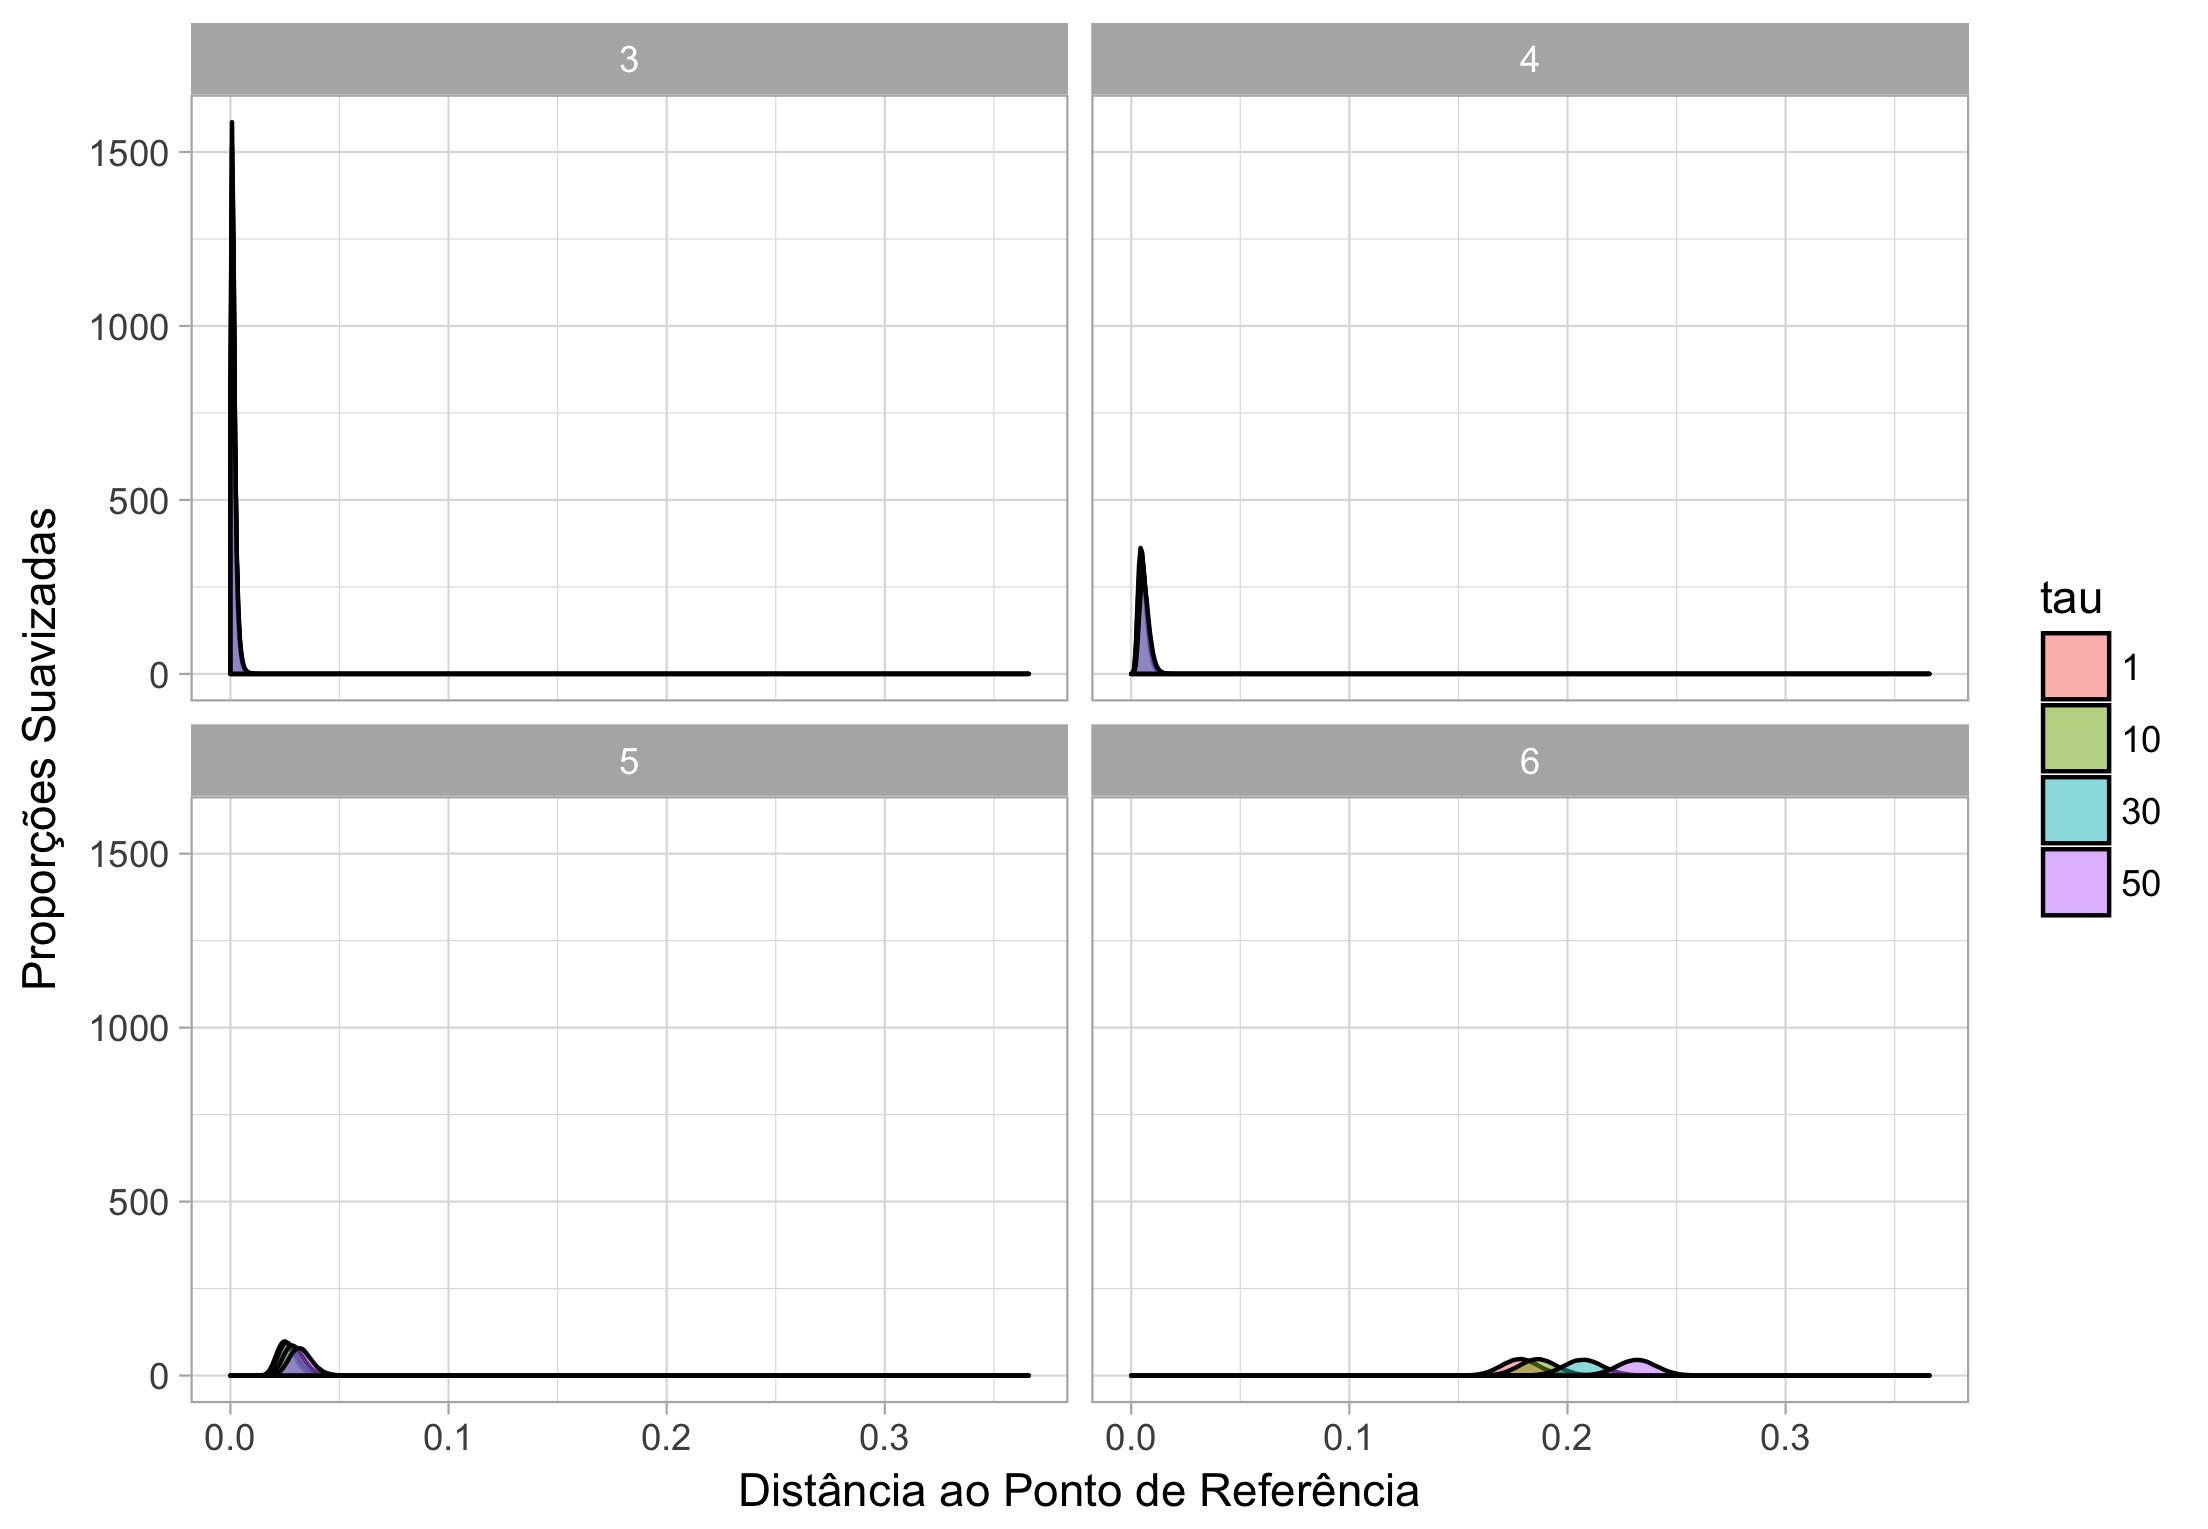
\includegraphics[width=.7\linewidth]{HistoDistanciasAleat}
		\caption{Histogramas suavizados das distâncias euclidianas dos padrões ao ponto de referência, para $D\in\{3,4,5,6\}$ e $\tau\in\{1,10,30,50\}$.}\label{Fig:HistoDistanciasAleat}
	\end{figure}
\end{block}
\end{frame}

\begin{frame}{Resultados}{}
\begin{block}{}
	Da análise aqui apresentada concluímos que, à luz da distância do ponto característico de uma sequência ao ponto de referência, os dois geradores físicos produzem sequências indistinguíveis.
	Diante disso, nos cálculos subsequentes faremos a junção desses conjuntos de dados, que denominaremos simplesmente ``aleatórios'' no que segue.
\end{block}
\end{frame}

%-------------------------------------------------------
\subsection{Análise das regiões de confiança}
%-------------------------------------------------------
\begin{frame}{Resultados}{Análise das regiões de confiança}
\begin{block}{Sequências ``Aleatórias''}
	Feita a junção das distâncias dos pontos característicos ao ponto de referência das sequências produzidas pelos geradores quântico e de rádio (sequências aleatórias), 
	para cada situação de $N$=($1.000$, $50.000$), $D$=($3$, $4$, $5$, $6$) e $\tau$=($1$, $10$, $30$, $50$), o próximo passo consiste em calcular os quantis relevantes.
	
	\pause
	Inicialmente ilustraremos apenas duas situações.
	As figuras subsequentes mostram os padrões das sequências aleatórias para o caso $N$=$1.000$, $D$=$3$, $\tau$=$1$ e para o caso $N$=$50.000$, $D$=$6$, $\tau$=$50$ no plano Entropia-Complexidade, junto com os quantis de \SI{90}{\percent}, \SI{95}{\percent}, \SI{99}{\percent} e \SI{99,9}{\percent} em escala linear e em escala logarítmica.
\end{block}
\end{frame}

\begin{frame}{Resultados}{Análise das regiões de confiança}
	\begin{block}{Análise das regiões de confiança}
		Nestas figuras, os pontos característicos foram desenhados com um gradiente de cores que vai do amarelo ao preto em função da distância ao ponto de referência.
		Identificamos também os valores de Entropia e de Complexidade Estatística correspondentes a cada quantil de interesse, estes últimos plotados em vermelho.
	\end{block}
\end{frame}

\begin{frame}{Resultados}{Análise das regiões de confiança}
\begin{block}{Análise das regiões de confiança}
	\begin{figure}
		\centering
		\subfigure[Escala linear\label{Fig:scatter1000D3t1}]{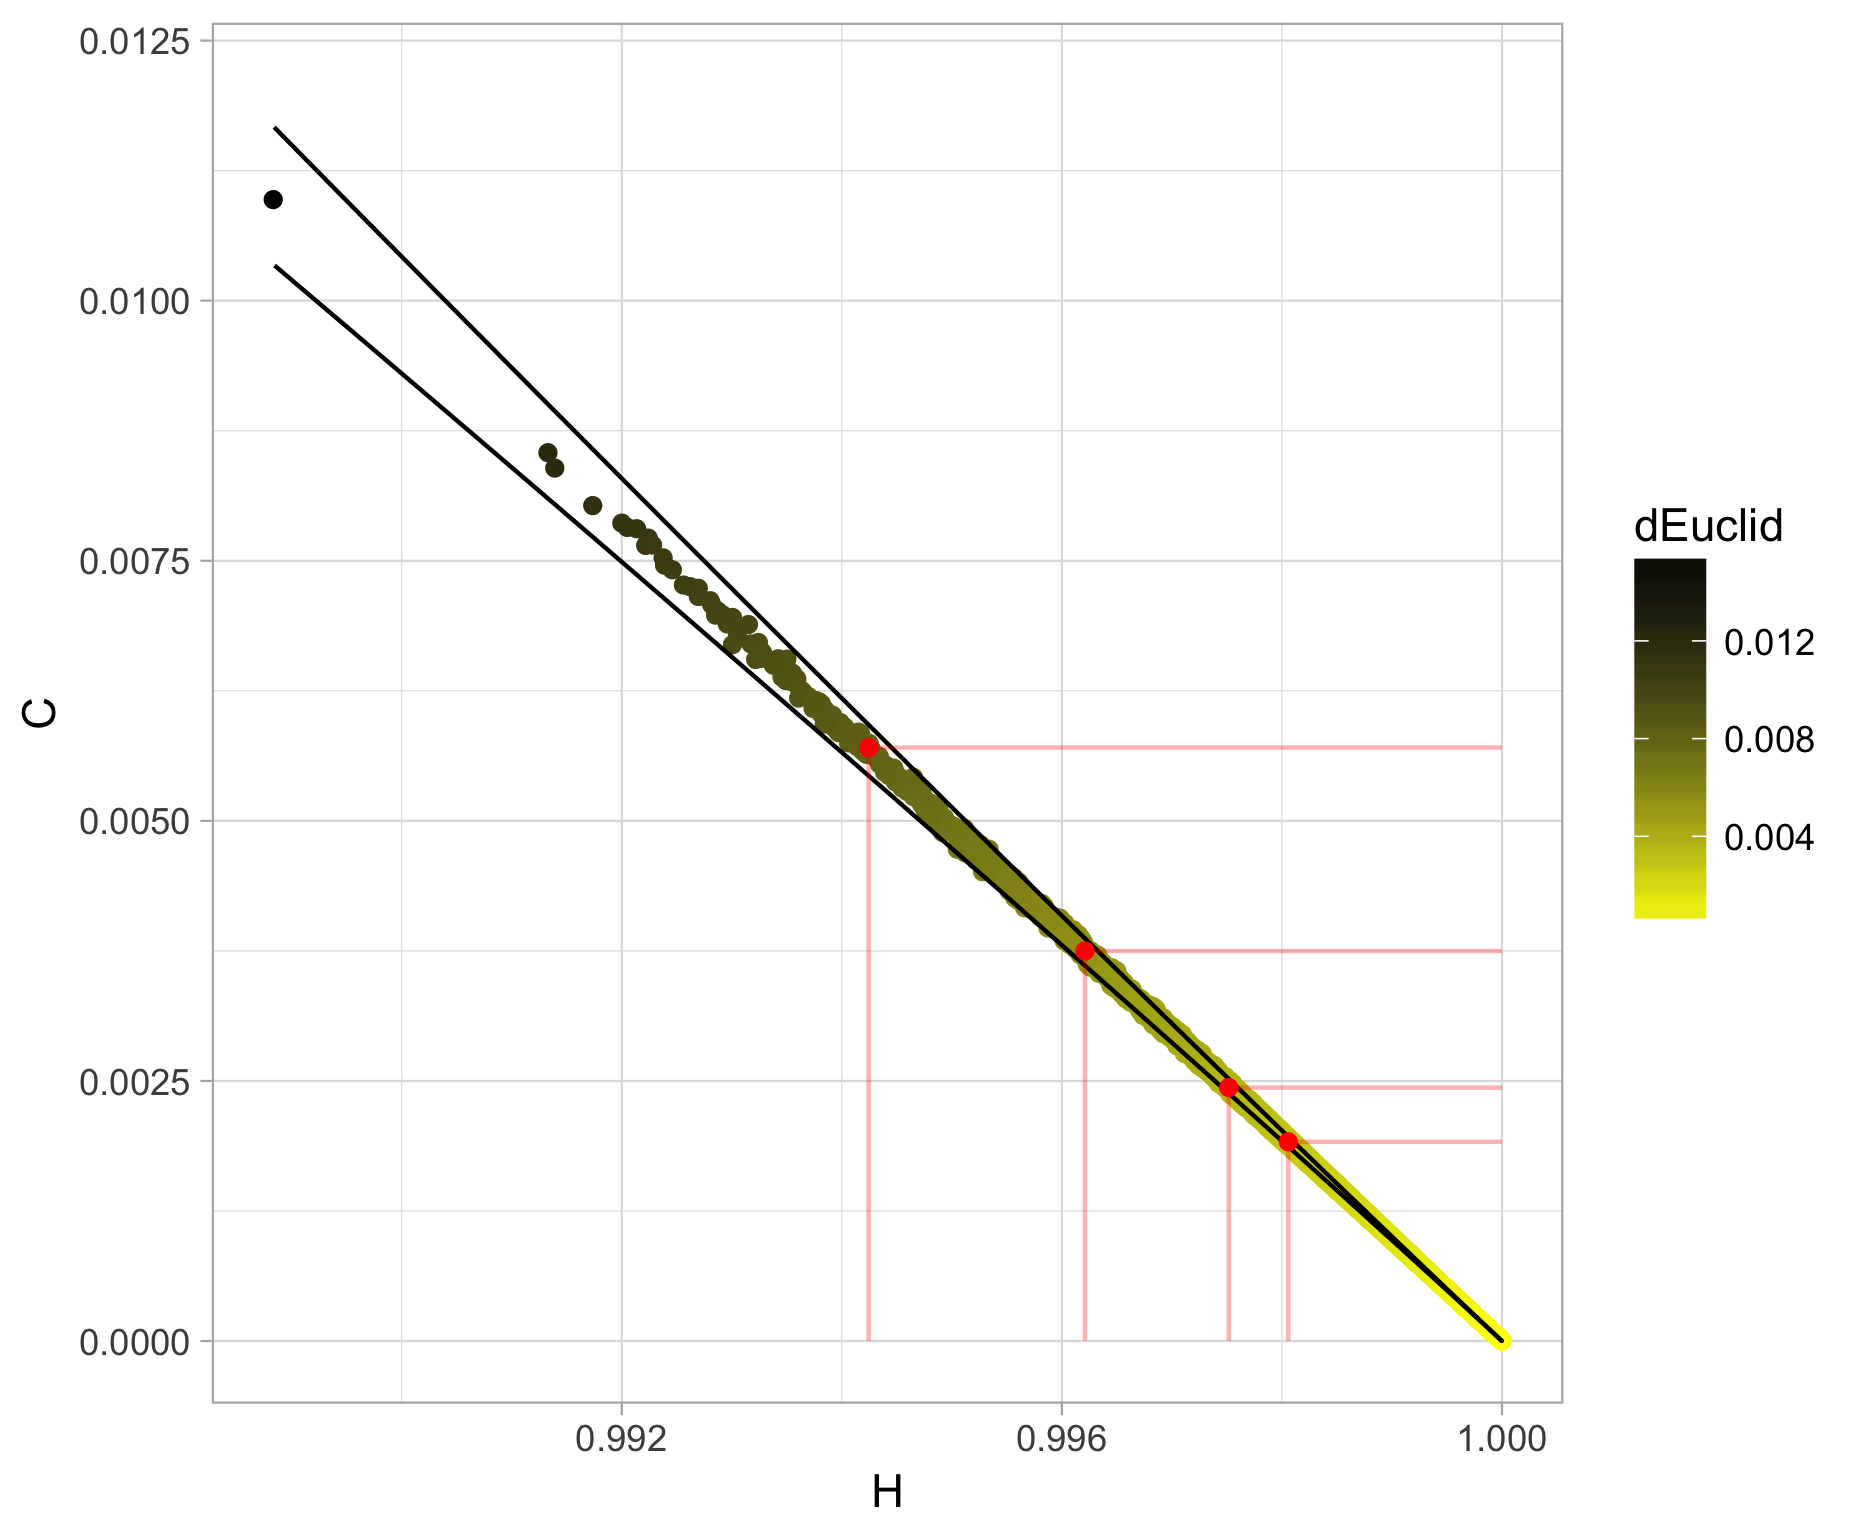
\includegraphics[width=.48\linewidth]{scatter1000D3t1}}
		\subfigure[Escala logarítmica\label{Fig:scatter1000D3t1_log}]{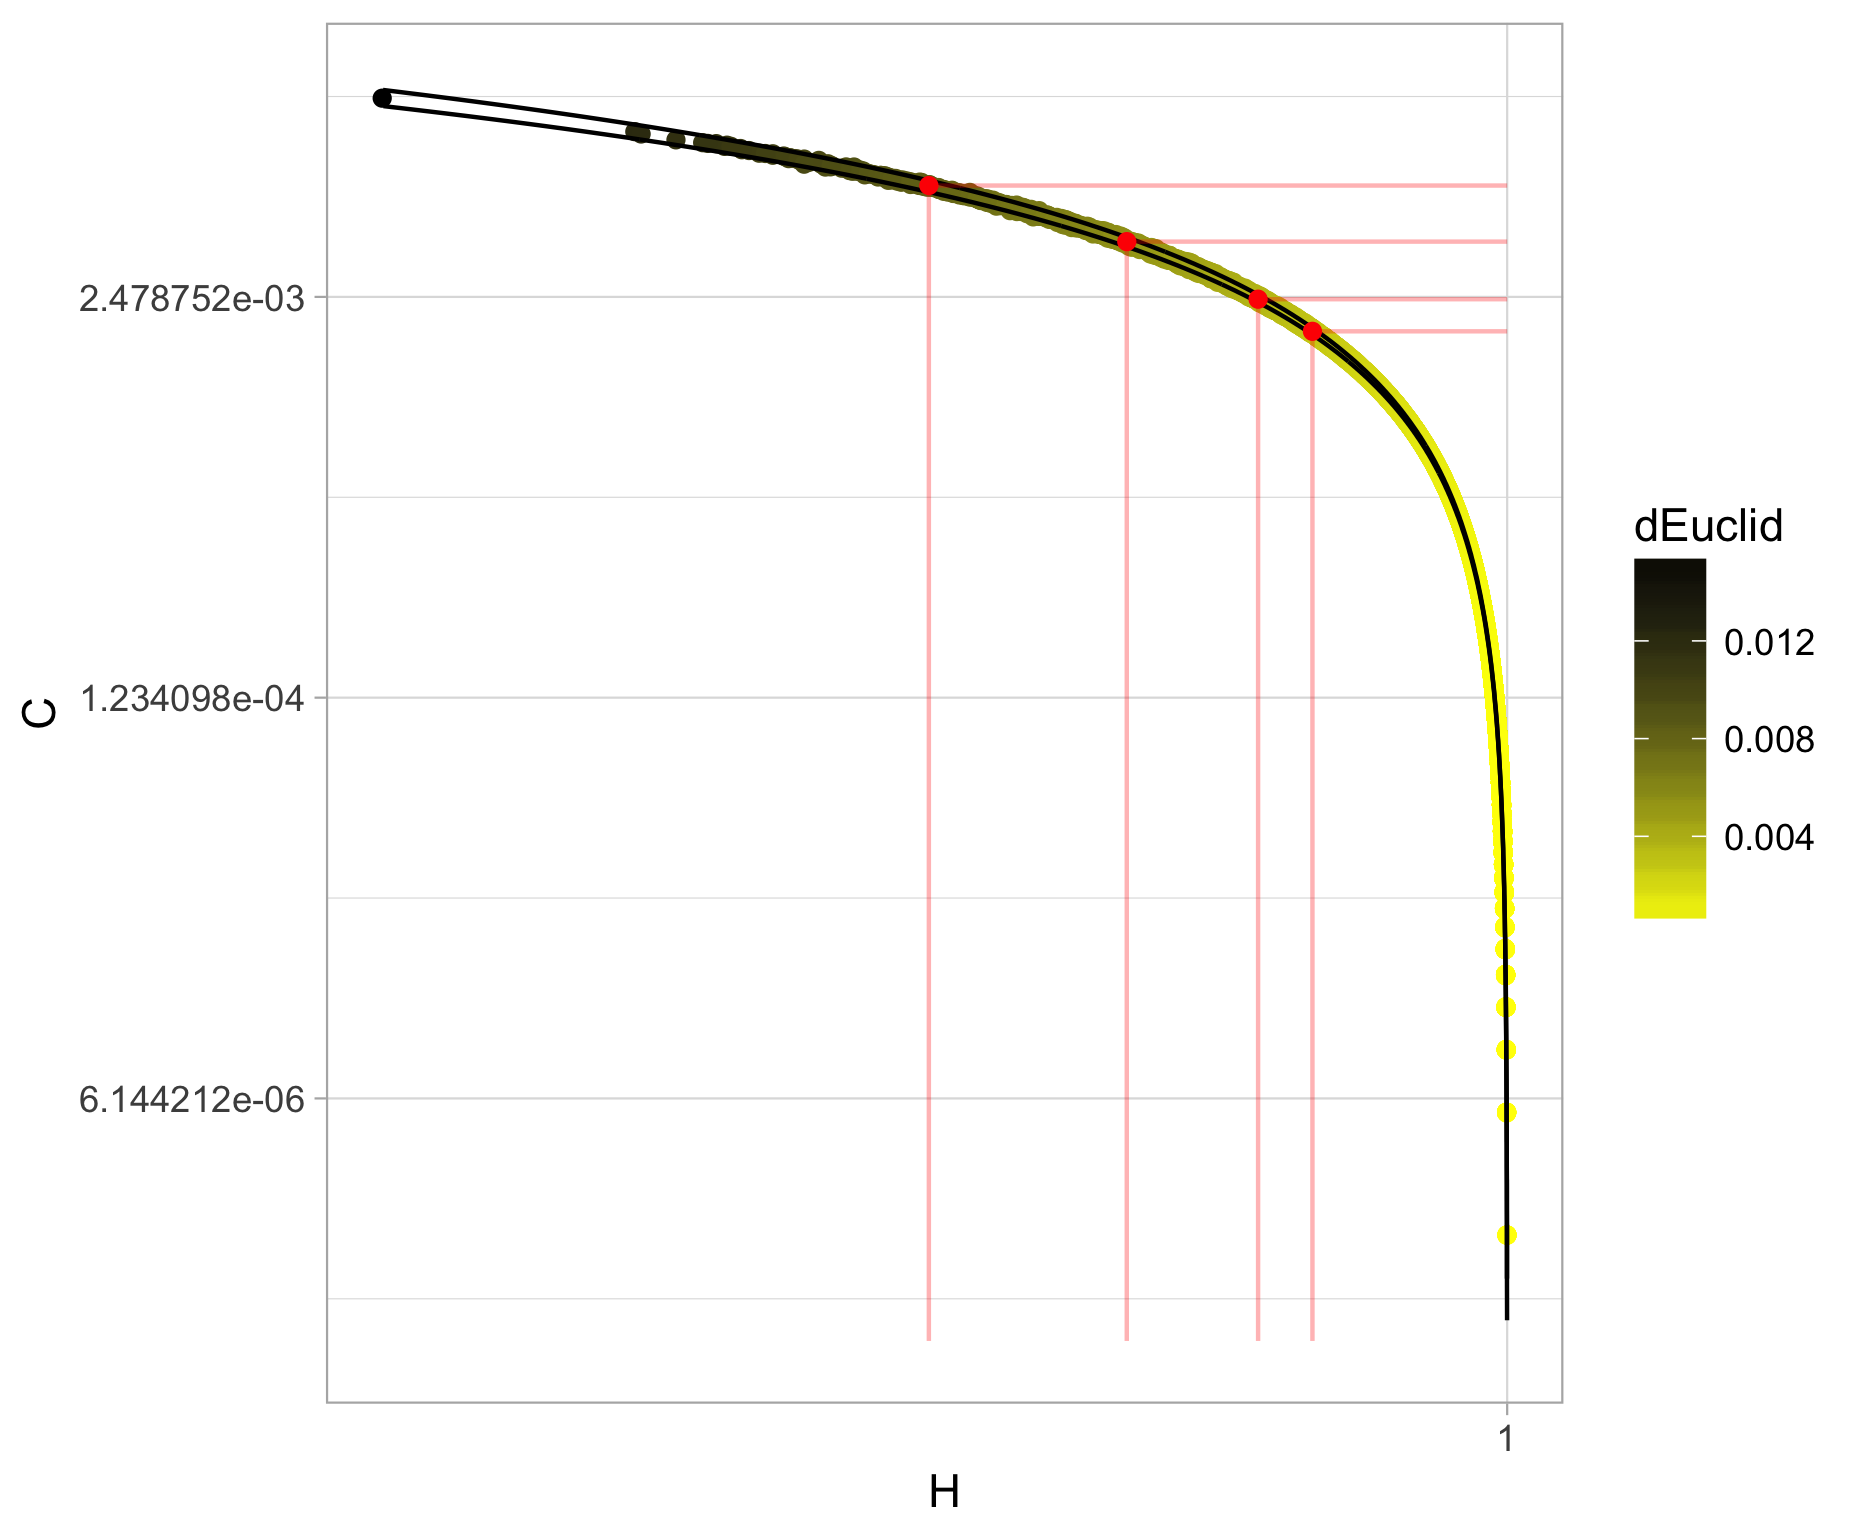
\includegraphics[width=.48\linewidth]{scatter1000D3t1_log}}
		\caption{Diagramas de dispersão das sequências aleatórias para o caso $N=1.000$, $D=3$ e $\tau=1$.}\label{Fig:AleattD3tau1}
	\end{figure}	
\end{block}
\end{frame}

\begin{frame}{Resultados}{Análise das regiões de confiança}
\begin{block}{Análise das regiões de confiança}
	\begin{figure}
		\centering
		\subfigure[Escala linear\label{Fig:scatter50kD6t50}]{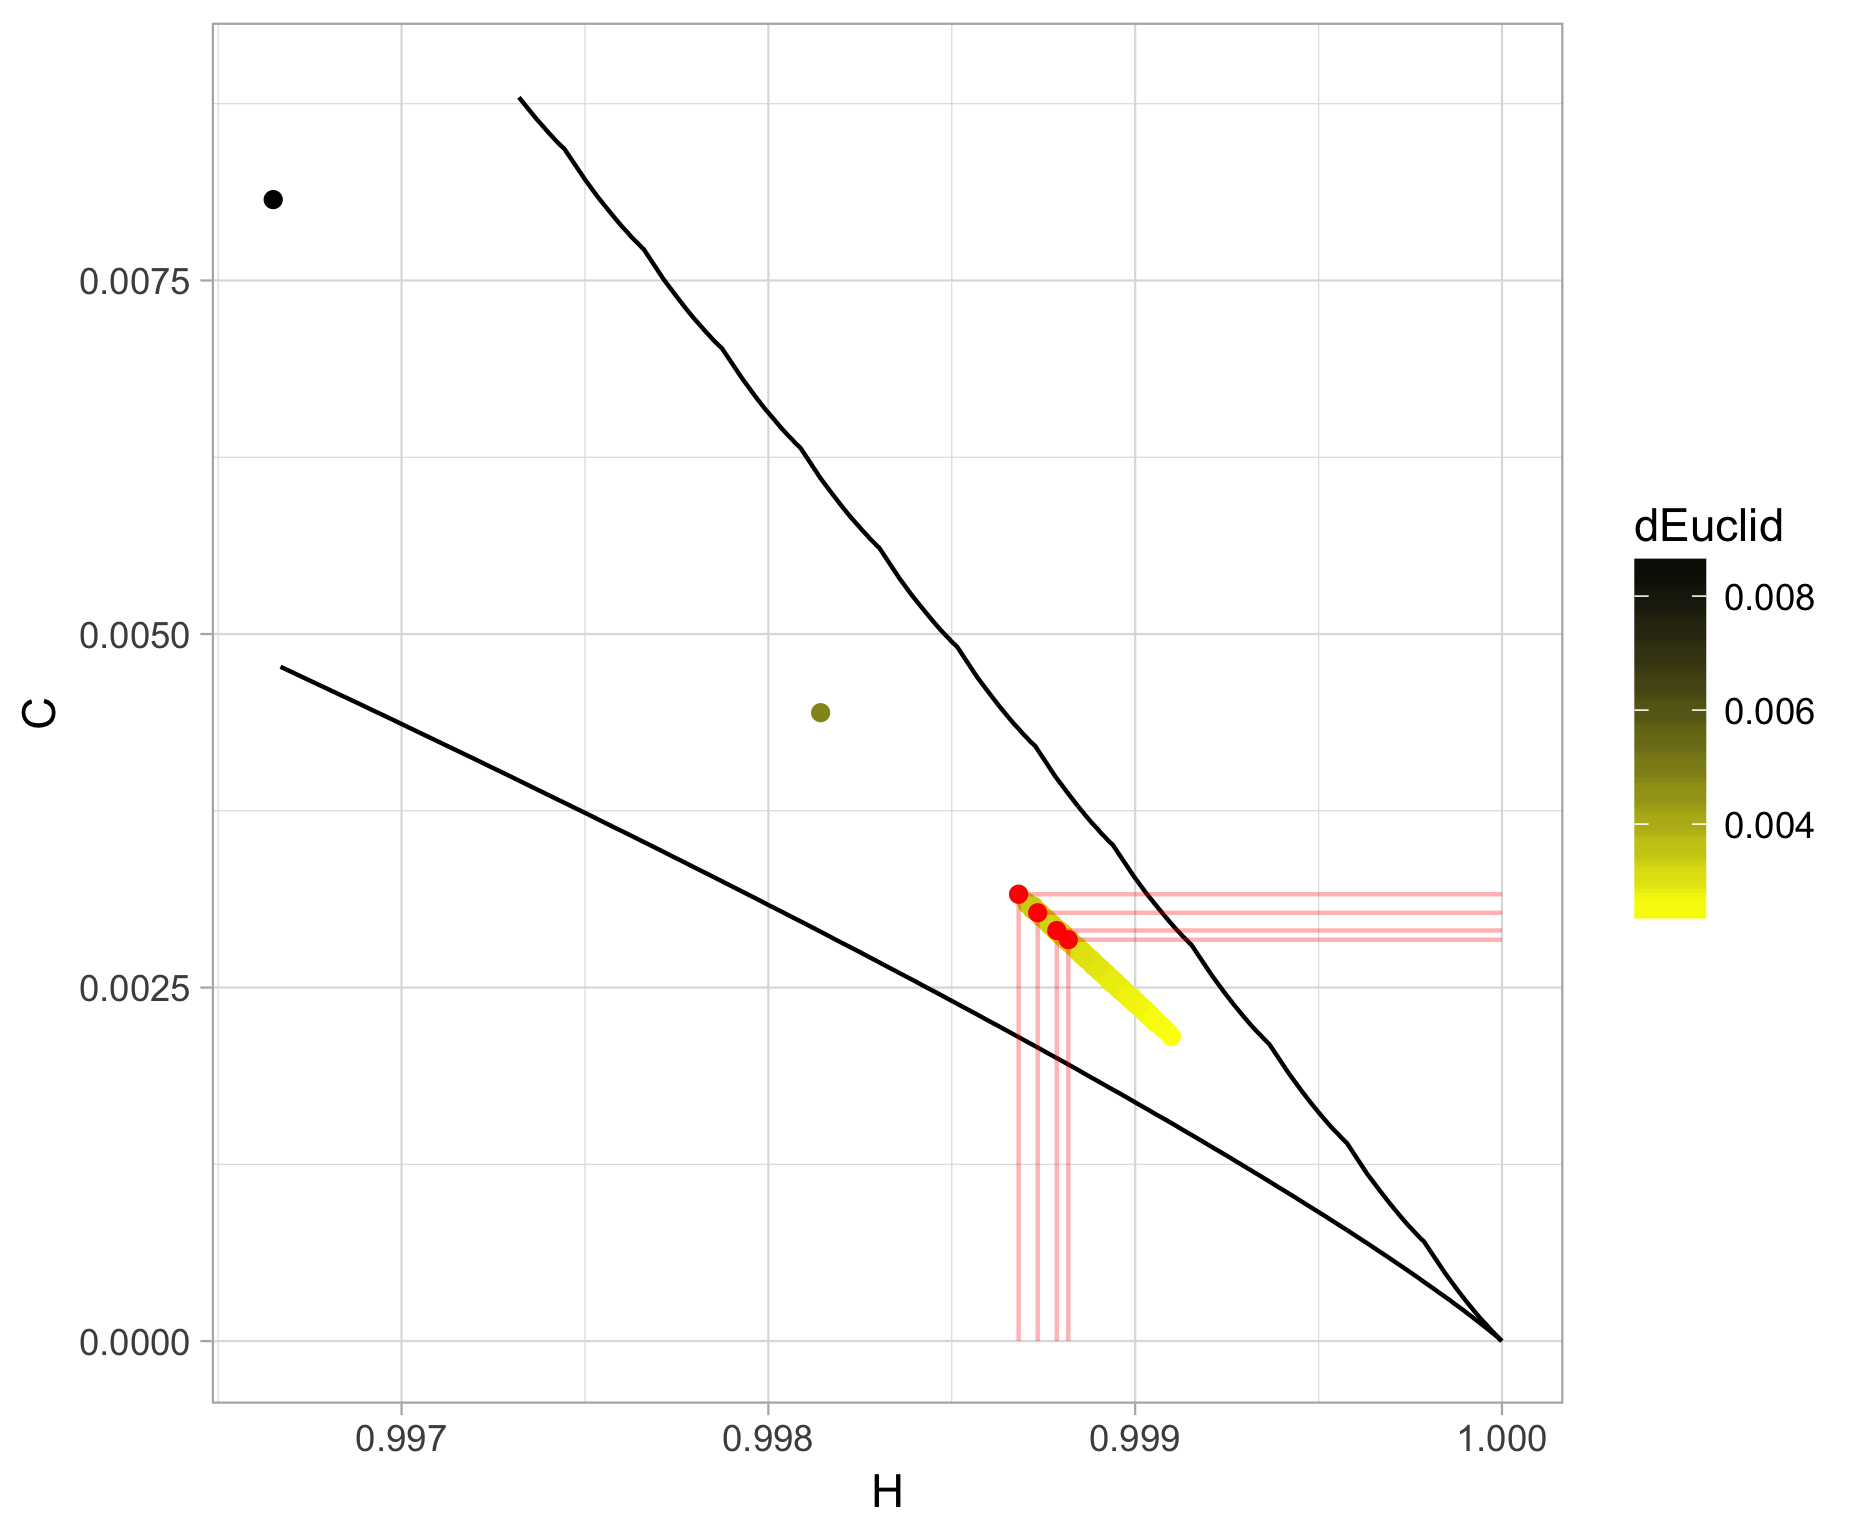
\includegraphics[width=.48\linewidth]{scatter50kD6t50}}
		\subfigure[Escala logarítmica\label{Fig:scatter50kD6t50_log}]{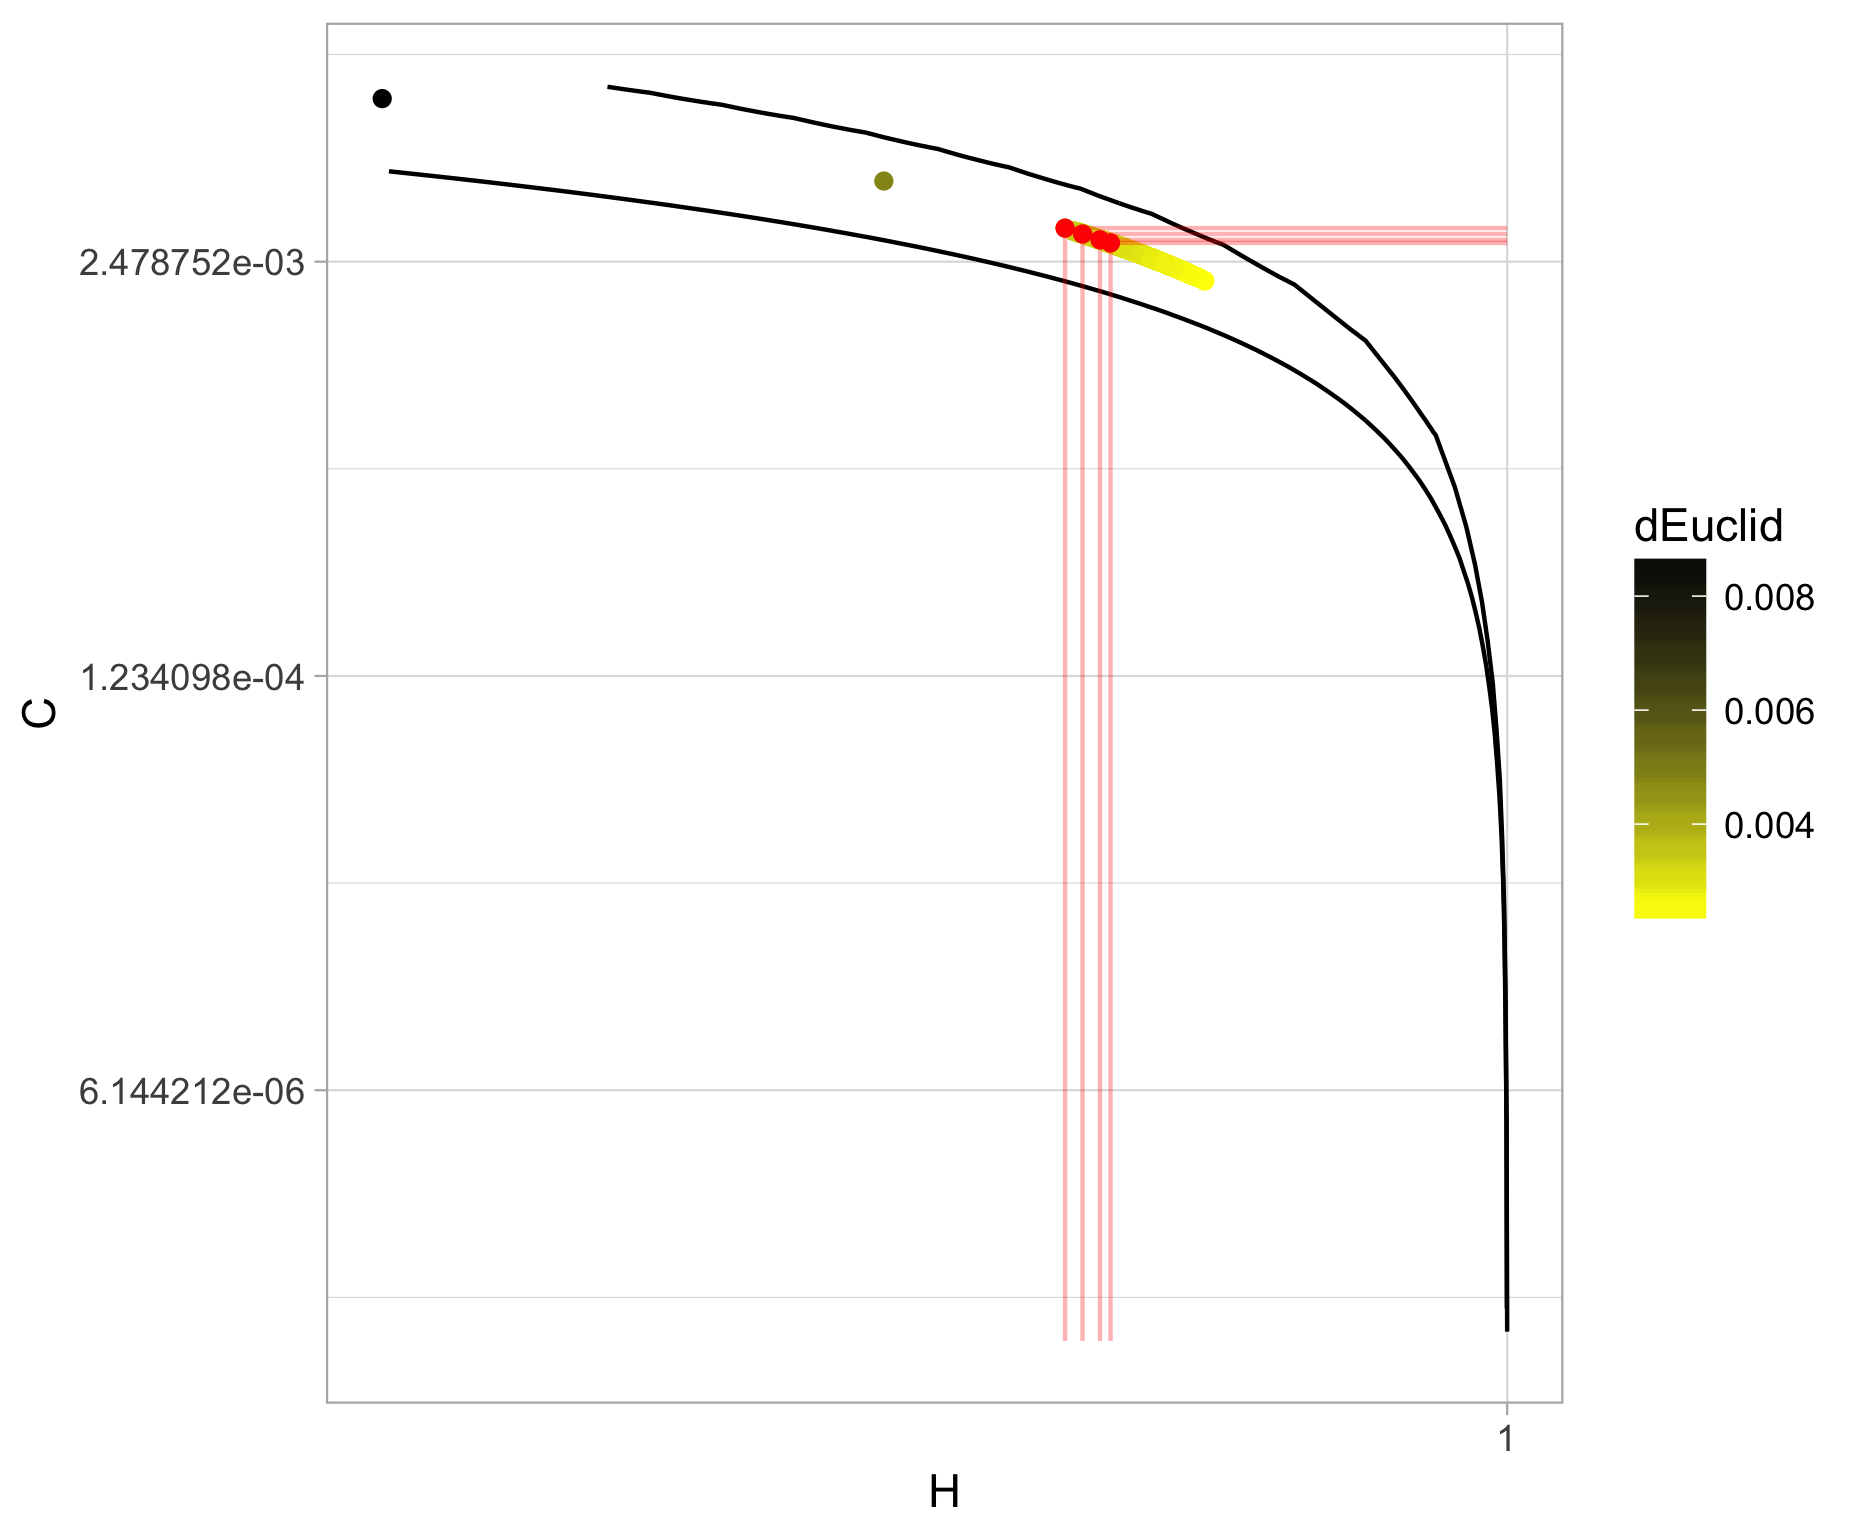
\includegraphics[width=.48\linewidth]{scatter50kD6t50_log}}
		\caption{Diagramas de dispersão das sequências aleatórias para o caso $N=50.000$, $D=6$ e $\tau=50$.}\label{Fig:QuantD3tau10log}
	\end{figure}
\end{block}
\end{frame}

\begin{frame}{Resultados}{Análise das regiões de confiança}
\begin{block}{Análise das regiões de confiança}
As figuras a seguir apresentam os resultados centrais dessa dissertação, nelas exibimos os quantis de interesse para amostras de tamanho $1.000$ e $\tau$=($1$, $10$, $30$, $50$), logo em seguida para amostras de tamanho $50.000$ e, assim como anteriormente, $\tau$=($1$, $10$, $30$, $50$).
Cada uma destas figuras inclui as quatro situações de $D$=($3$, $4$, $5$, $6$).\\
\pause
Adicionalmente aos gráficos são apresentadas tabelas, mostrando os valores da distância euclidiana dos pontos de interesse dos quantis ao ponto de referência.
\end{block}
\end{frame}

%% 1k ============
\begin{frame}{Resultados}{Análise das regiões de confiança}
\begin{block}{$N=1.000$ e $\tau=1$}
	\begin{figure}
		\centering
		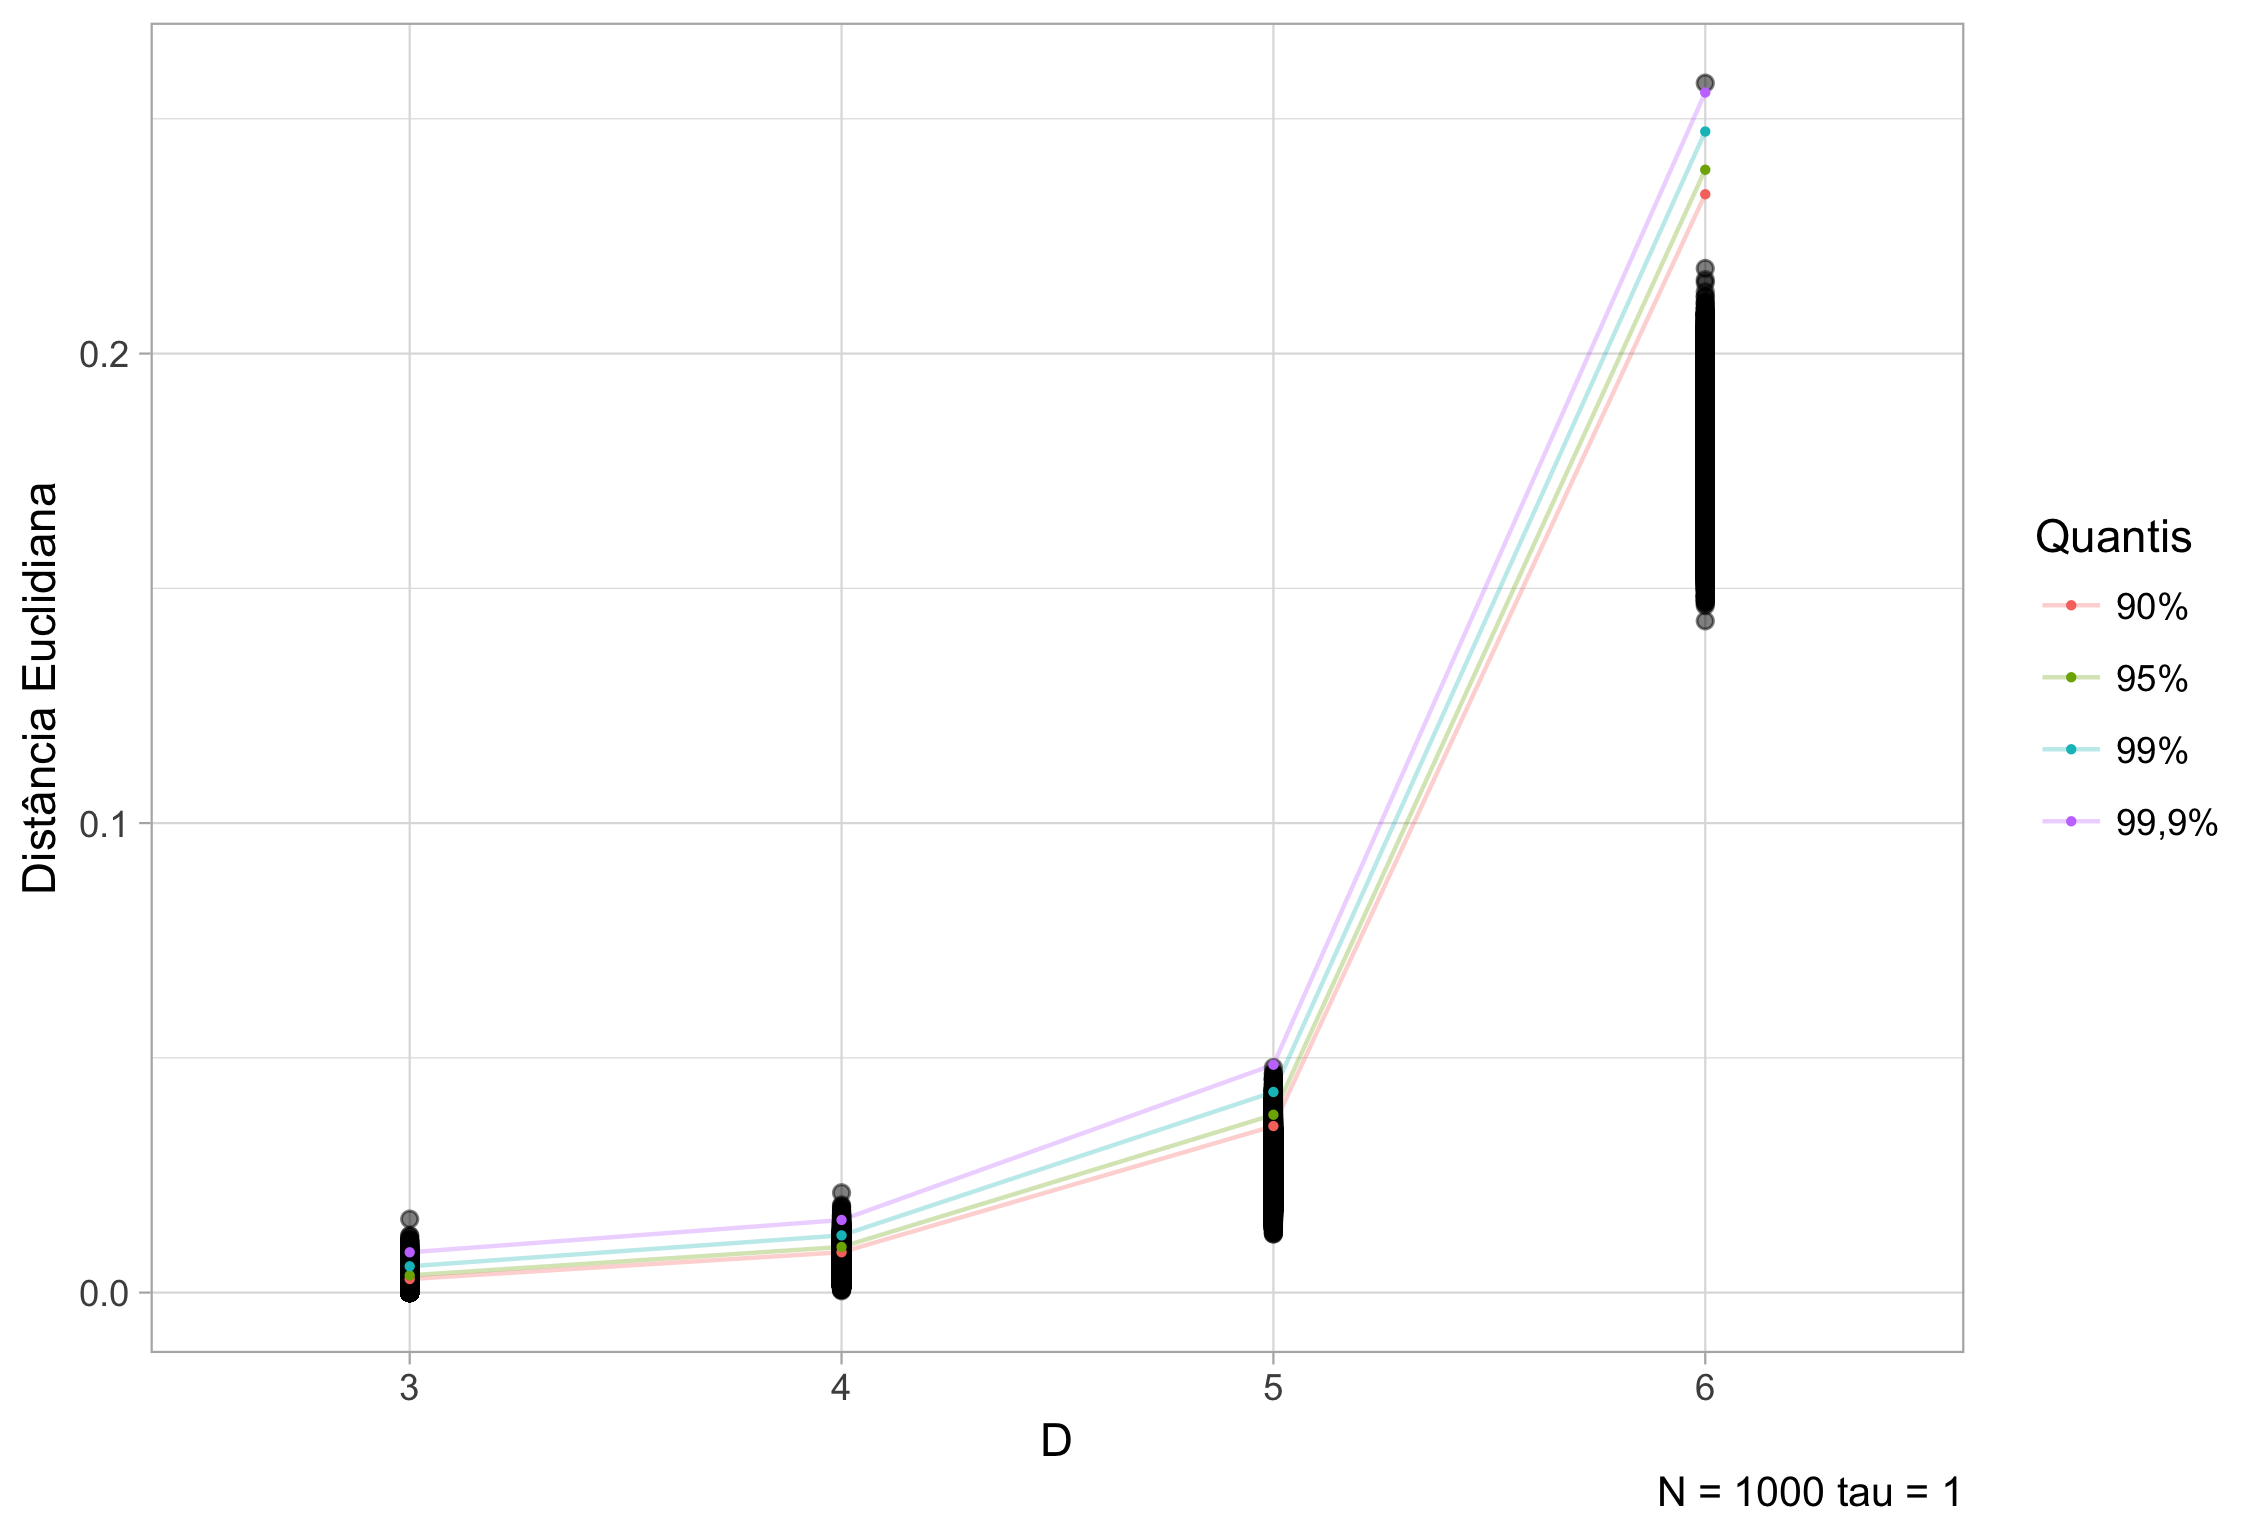
\includegraphics[width=.7\linewidth]{Conf_Int_1k_T1_noMT}
		\caption{Intervalos de confiança para o caso $N=1.000$ e $\tau=1$.}\label{Fig:Conf_Int_1k_T1}
	\end{figure}
	
\end{block}
\end{frame}

\begin{frame}{Resultados}{Análise das regiões de confiança}
	\begin{block}{$N=1.000$ e $\tau=10$}
	\begin{figure}
		\centering
		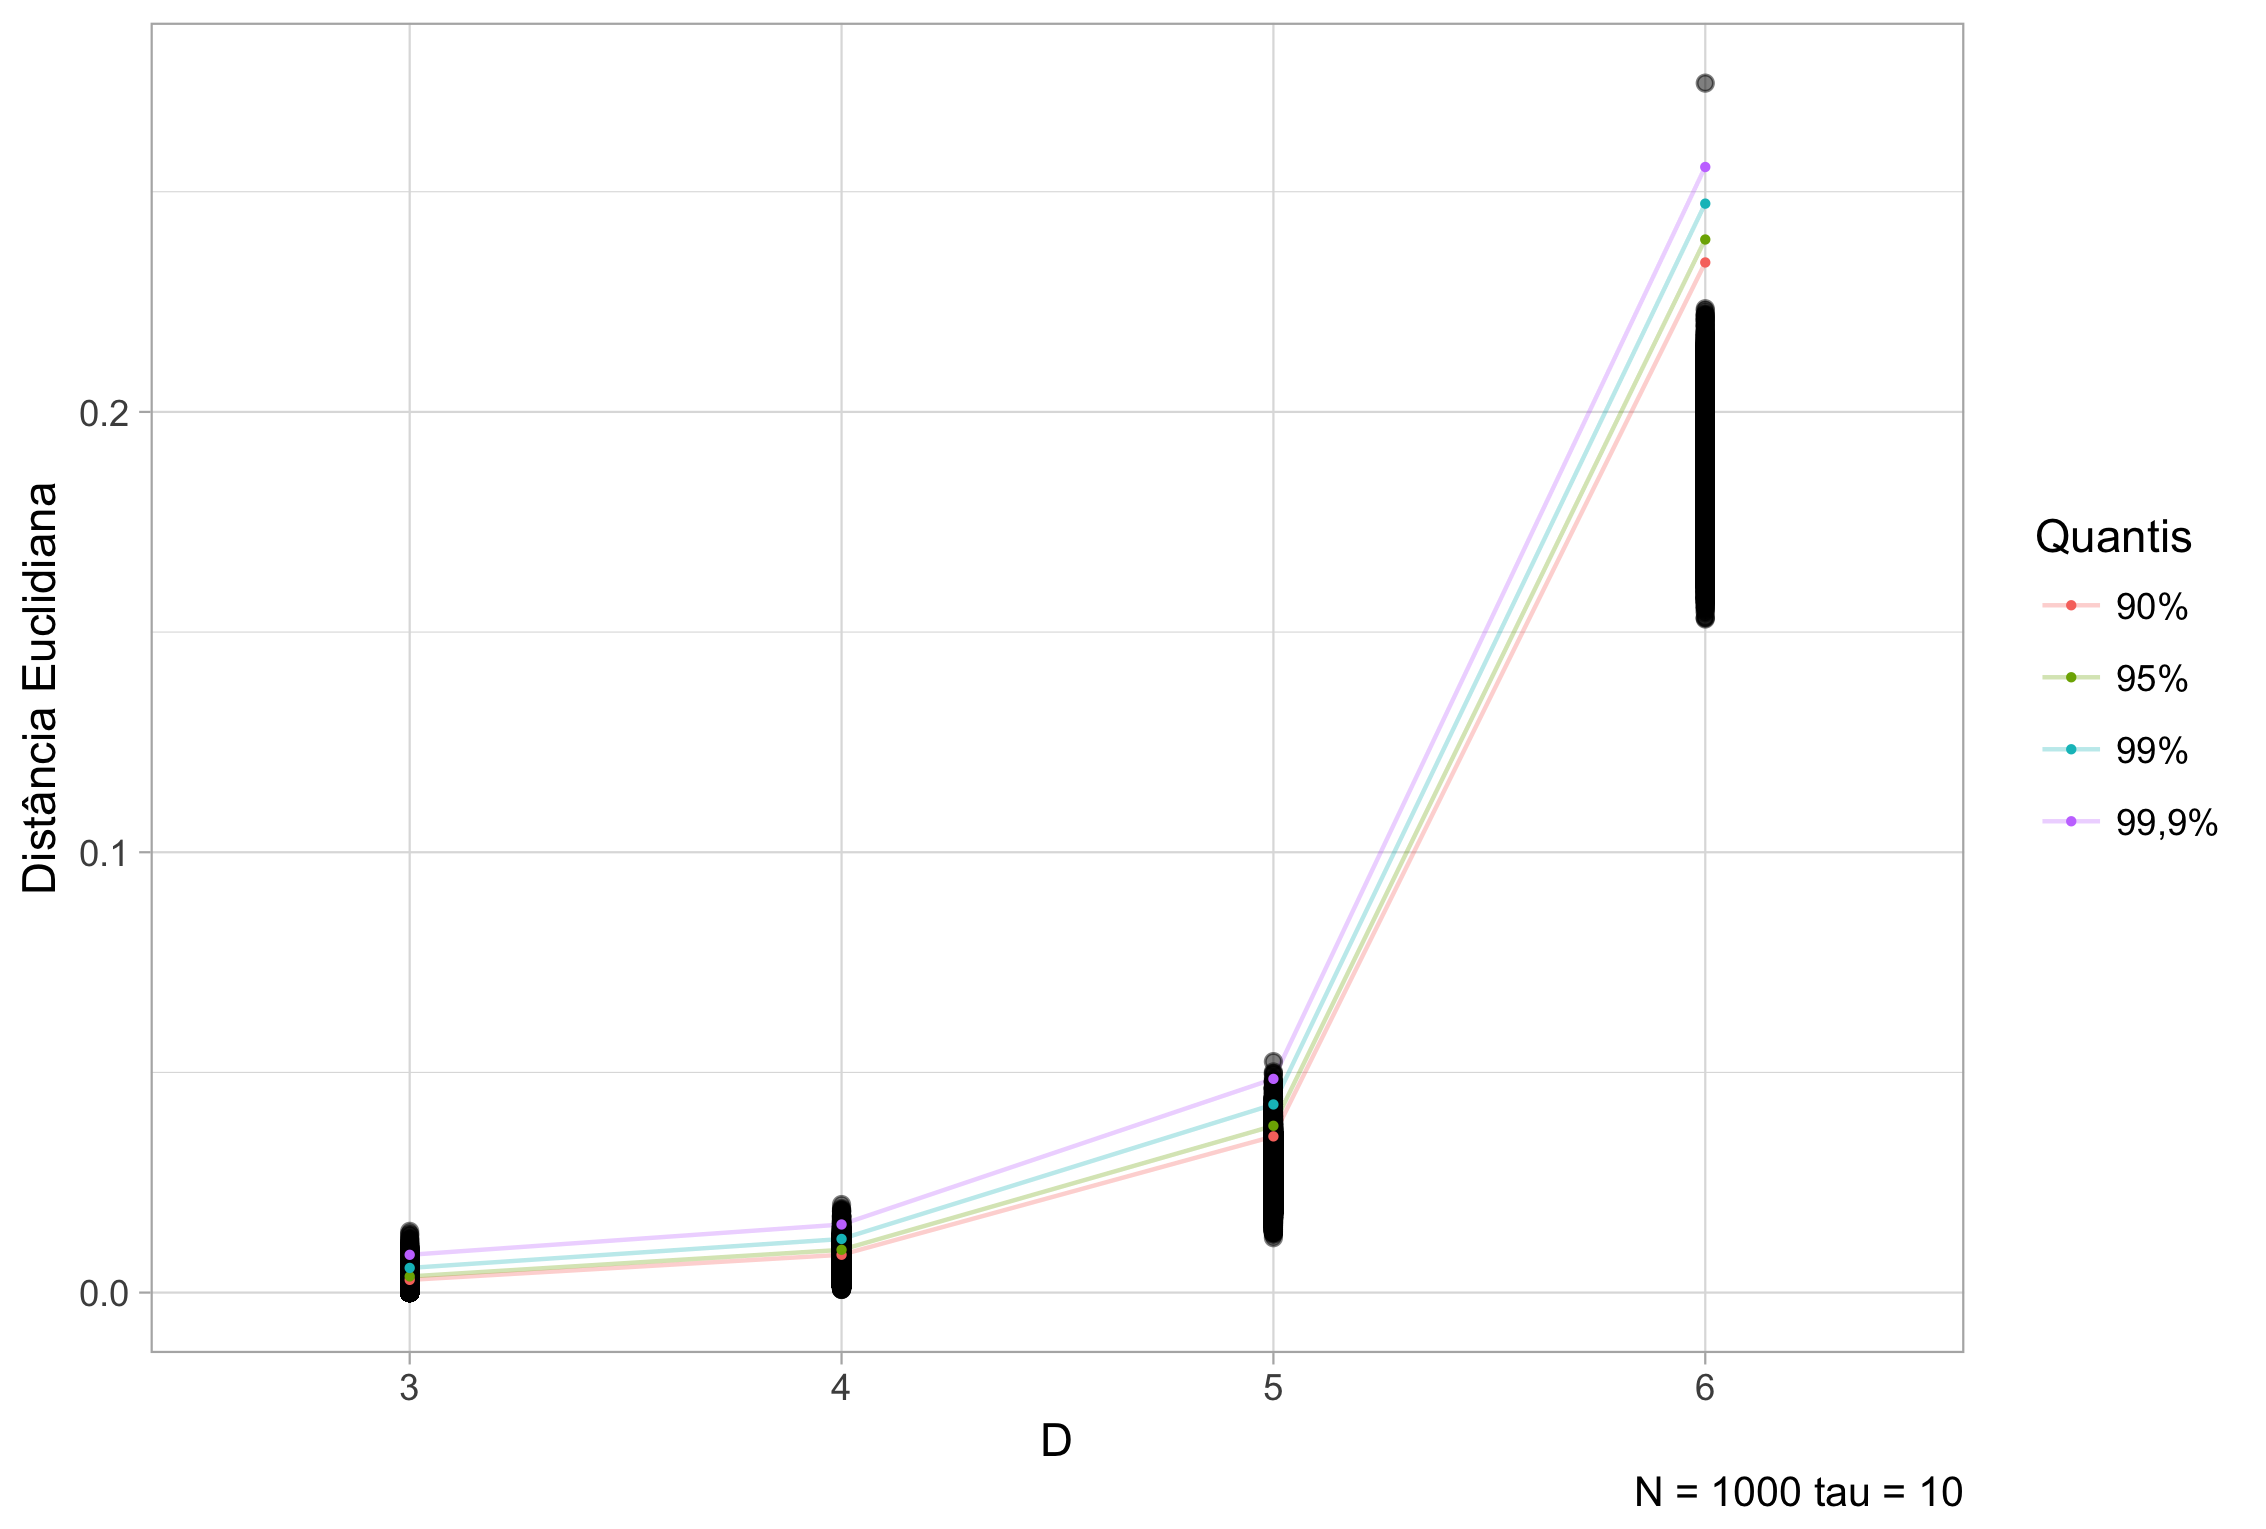
\includegraphics[width=.7\linewidth]{Conf_Int_1k_T10_noMT}
		\caption{Intervalos de confiança para o caso $N=1.000$ e $\tau=10$.}\label{Fig:Conf_Int_1k_T10}
	\end{figure}	
	\end{block}
\end{frame}

\begin{frame}{Resultados}{Análise das regiões de confiança}
	\begin{block}{$N=1.000$ e $\tau=30$}
	\begin{figure}
		\centering
		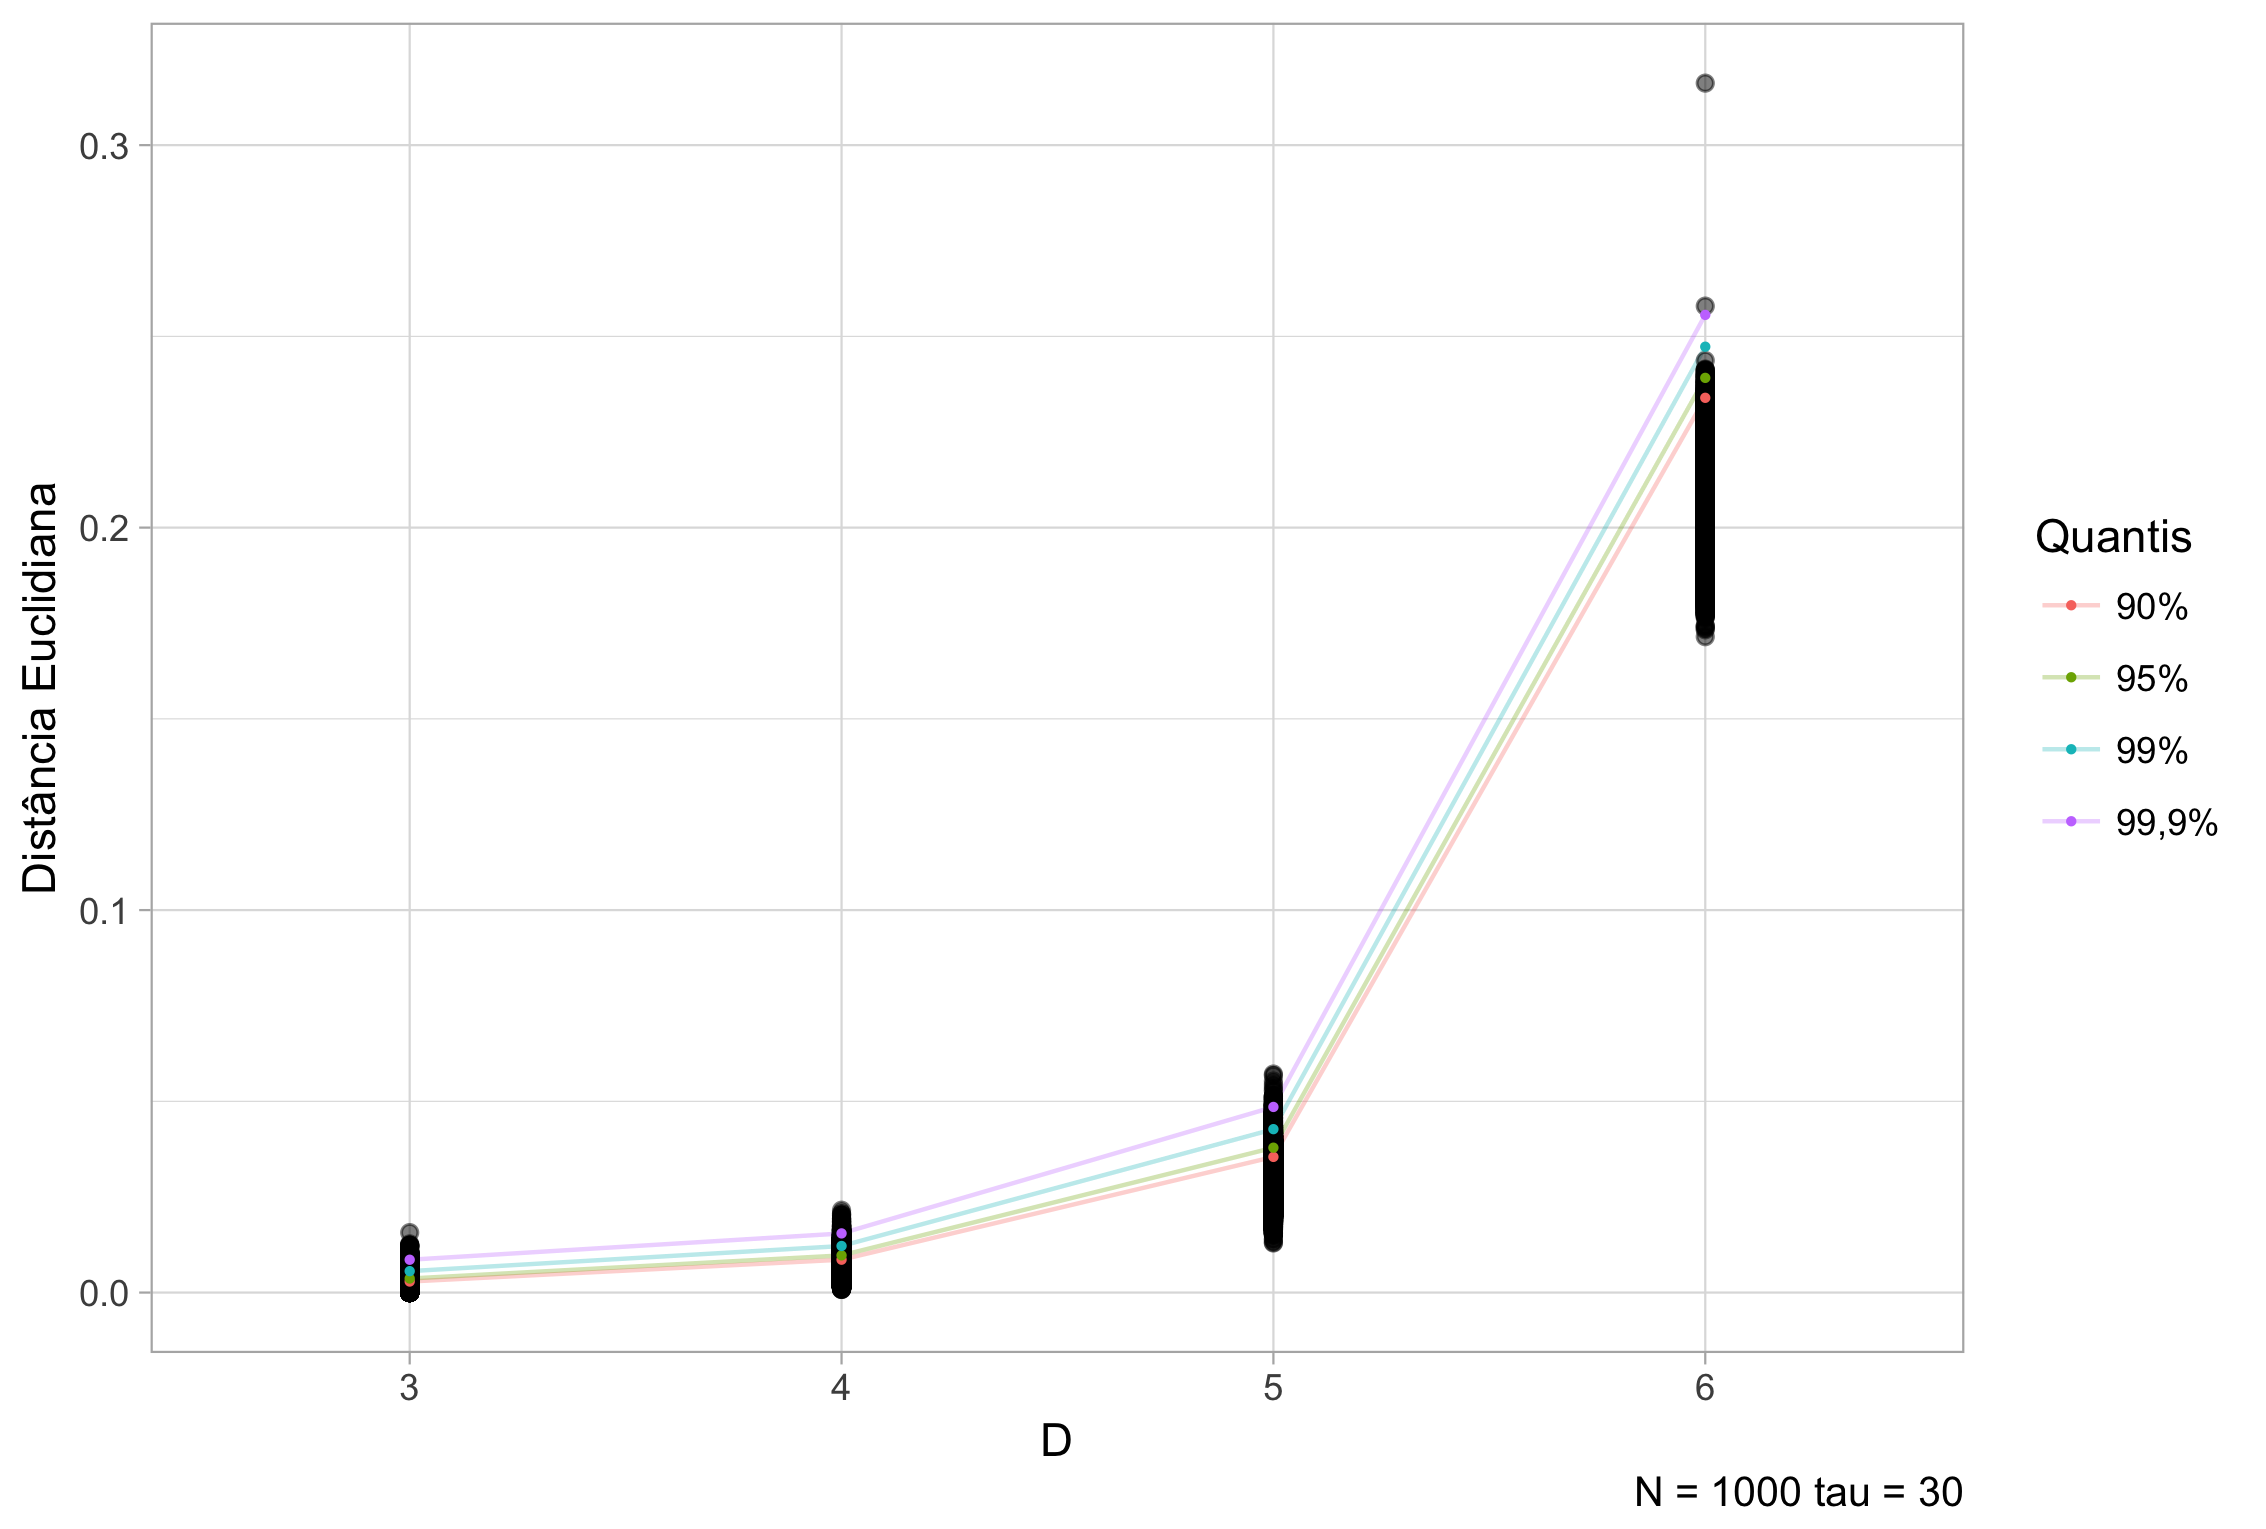
\includegraphics[width=.7\linewidth]{Conf_Int_1k_T30_noMT}
		\caption{Intervalos de confiança para o caso $N=1.000$ e $\tau=30$.}\label{Fig:Conf_Int_1k_30}
	\end{figure}
	\end{block}
\end{frame}

\begin{frame}{Resultados}{Análise das regiões de confiança}
	\begin{block}{$N=1.000$ e $\tau=50$}
	\begin{figure}
		\centering
		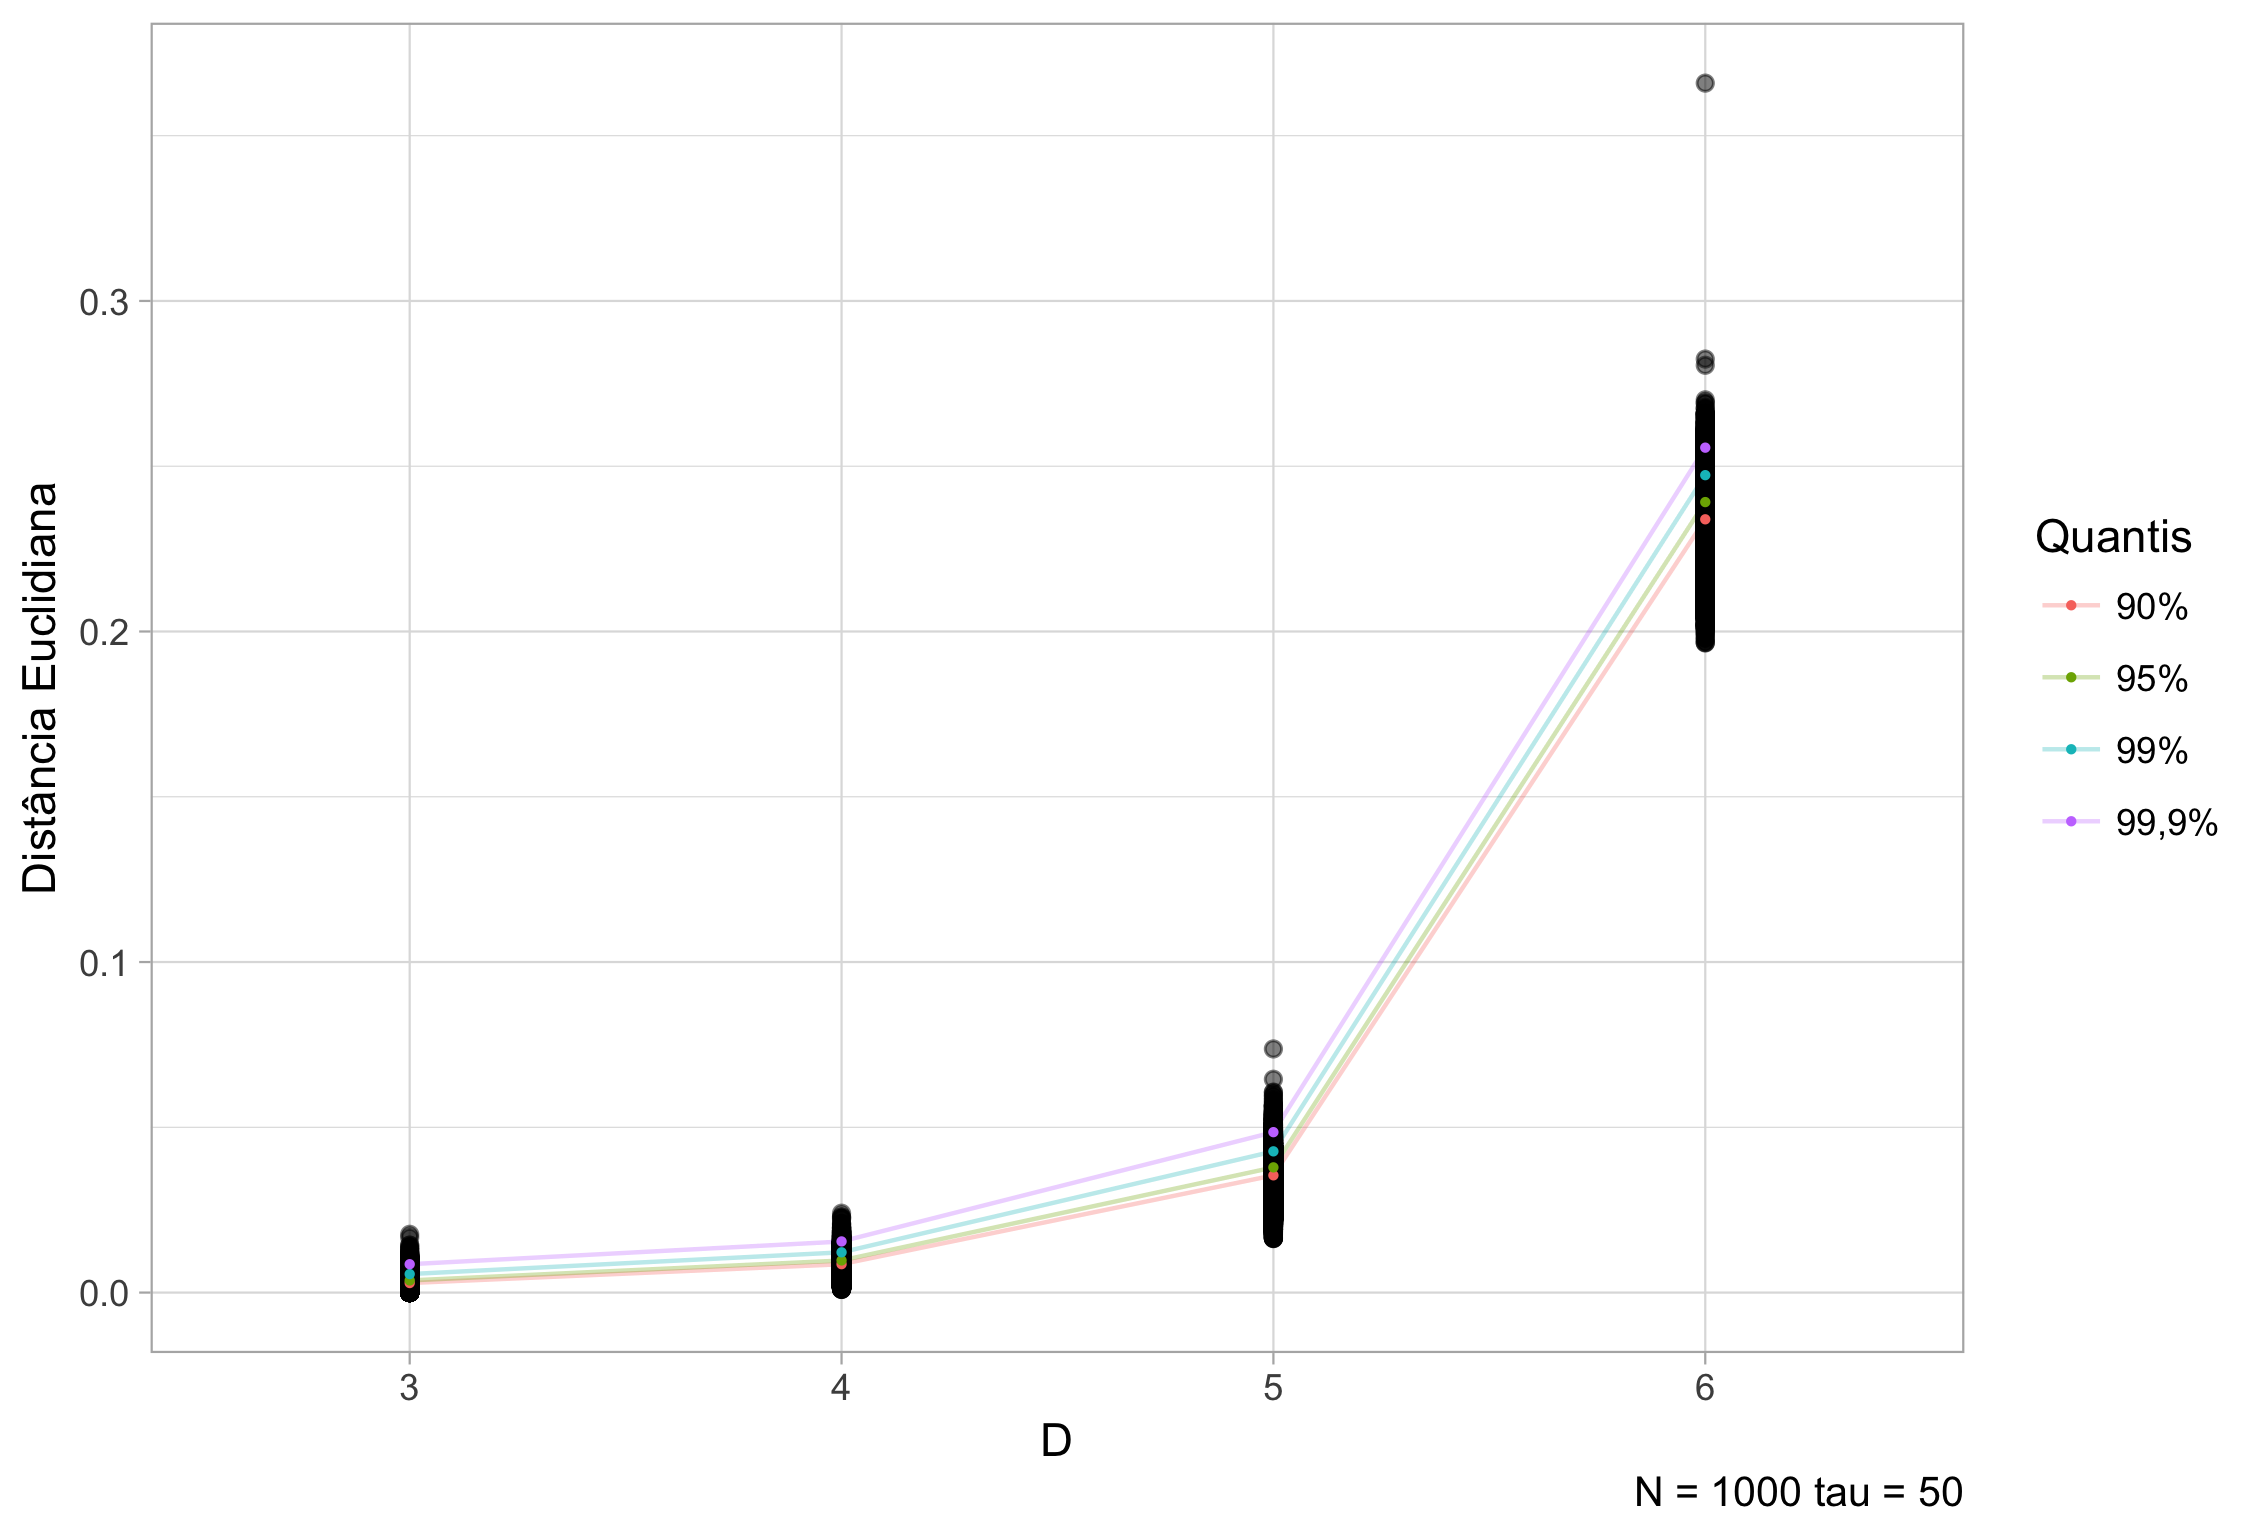
\includegraphics[width=.7\linewidth]{Conf_Int_1k_T50_noMT}
		\caption{Intervalos de confiança para o caso $N=1.000$ e $\tau=50$.}\label{Fig:Conf_Int_1k_T50}
	\end{figure}
	\end{block}
\end{frame}

\begin{frame}{Resultados}{Análise das regiões de confiança}
	\begin{block}{Quantis das distâncias, sequências de $1.000$ observações.}
		\resizebox{\linewidth}{!}{% Resize table to fit within \linewidth horizontally	
			\centering
			\begin{tabular}{ccccccc}
				\toprule
				$N=1.000$	&  $D$  &$\tau$  &\SI{90}{\percent}&\SI{95}{\percent}&\SI{99}{\percent}&\SI{99.9}{\percent}\\
				\midrule
				&  $3$ &  $ 1$ & 2.728065e-03  &  3.478919e-03  &  0.0053313857  &  0.0081048900 \\ 
				&  $3$ &  $10$ & 2.802528e-03  &  3.577539e-03  &  0.0054960059  &  0.0083091257 \\
				&  $3$ &  $30$ & 2.961344e-03  &  3.749702e-03  &  0.0056871429  &  0.0087472165 \\
				&  $3$ &  $50$ & 3.120298e-03  &  3.950138e-03  &  0.0059008109  &  0.0090272065 \\
				\midrule
				&  $4$ &  $ 1$ & 7.964076e-03  &  9.015899e-03  &  0.0112777244  &  0.0143372255 \\ 
				&  $4$ &  $10$ & 8.199472e-03  &  9.295153e-03  &  0.0116255590  &  0.0147762539 \\
				&  $4$ &  $30$ & 8.738506e-03  &  9.883617e-03  &  0.0123589751  &  0.0156235388 \\
				&  $4$ &  $50$ & 9.368242e-03  &  1.054840e-02  &  0.0131188349  &  0.0166817556 \\
				\midrule
				&  $5$ &  $ 1$ & 3.117067e-02  &  3.304803e-02  &  0.0366895915  &  0.0413215927 \\ 
				&  $5$ &  $10$ & 3.235895e-02  &  3.425898e-02  &  0.0380480169  &  0.0427998033 \\
				&  $5$ &  $30$ & 3.545788e-02  &  3.752600e-02  &  0.0417425086  &  0.0467667352 \\
				&  $5$ &  $50$ & 3.914194e-02  &  4.142425e-02  &  0.0459567507  &  0.0514563584 \\
				\midrule
				&  $6$ &  $ 1$ & 1.891794e-01  &  1.923893e-01  &  0.1984529319  &  0.2050583463 \\
				&  $6$ &  $10$ & 1.975446e-01  &  2.007669e-01  &  0.2069269144  &  0.2139321164 \\
				&  $6$ &  $30$ & 2.185870e-01  &  2.218804e-01  &  0.2280312709  &  0.2345272440 \\
				&  $6$ &  $50$ & 2.431686e-01  &  2.464034e-01  &  0.2526103765  &  0.2596196960 
%				\bottomrule
			\end{tabular}}
		\end{block}
\end{frame}

%% 50k ============

\begin{frame}{Resultados}{Análise das regiões de confiança}
	\begin{block}{$N=50.000$ e $\tau=1$}
	\begin{figure}
		\centering
		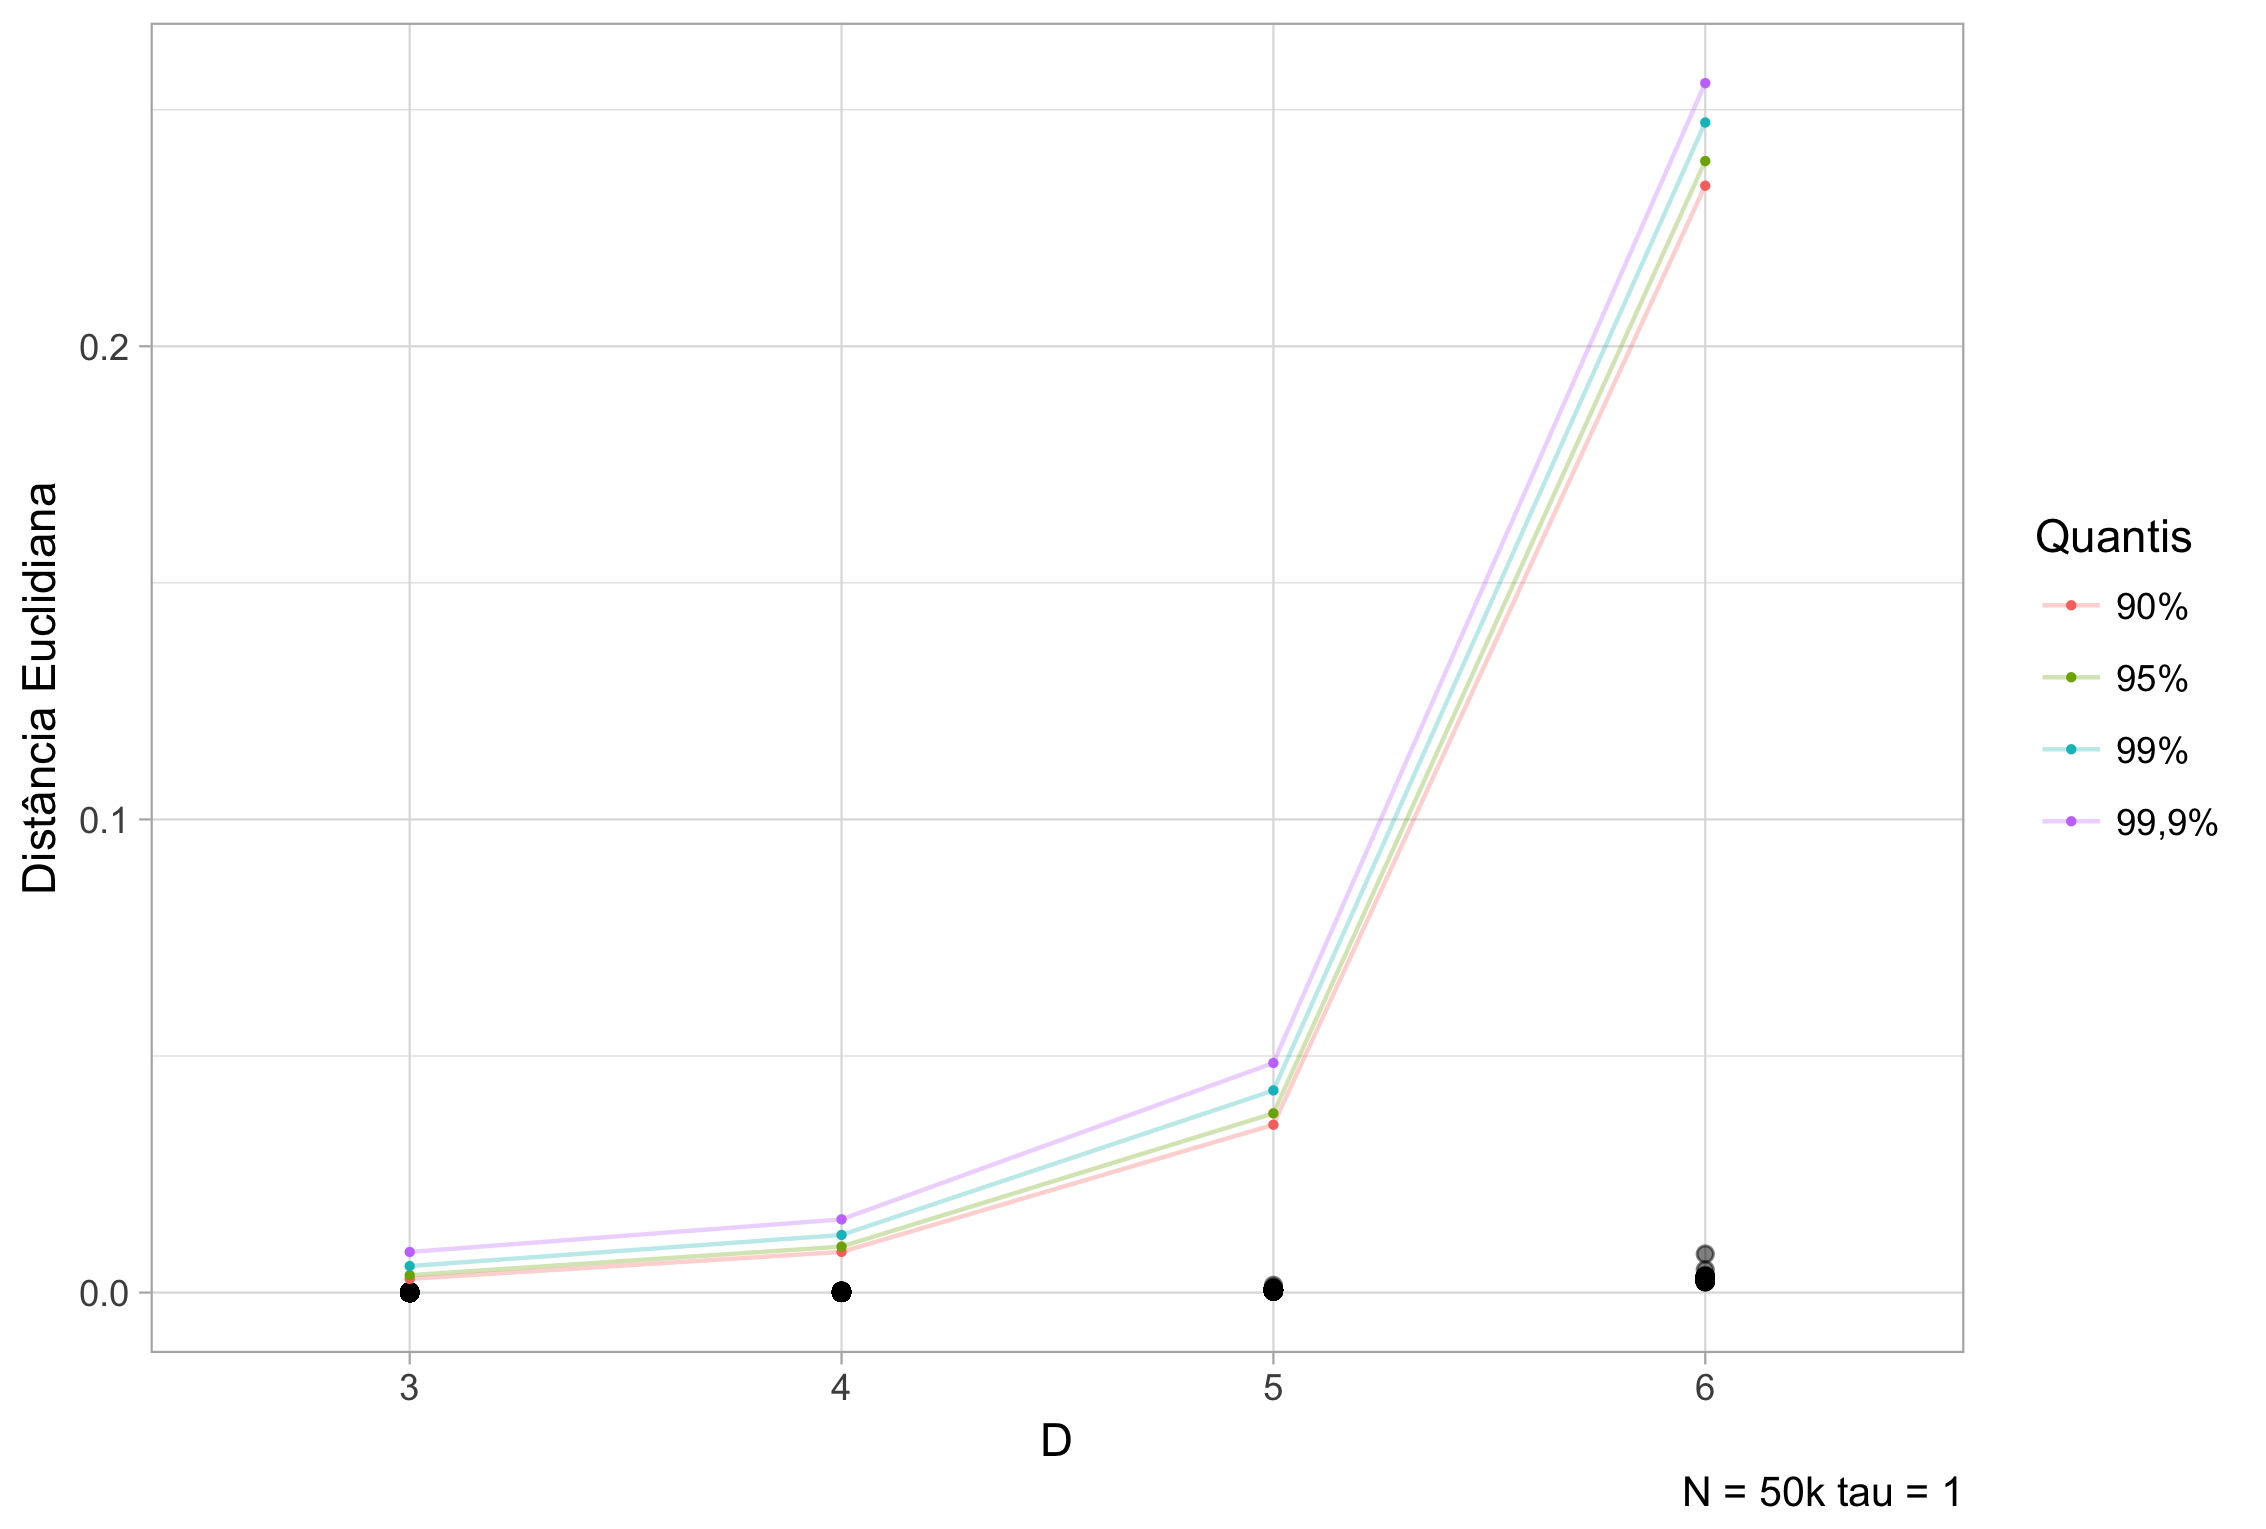
\includegraphics[width=.7\linewidth]{Conf_Int_50k_T1_noMT}
		\caption{Intervalos de confiança para o caso $N=50.000$ e $\tau=1$.}\label{Fig:Conf_Int_50k_T1}
	\end{figure}	
	\end{block}
\end{frame}

\begin{frame}{Resultados}{Análise das regiões de confiança}
	\begin{block}{$N=50.000$ e $\tau=10$}
		\begin{figure}
		\centering
		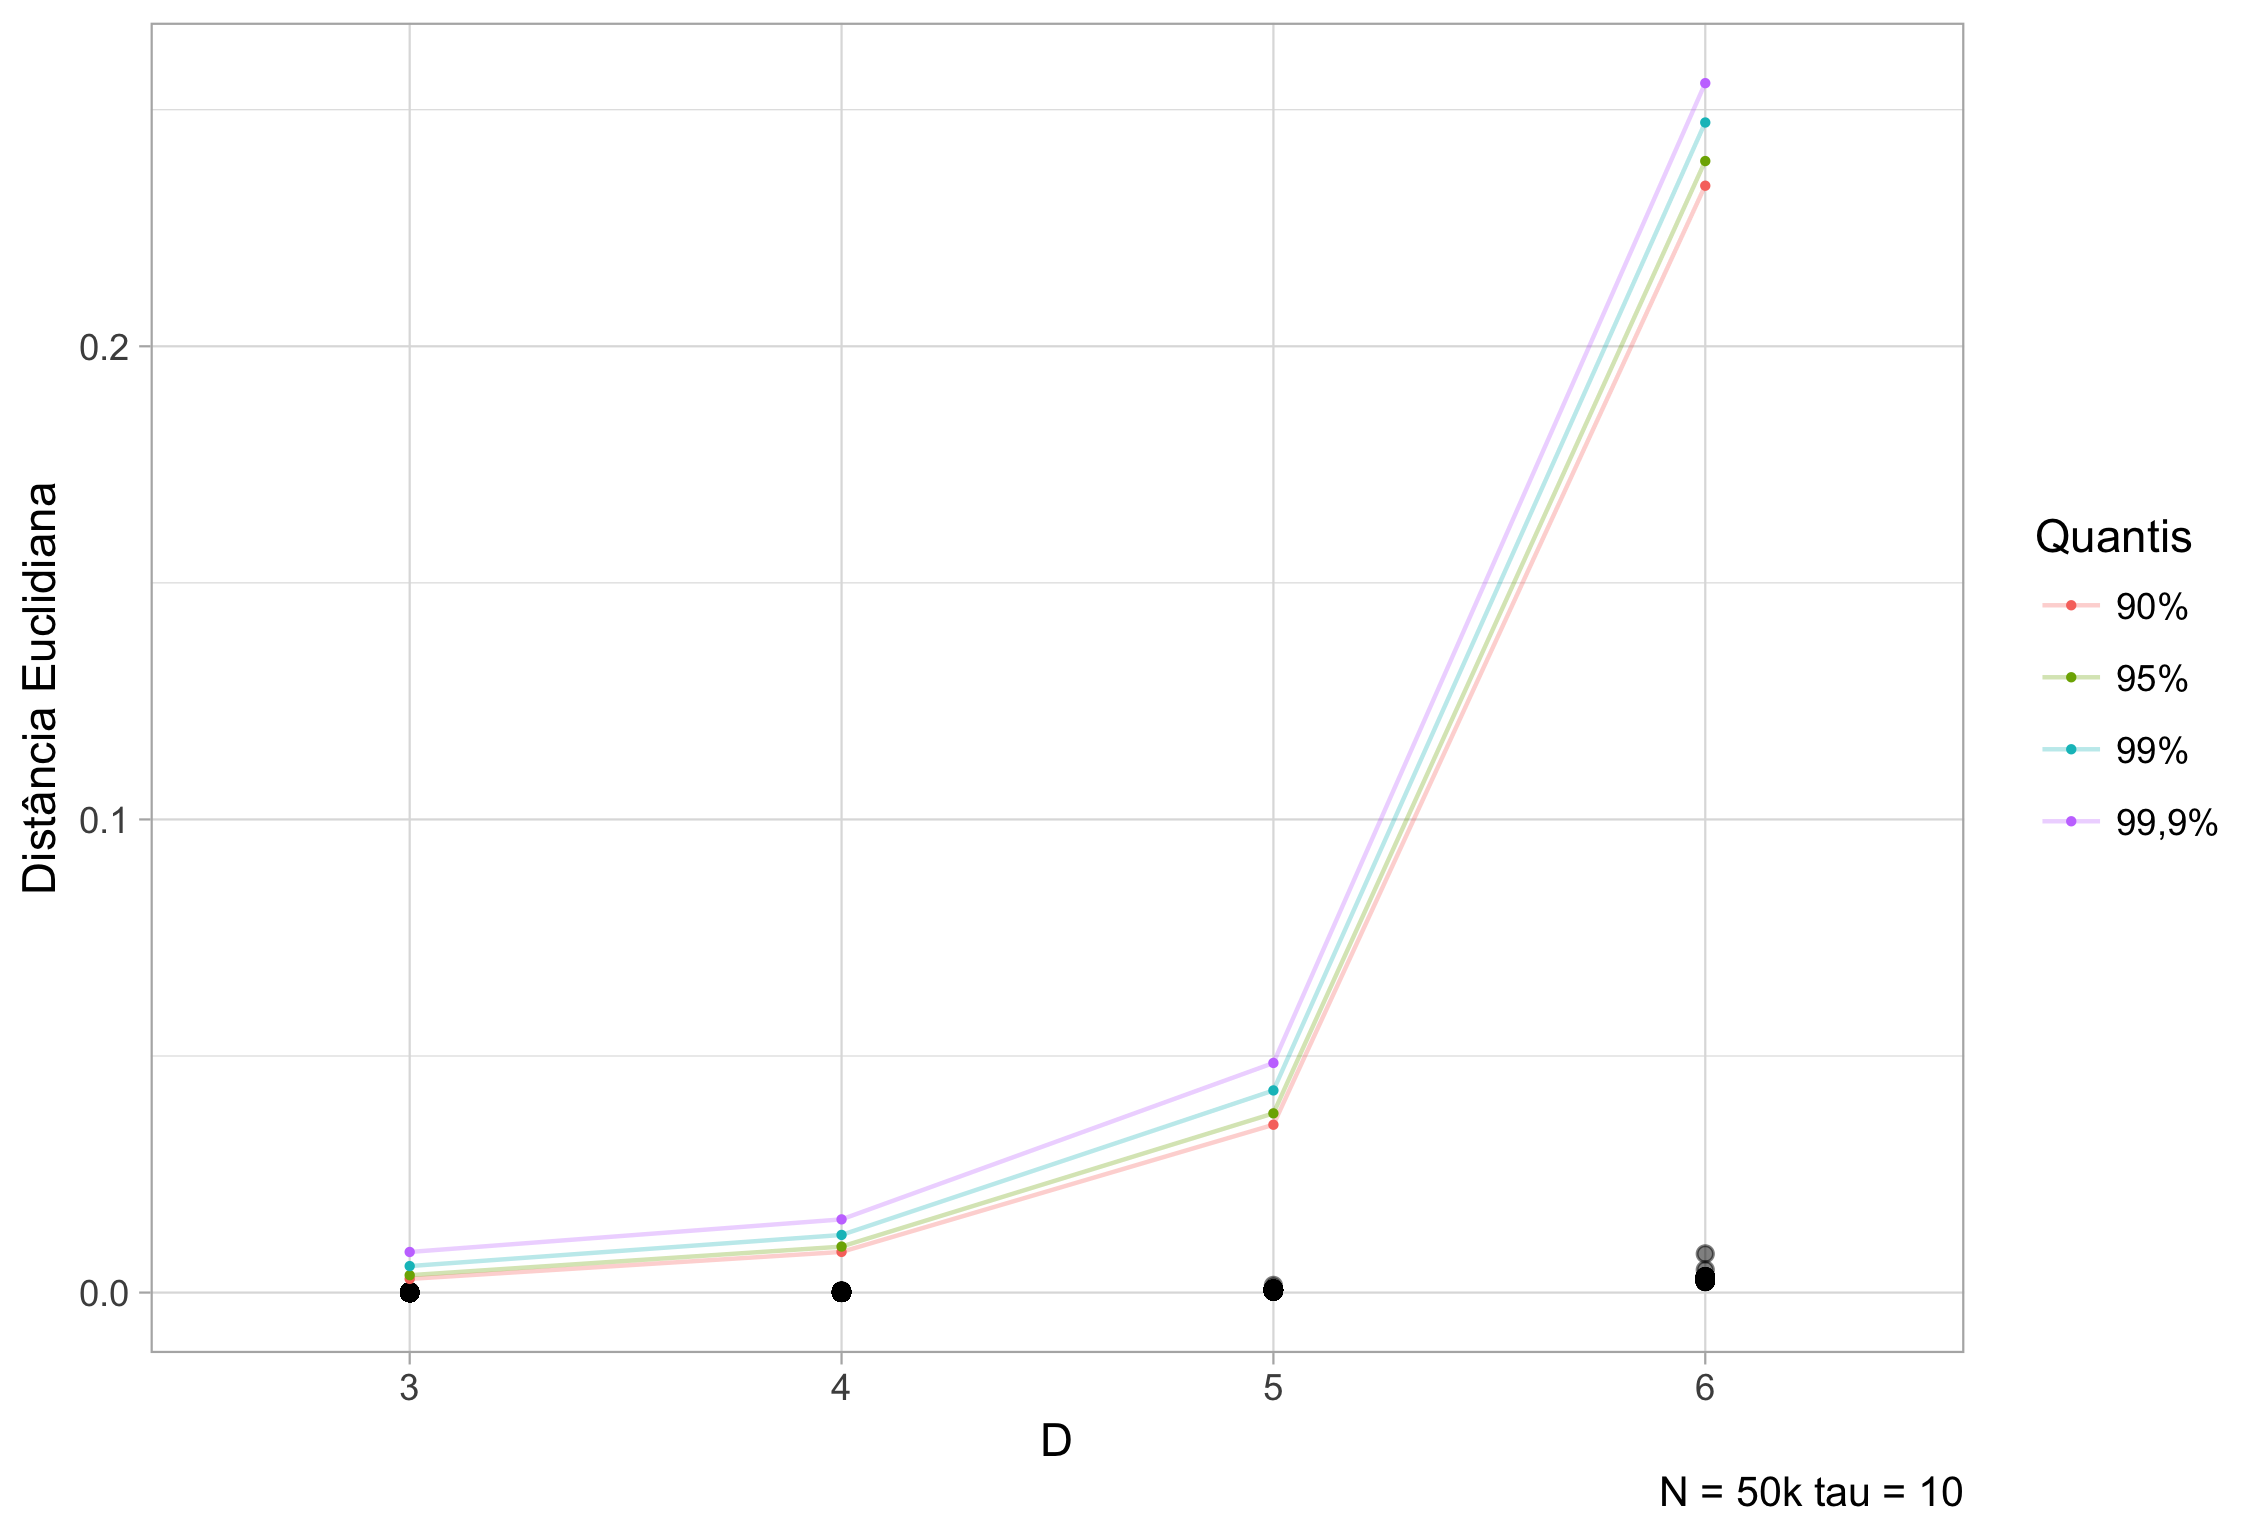
\includegraphics[width=.7\linewidth]{Conf_Int_50k_T10_noMT}
		\caption{Intervalos de confiança para o caso $N=50.000$ e $\tau=10$.}\label{Fig:Conf_Int_50k_T10}
		\end{figure}
		
	\end{block}
\end{frame}

\begin{frame}{Resultados}{Análise das regiões de confiança}
	\begin{block}{$N=50.000$ e $\tau=30$}
	\begin{figure}
		\centering
		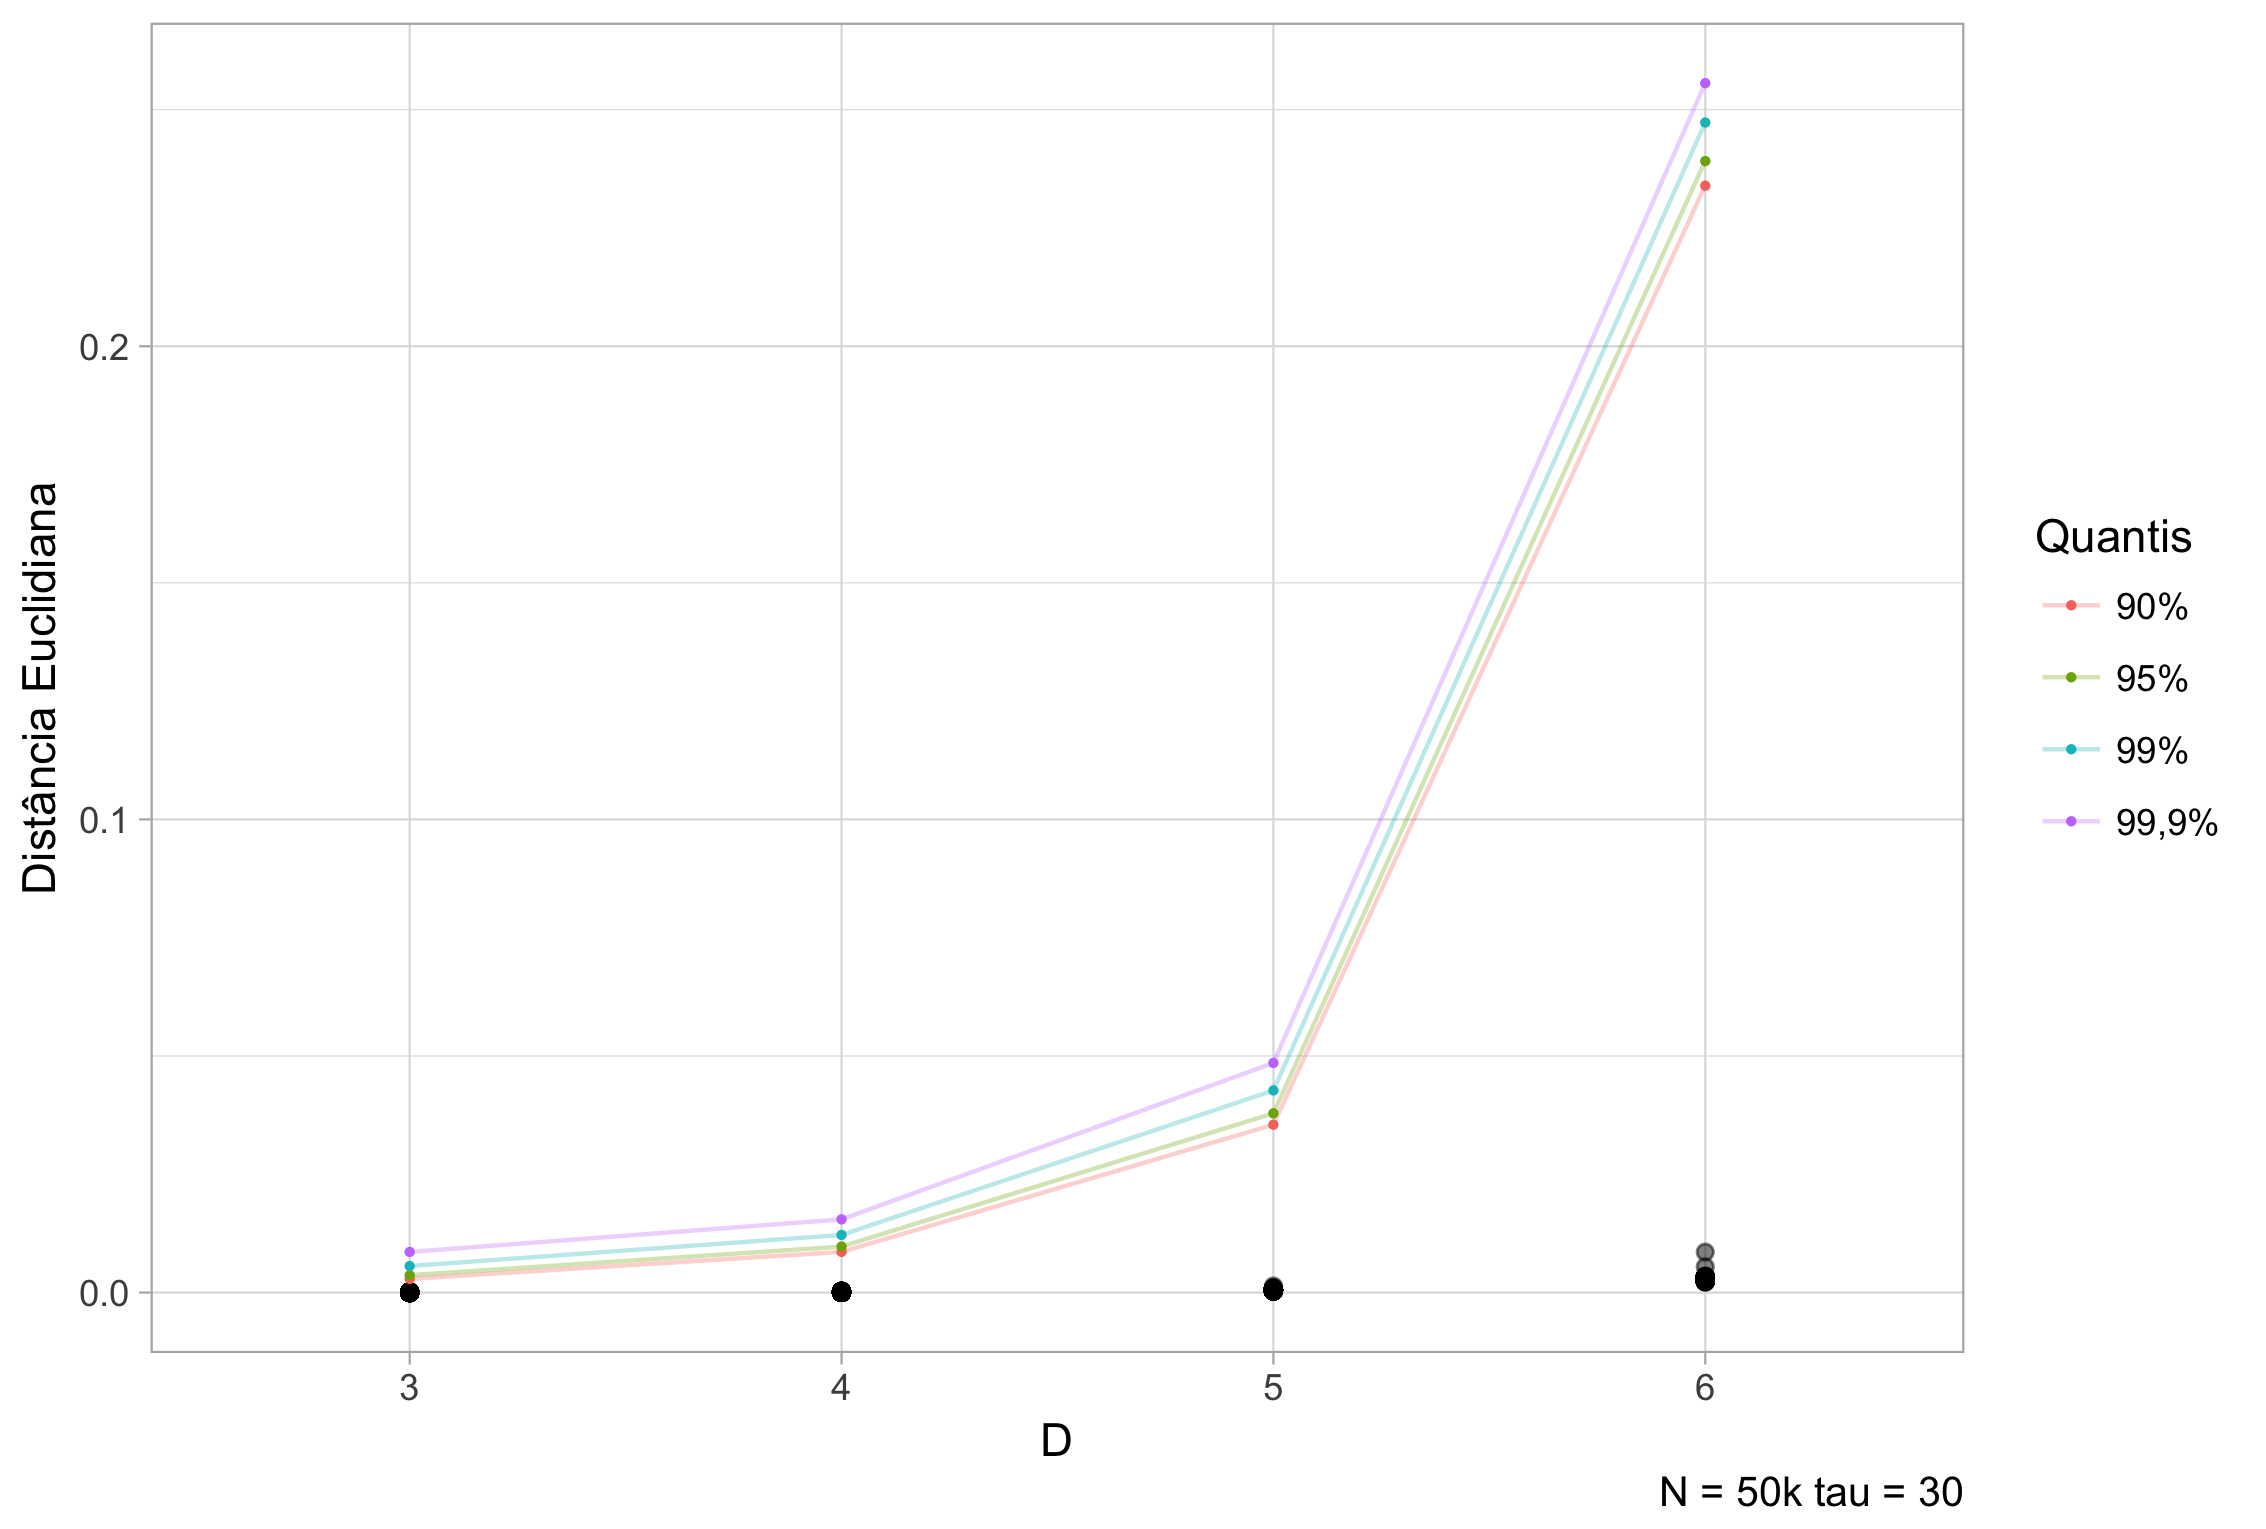
\includegraphics[width=.7\linewidth]{Conf_Int_50k_T30_noMT}
		\caption{Intervalos de confiança para o caso $N=50.000$ e $\tau=30$.}\label{Fig:Conf_Int_50k_30}
	\end{figure}
	\end{block}
\end{frame}

\begin{frame}{Resultados}{Análise das regiões de confiança}
	\begin{block}{$N=50.000$ e $\tau=50$}
	\begin{figure}
		\centering
		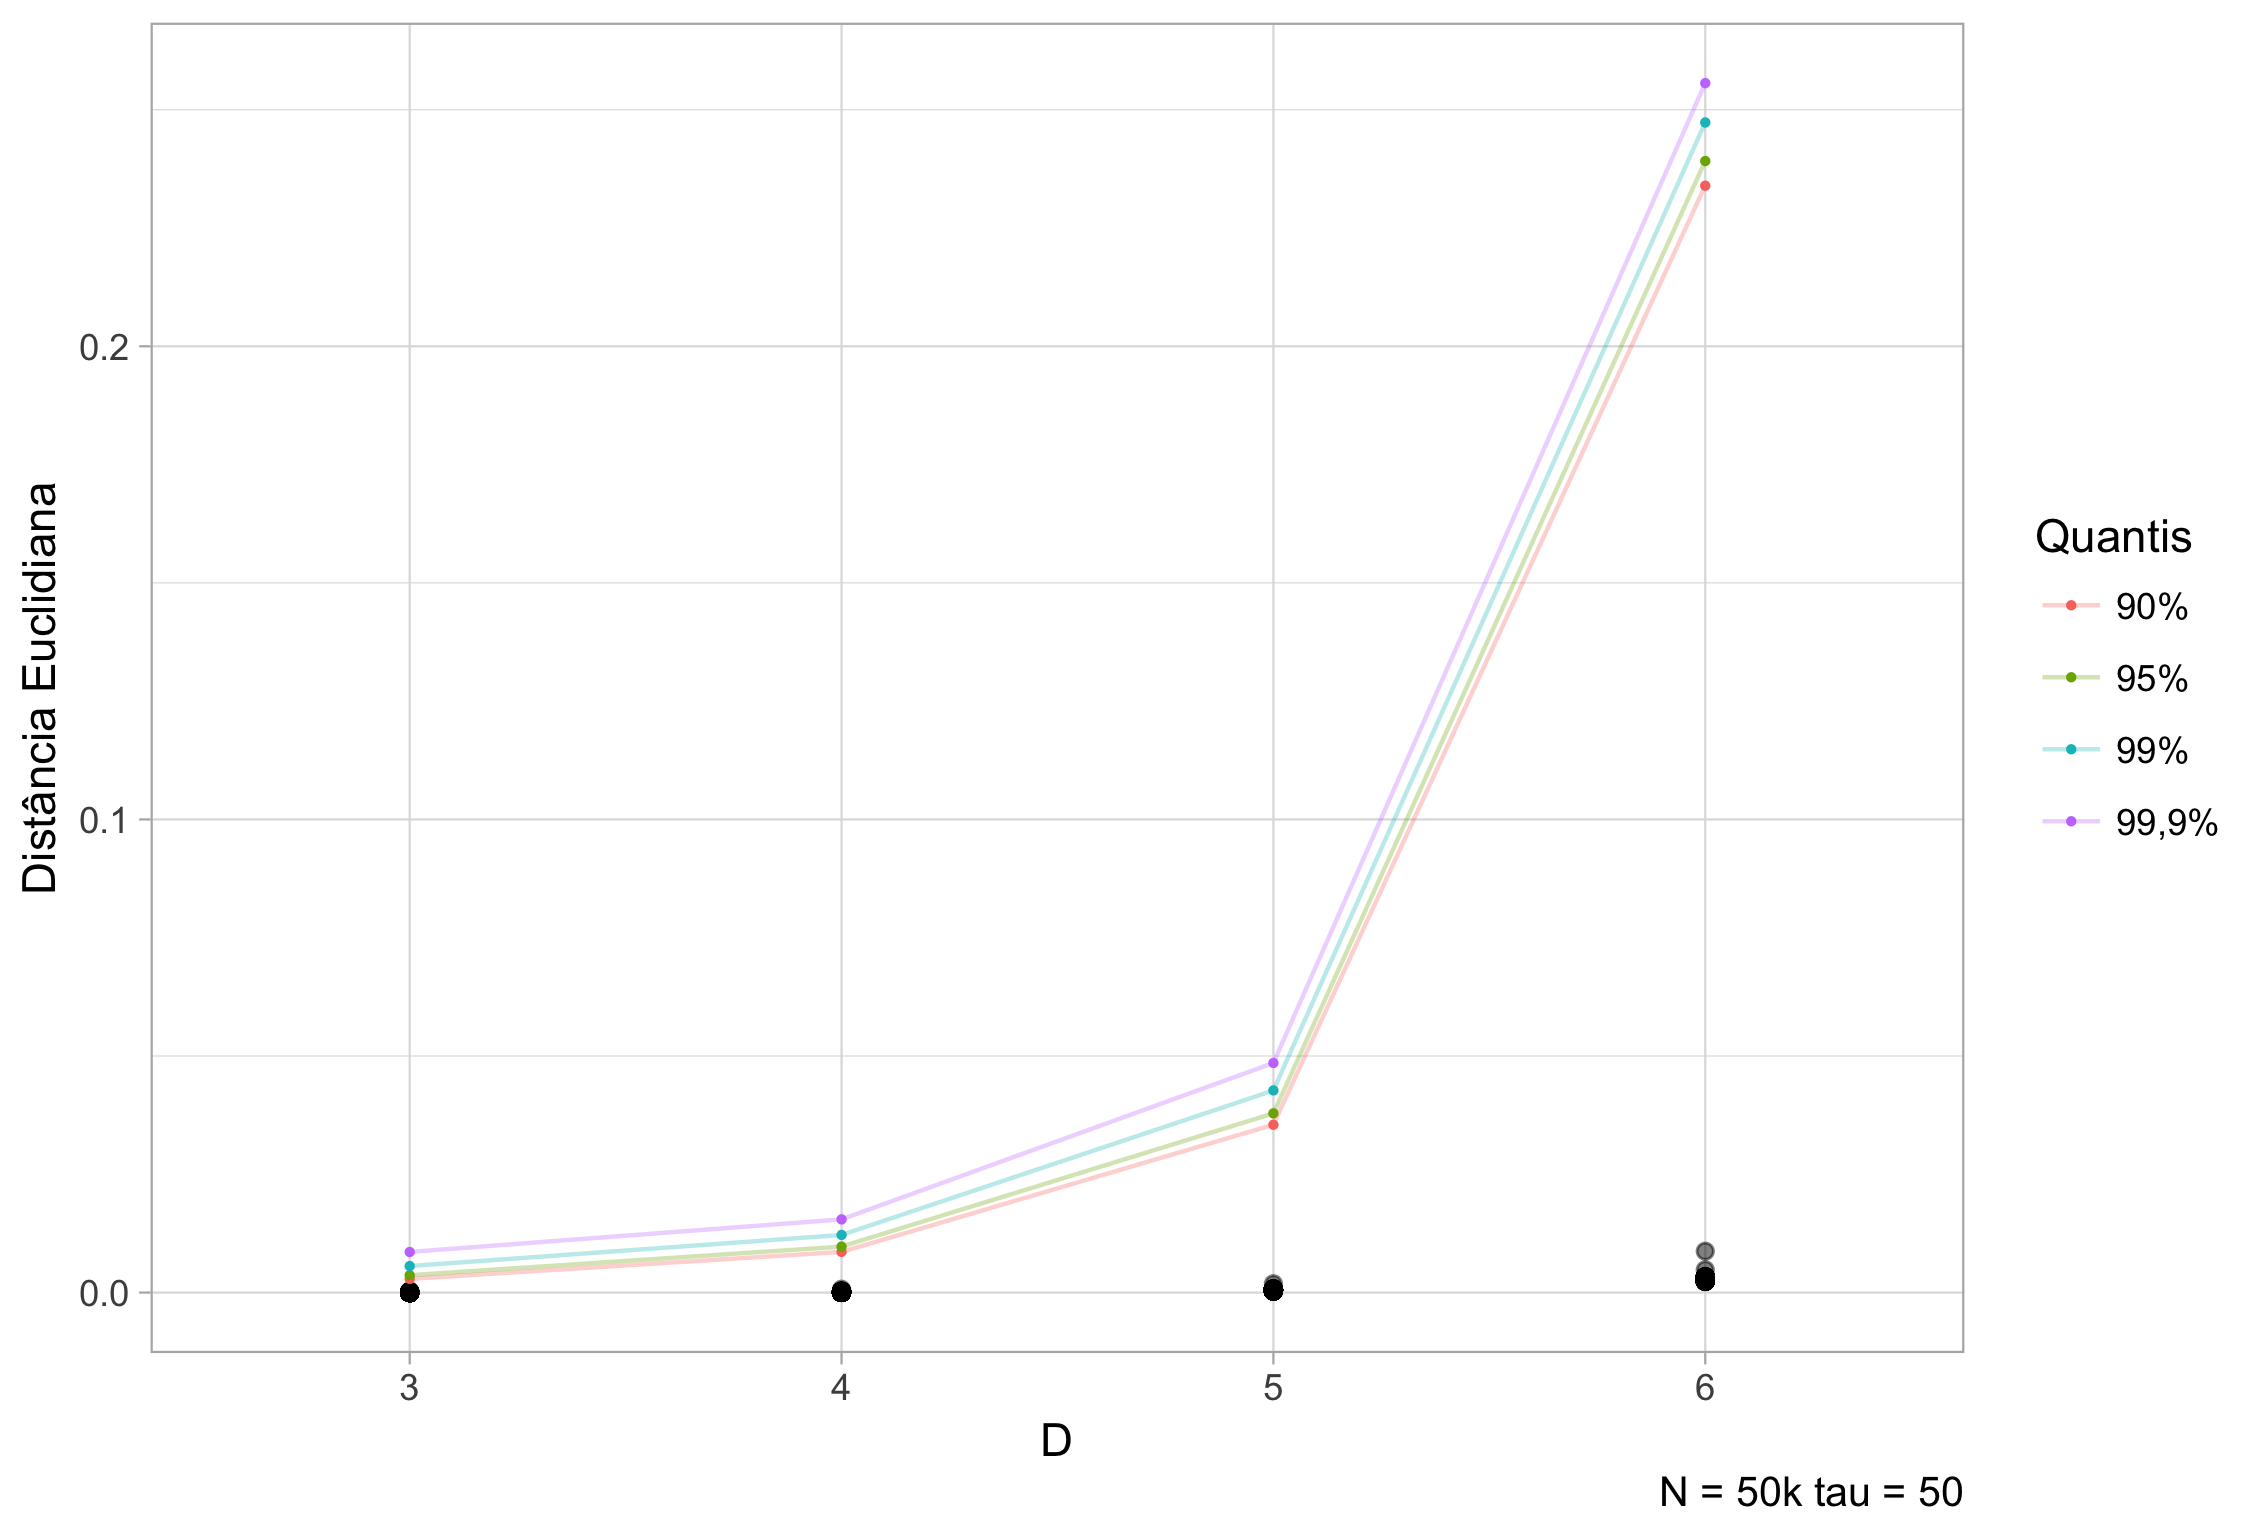
\includegraphics[width=.7\linewidth]{Conf_Int_50k_T50_noMT}
		\caption{Intervalos de confiança para o caso $N=50.000$ e $\tau=50$.}\label{Fig:Conf_Int_50k_T50}
	\end{figure}	
	\end{block}
\end{frame}

\begin{frame}{Resultados}{}
	\begin{block}{Quantis das distâncias, sequências de $50.000$ observações.}
	\resizebox{\linewidth}{!}{% Resize table to fit within \linewidth horizontally	
		\centering
		\begin{tabular}{ccccccc}
			\toprule
			$N = 50.000$	&  $D$  &$\tau$  &\SI{90}{\percent}&\SI{95}{\percent}&\SI{99}{\percent}&\SI{99.9}{\percent}\\ 
			\midrule
			&  $3$  &  $ 1$  &  5.407679e-05  &  7.015910e-05  &  0.0001178519  &  0.0001917689 \\ 
			&  $3$  &  $10$  &  5.636160e-05  &  7.130762e-05  &  0.0001000853  &  0.0001585019 \\
			&  $3$  &  $30$  &  5.731458e-05  &  7.245769e-05  &  0.0001101931  &  0.0001580179 \\
			&  $3$  &  $50$  &  5.951595e-05  &  7.541980e-05  &  0.0001093136  &  0.0001983728 \\ 
			\midrule
			&  $4$  &  $ 1$  &  1.589081e-04  &  1.818144e-04  &  0.0002250318  &  0.0003038889 \\ 
			&  $4$  &  $10$  &  1.588585e-04  &  1.790301e-04  &  0.0002264259  &  0.0002903681 \\
			&  $4$  &  $30$  &  1.631504e-04  &  1.863802e-04  &  0.0002330694  &  0.0002893557 \\
			&  $4$  &  $50$  &  1.619028e-04  &  1.809200e-04  &  0.0002311957  &  0.0003017229 \\ 
			\midrule
			&  $5$  &  $ 1$  &  6.062508e-04  &  6.389830e-04  &  0.0007179730  &  0.0008832568 \\ 
			&  $5$  &  $10$  &  5.985032e-04  &  6.289105e-04  &  0.0007041024  &  0.0007855387 \\
			&  $5$  &  $30$  &  6.040569e-04  &  6.400727e-04  &  0.0007268196  &  0.0008213228 \\
			&  $5$  &  $50$  &  6.055769e-04  &  6.381391e-04  &  0.0007134216  &  0.0008042788 \\ 
			\midrule
			&  $6$  &  $ 1$  &  3.071590e-03  &  3.150152e-03  &  0.0033104814  &  0.0035923810 \\ 
			&  $6$  &  $10$  &  3.050841e-03  &  3.117779e-03  &  0.0032553996  &  0.0033734229 \\
			&  $6$  &  $30$  &  3.066360e-03  &  3.129649e-03  &  0.0032669327  &  0.0034581195 \\
			&  $6$  &  $50$  &  3.074748e-03  &  3.147889e-03  &  0.0032828968  &  0.0034178859 \\
%			\bottomrule		
		\end{tabular}}
		\end{block}
	\end{frame}

%-------------------------------------------------------
\subsection{Aplicações}
%-------------------------------------------------------
\begin{frame}{Resultados}{Aplicações}
	\begin{block}{Aplicações}
		Nesta seção mostramos a aplicação da nossa proposta a sequências de tamanho \num{1000}.
		
		Utilizando a metodologia descrita, aplicamos o teste a uma seqência de \num{1000} observações produzidas pelos geradores Mersenne-Twister e Randu, além de séries não estacionárias, estacionárias e mapas logísticos, todos com a mesma dimensão.
		
	\end{block}
\end{frame}

\begin{frame}{Resultados}{Aplicações}
	\begin{block}{Aplicações - Mersenne-Twister e Randu}
	\begin{figure}
		\centering
		\subfigure[Mersenne-Twister. \label{ConfidInt_MT_1k_t1}]{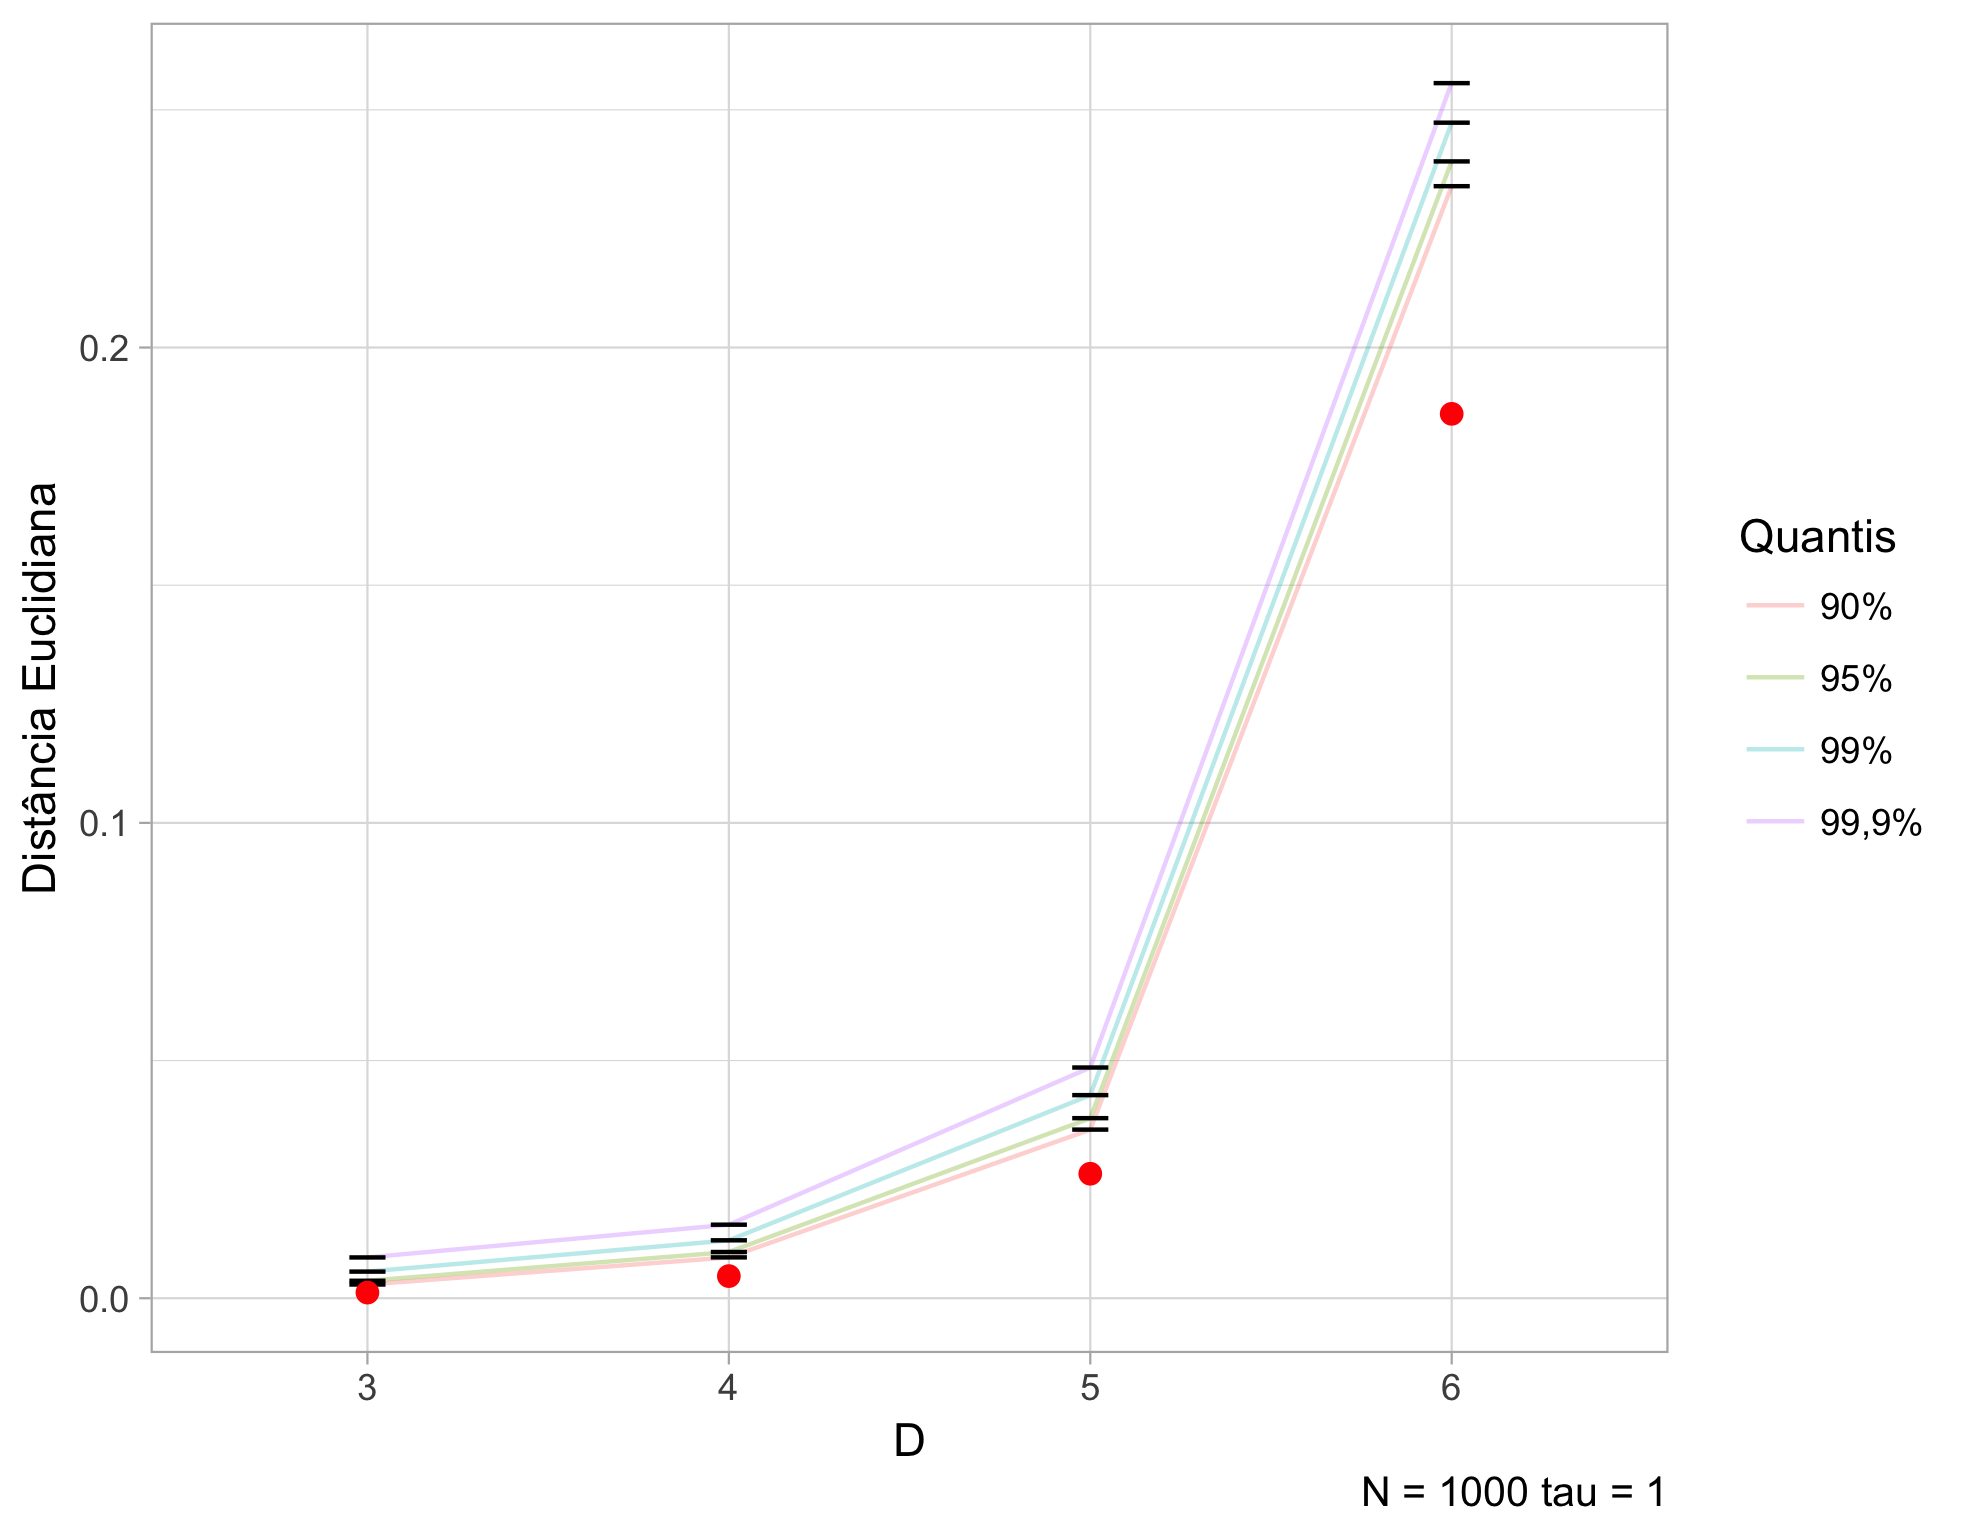
\includegraphics[width=.48\linewidth]{ConfidInt_MT_1k_t1}}
		\subfigure[Randu. \label{ConfidInt_Randu_1k_t1}]{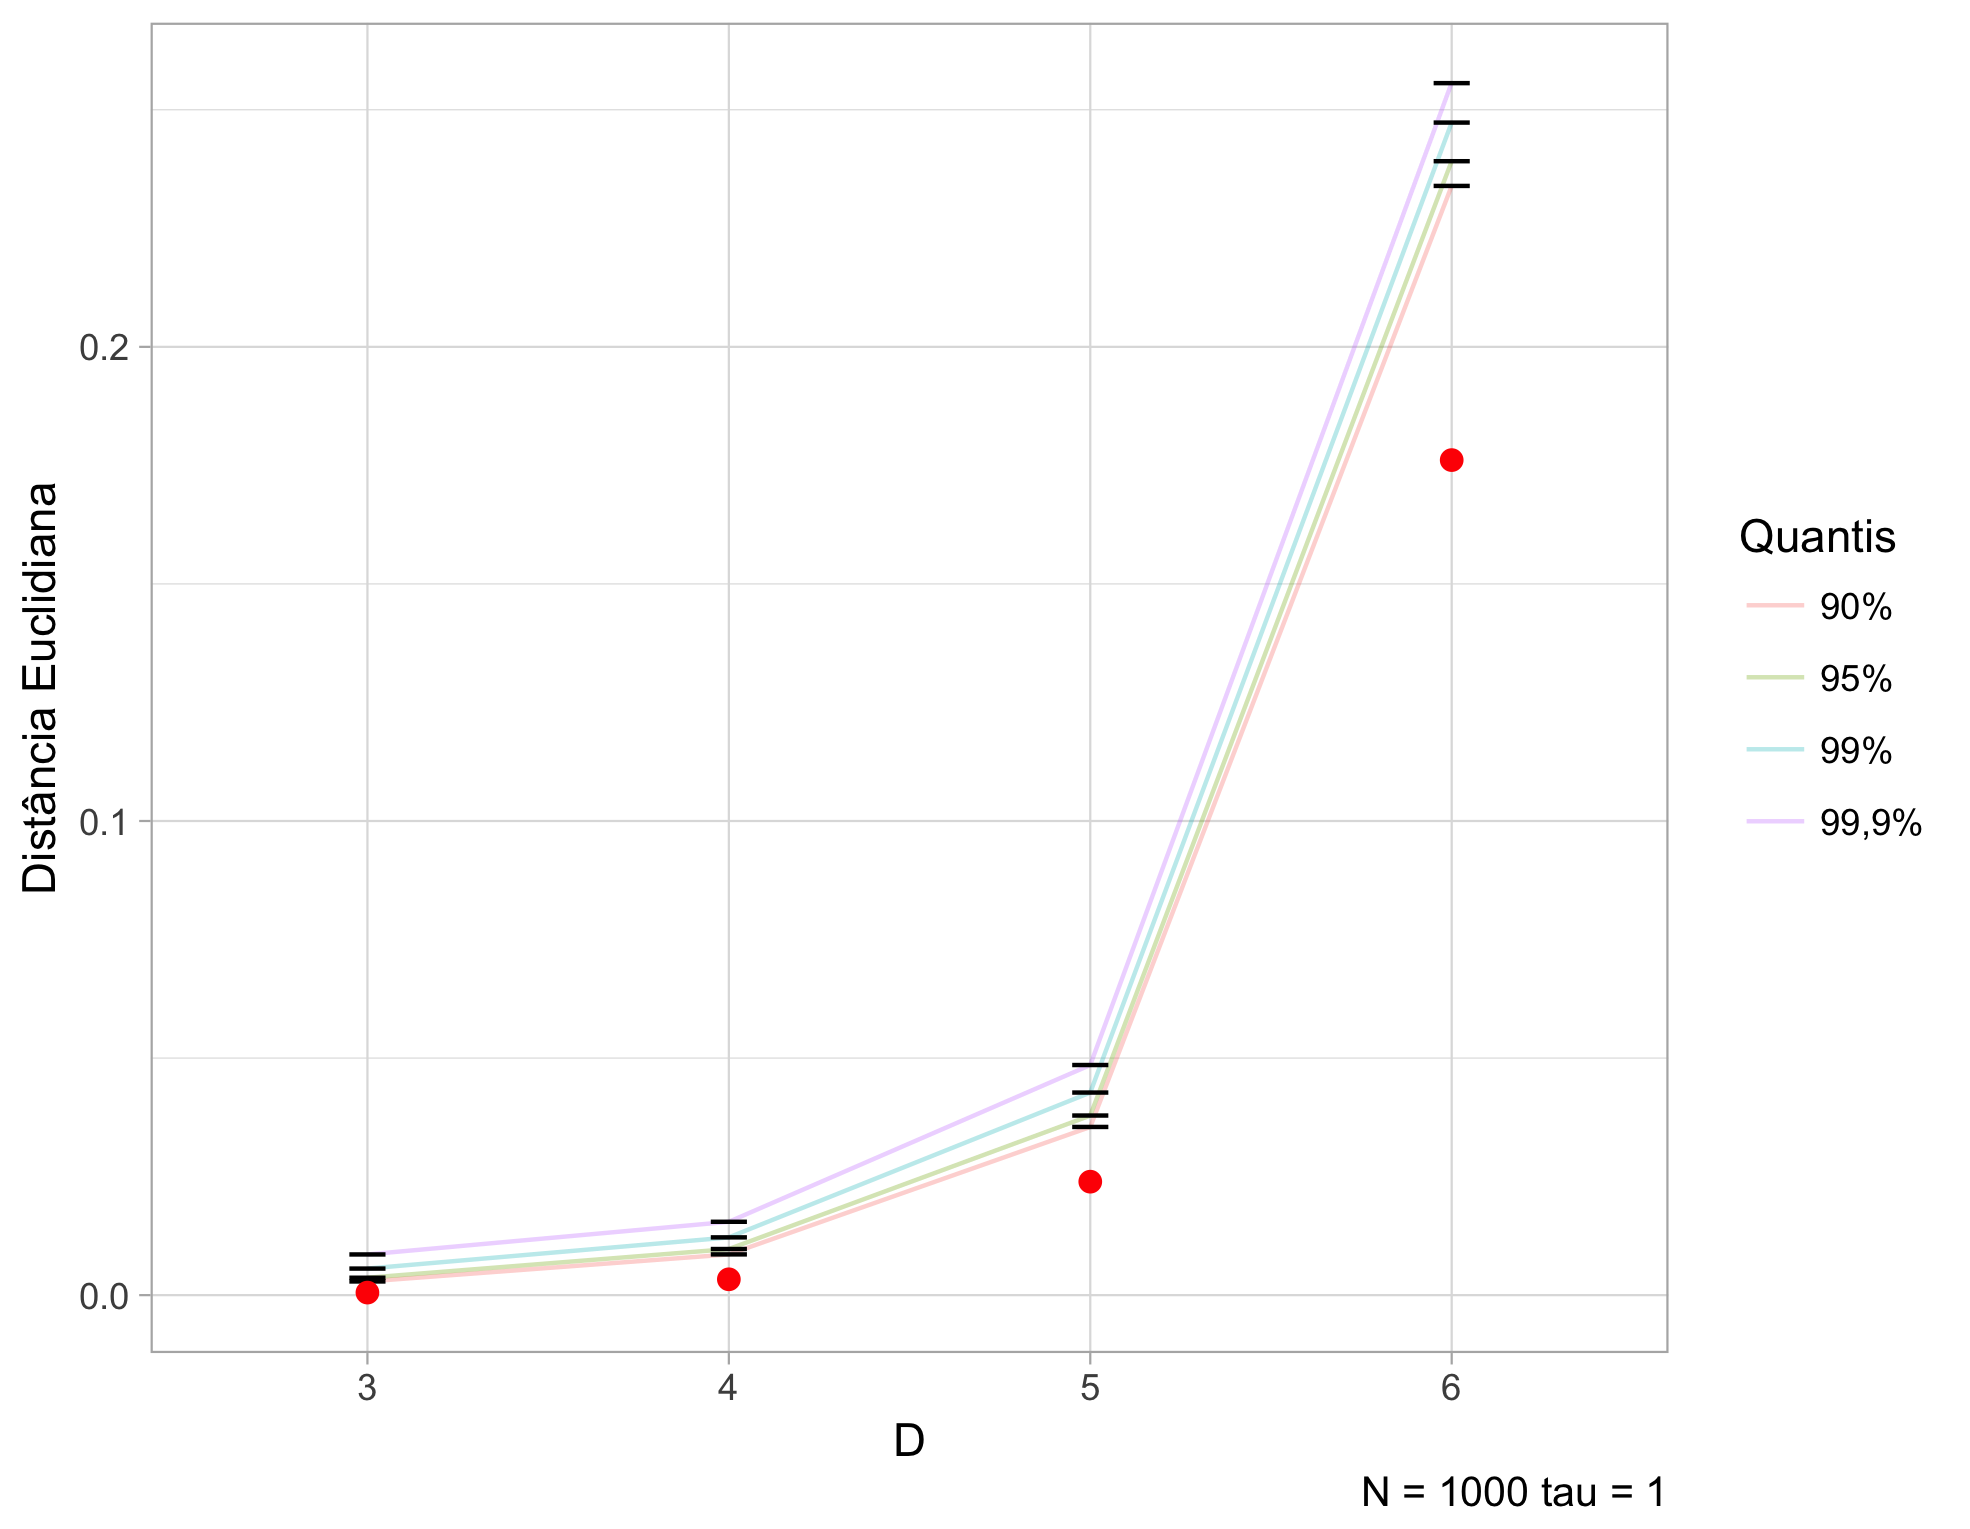
\includegraphics[width=.48\linewidth]{ConfidInt_Randu_1k_t1}}
		\caption{Aplicação do teste aos pontos de Mersenne-Twister e Randu}\label{fig:ConfInt_PRNGs}
	\end{figure}	
	\end{block}
\end{frame}

\begin{frame}{Resultados}{Aplicações}
	\begin{block}{Aplicações - Estruturas autocorrelacionadas}
	A seguir, geramos sequências estocásticas com estrutura de autocorrelação: uma estacionária (ruído gaussiano filtrado) e uma não estacionária (uma trajetória de movimento browniano).
	\end{block}
\end{frame}

\begin{frame}{Resultados}{Aplicações}
	\begin{block}{Aplicações - Séries não estacionárias}
		\begin{figure}
		\centering
		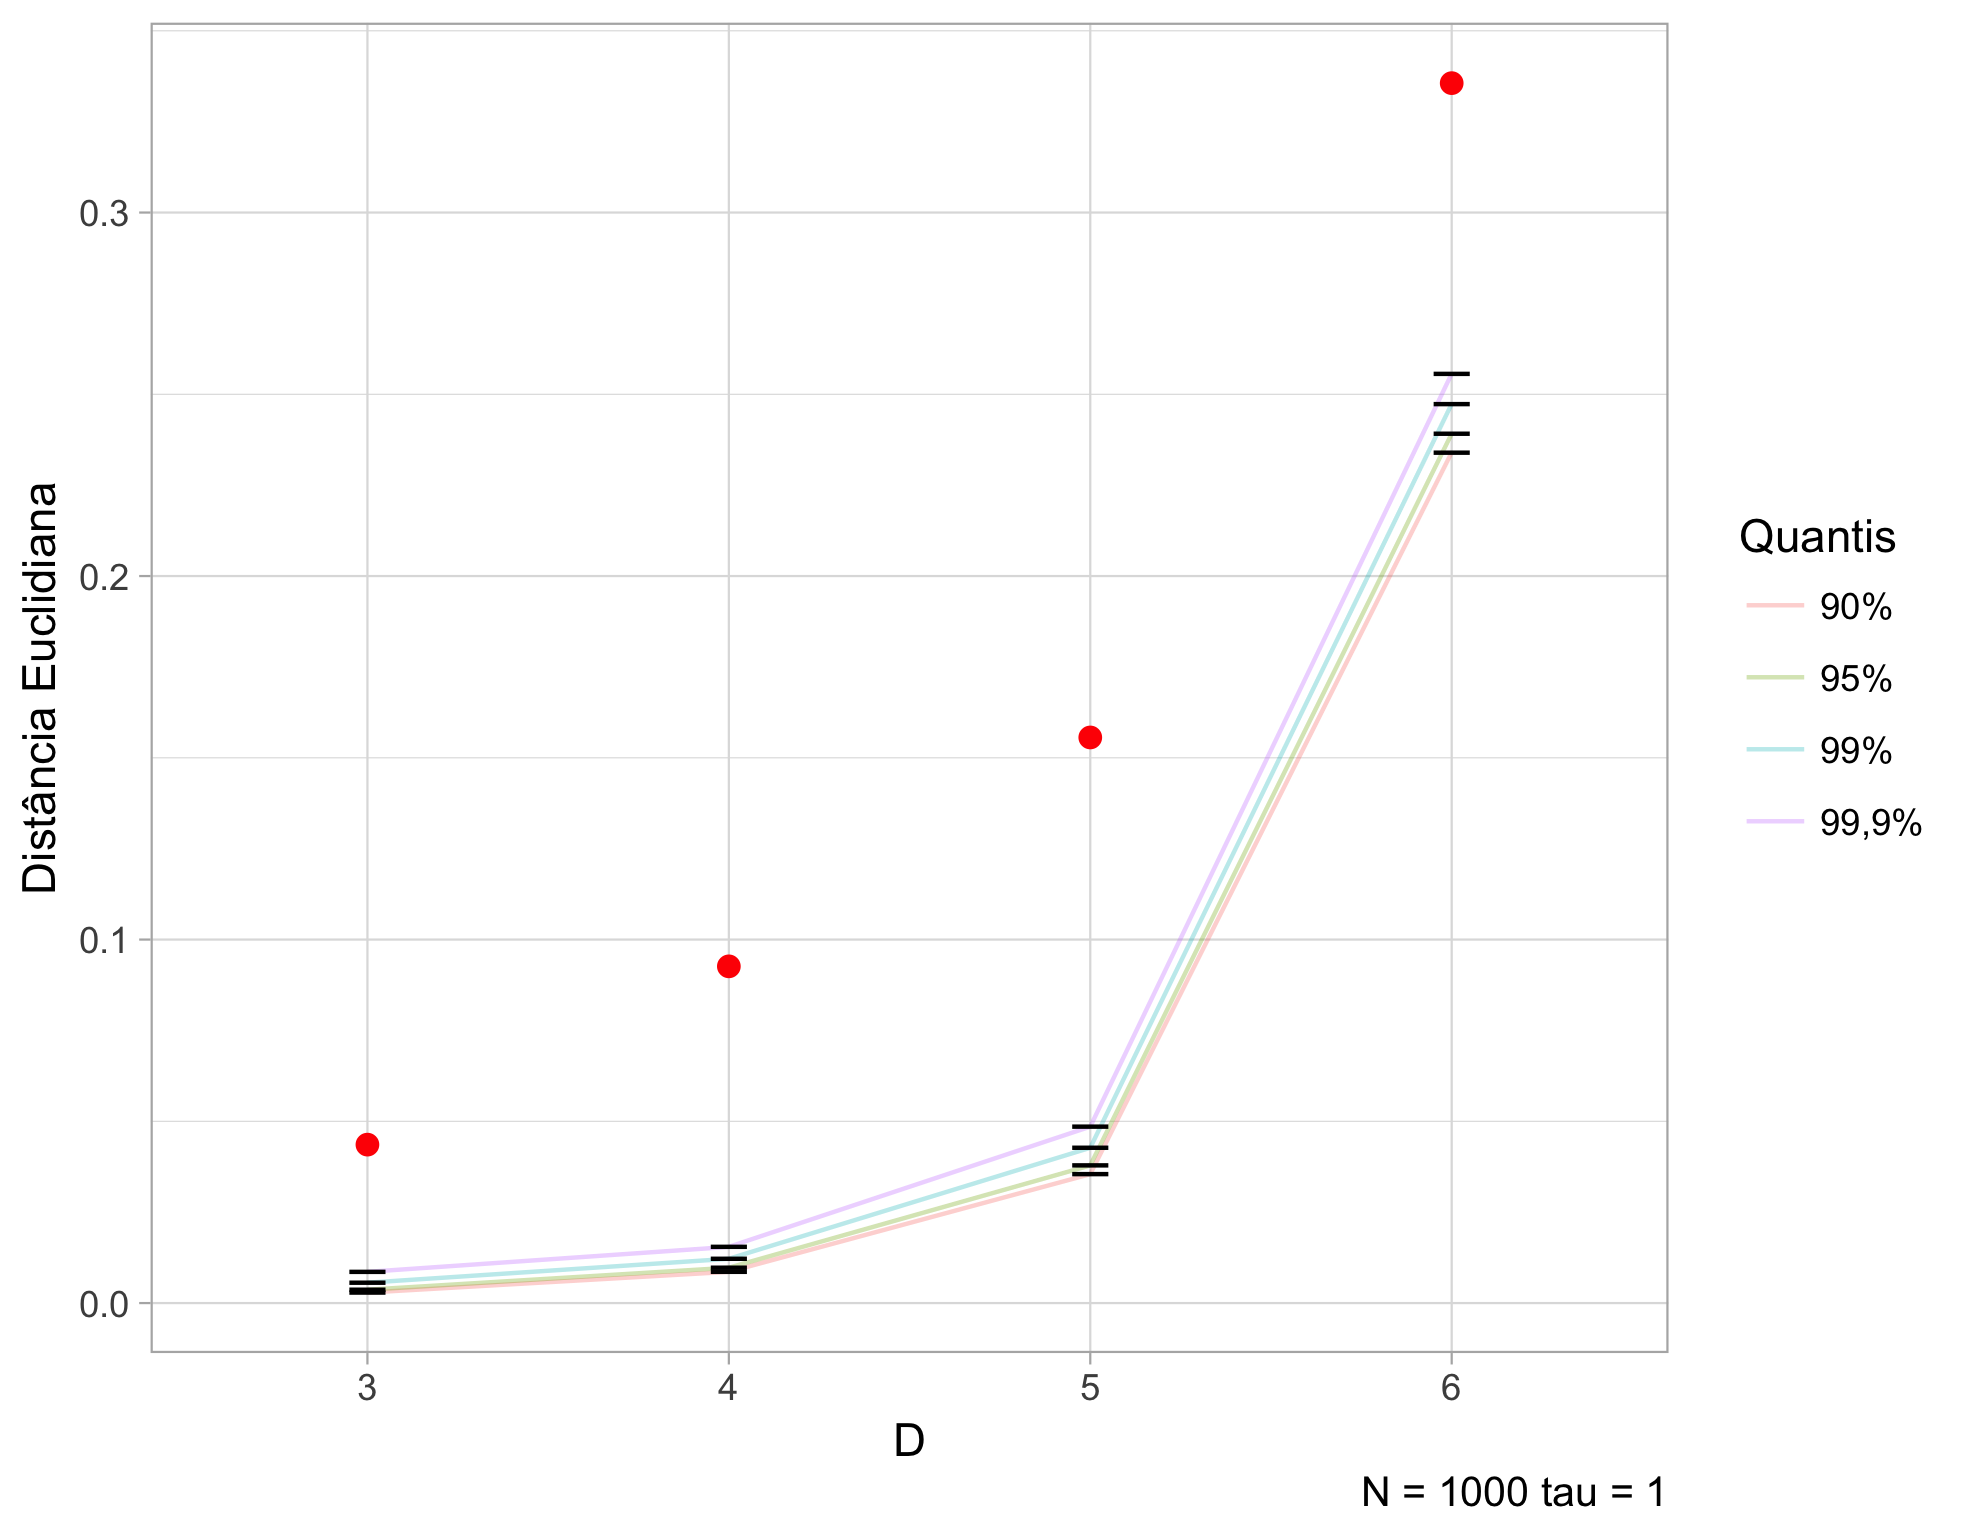
\includegraphics[width=.65\linewidth]{ConfidInt_nao_estacionaria_1k_t1}
		\caption{Pontos característicos das séries não estacionárias e intervalos de confiança.}\label{Fig:ConfidInt_nao_estacionaria_1k_t1}
		\end{figure}
	\end{block}
\end{frame}

\begin{frame}{Resultados}{Aplicações}
	\begin{block}{Aplicações - Série Estacionária}
	Uma série estacionária em que aplicamos nosso teste foi obtida pela convolução de uma sequência de variáveis aleatórias independentes e identicamente distribuídas segundo uma lei gaussiana padrão, convolucionada com uma máscara de tamanho \num{3} com valores não negativos: $(\beta,1,\beta)$, $0\leq \beta\leq 1$.
	\pause
	
	Quando $\beta$=\num{0} temos a sequência original, e para valores crescentes de $\beta$ temos sequências com cada vez maior estrutura de correlação.
	Calculamos o ponto característico da série assim obtida, e o contrastamos com os quantis empíricos obtidos anteriormente.	
	\end{block}
\end{frame}

\begin{frame}{Resultados}{Aplicações}
	\begin{block}{Aplicações - Poder do teste aplicado a Séries Estacionárias}
	\begin{figure}
		\centering
		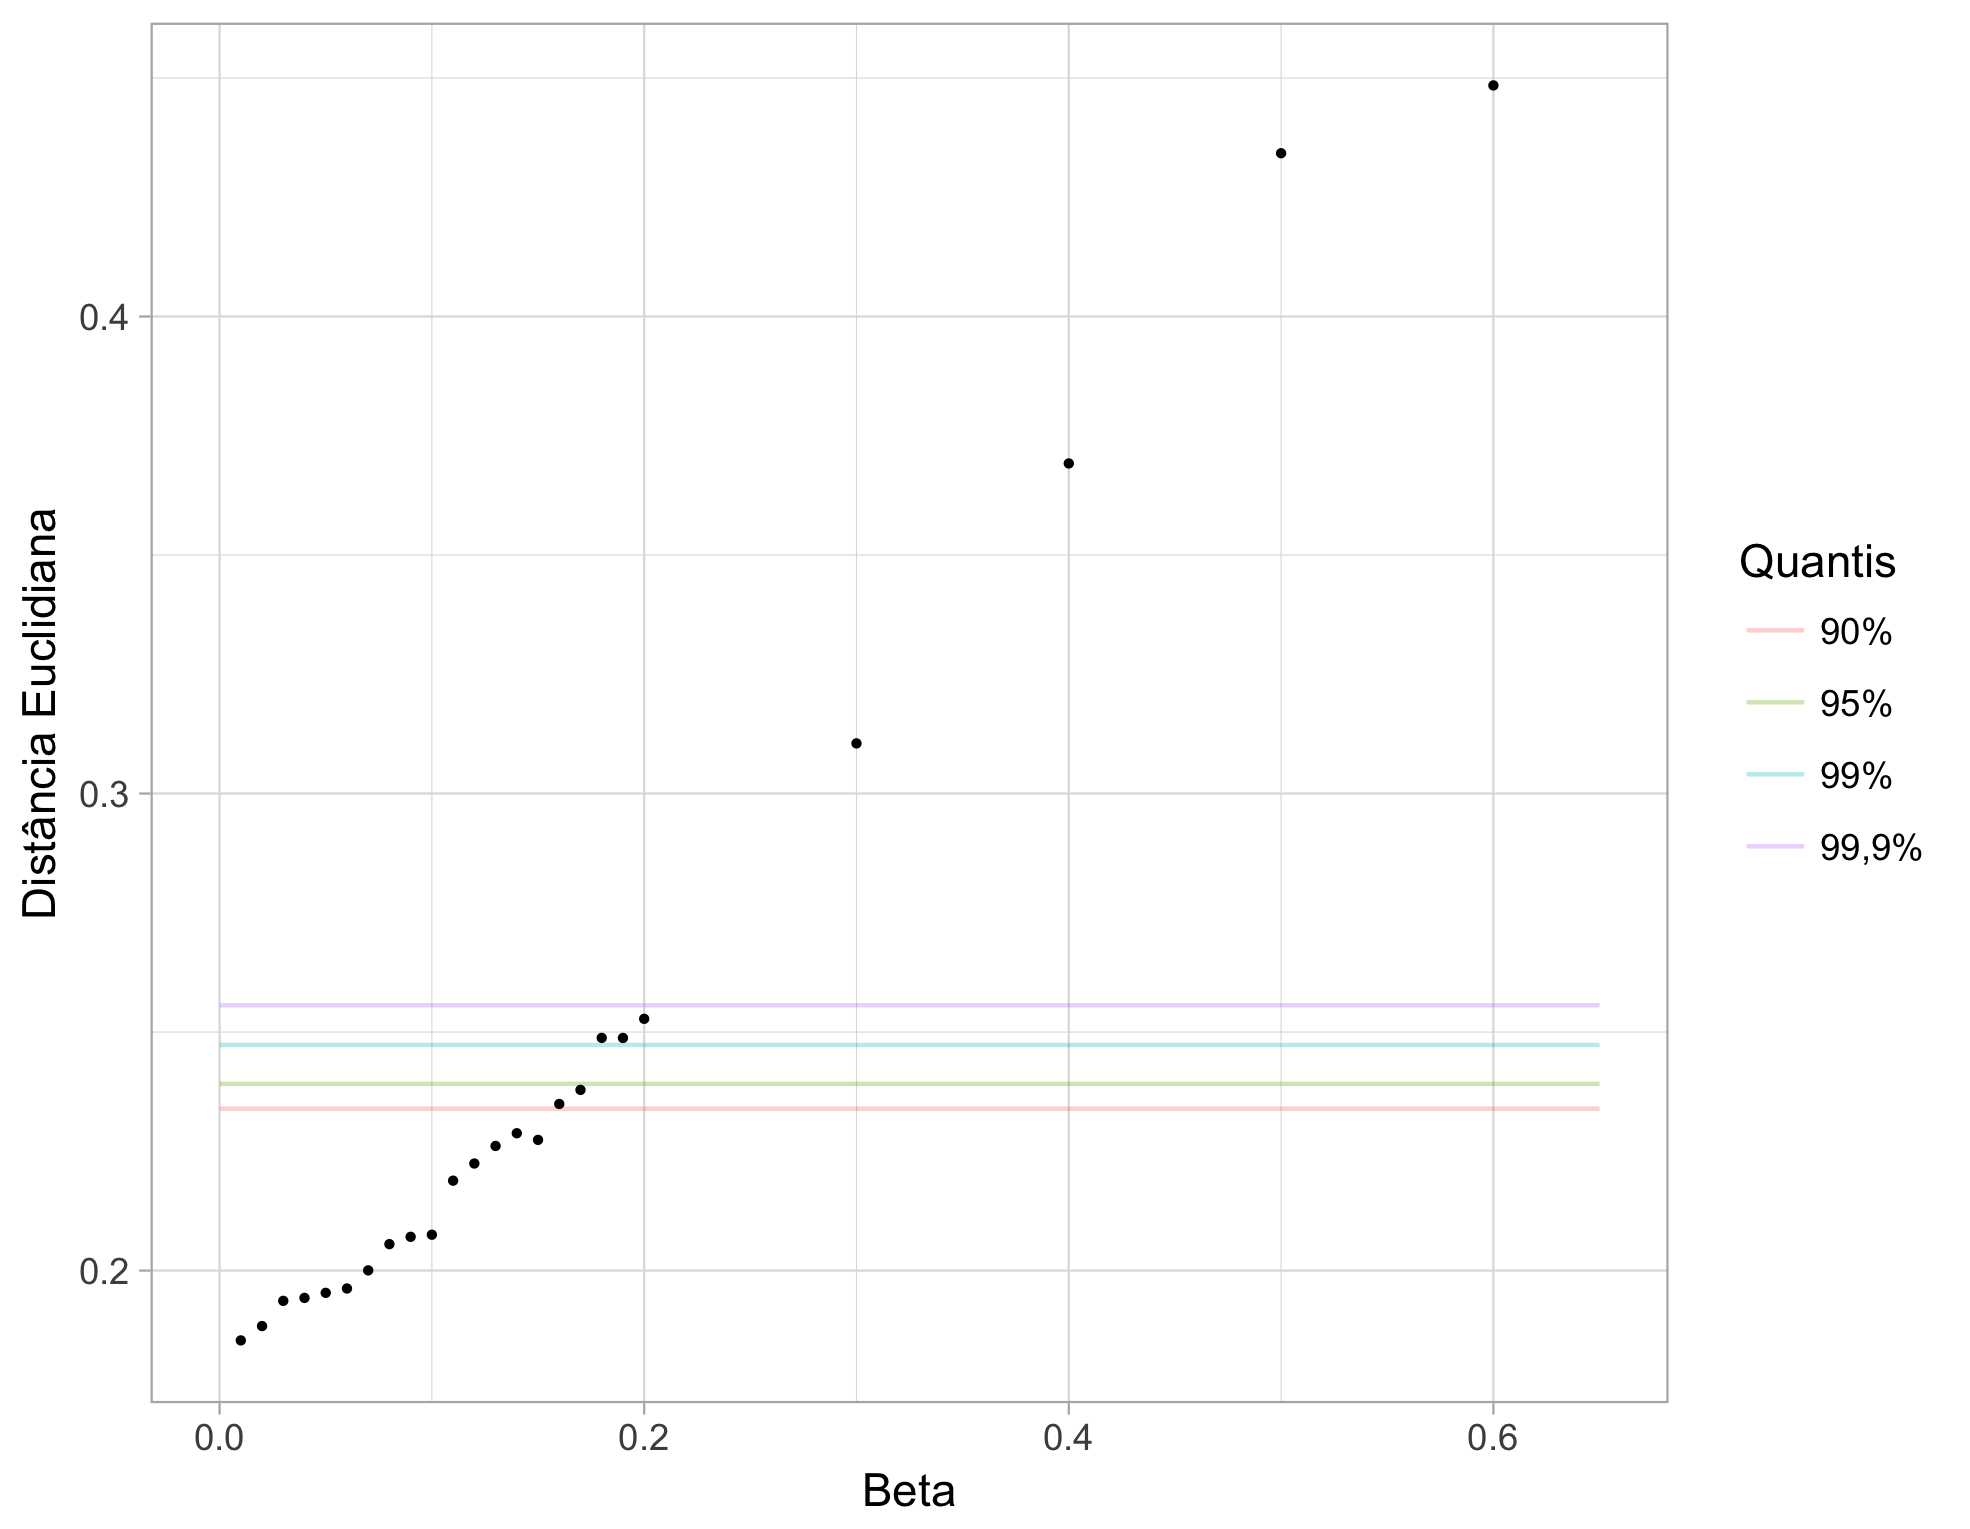
\includegraphics[width=.65\linewidth]{beta_1k_D6_t1}
		\caption{Poder do teste aplicado a uma sequência de séries estacionárias no caso particular $N=1.000$, $\tau=1$, variando-se a máscara de convolução $(\beta,1,\beta)$.}\label{Fig:beta}
	\end{figure}	
	\end{block}
\end{frame}

\begin{frame}{Resultados}{Aplicações}
	\begin{block}{Aplicações - Série Estacionária}
	\begin{figure}
		\centering
		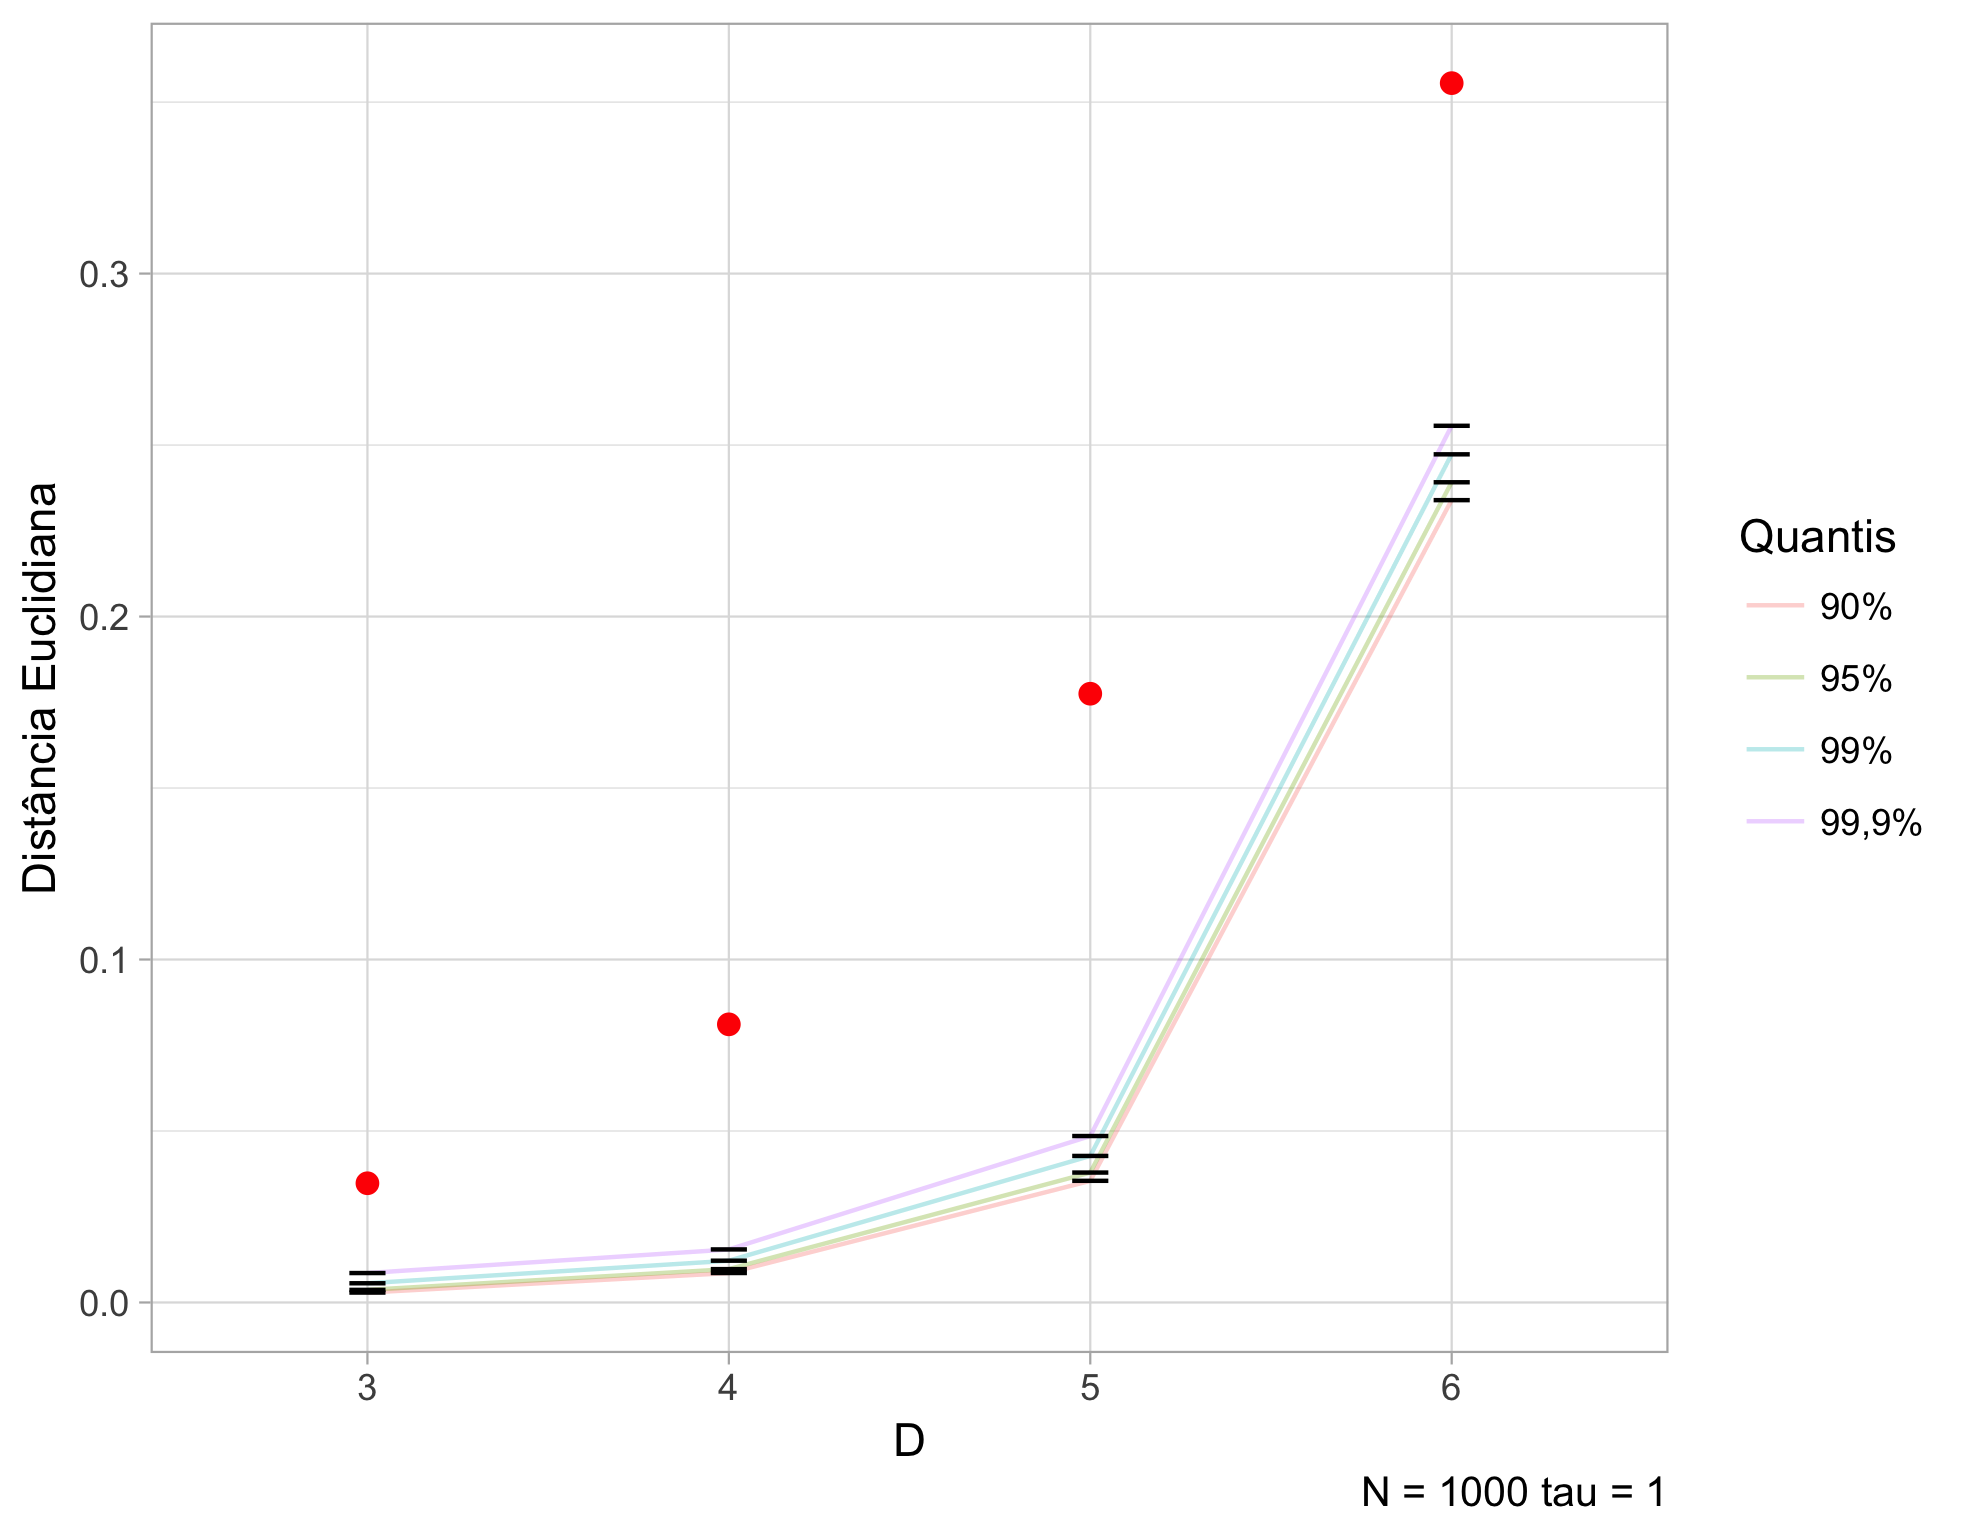
\includegraphics[width=.65\linewidth]{ConfidInt_estacionaria_1k_t1}
		\caption{Pontos característicos das séries estacionárias e intervalos de confiança.}\label{Fig:ConfidInt_estacionaria_1k_t1}
	\end{figure}	
	\end{block}
\end{frame}

\begin{frame}{Resultados}{Aplicações}
	\begin{block}{Aplicações - Mapa logístico}
	A seguir analisamos uma série determinística com comportamento caótico: o mapa logístico.
	O mapa logístico é a sequência obtida pela recursão
	\begin{equation}
	x_{n+1} = r x_n(1-x_n),
	\end{equation}
	com $0<x_1<1$ e $0<r\leq 4$.
	Utilizamos $r=4$, $x_0=0.01$.\\
	Iteramos o mapa \num{10000} vezes para alcançar estabilidade, e só coletamos a partir de $n=10001$.	
	\end{block}
\end{frame}

\begin{frame}{Resultados}{Aplicações}
	\begin{block}{Aplicações - Mersenne-Twister e Randu}
	\begin{figure}
		\centering
		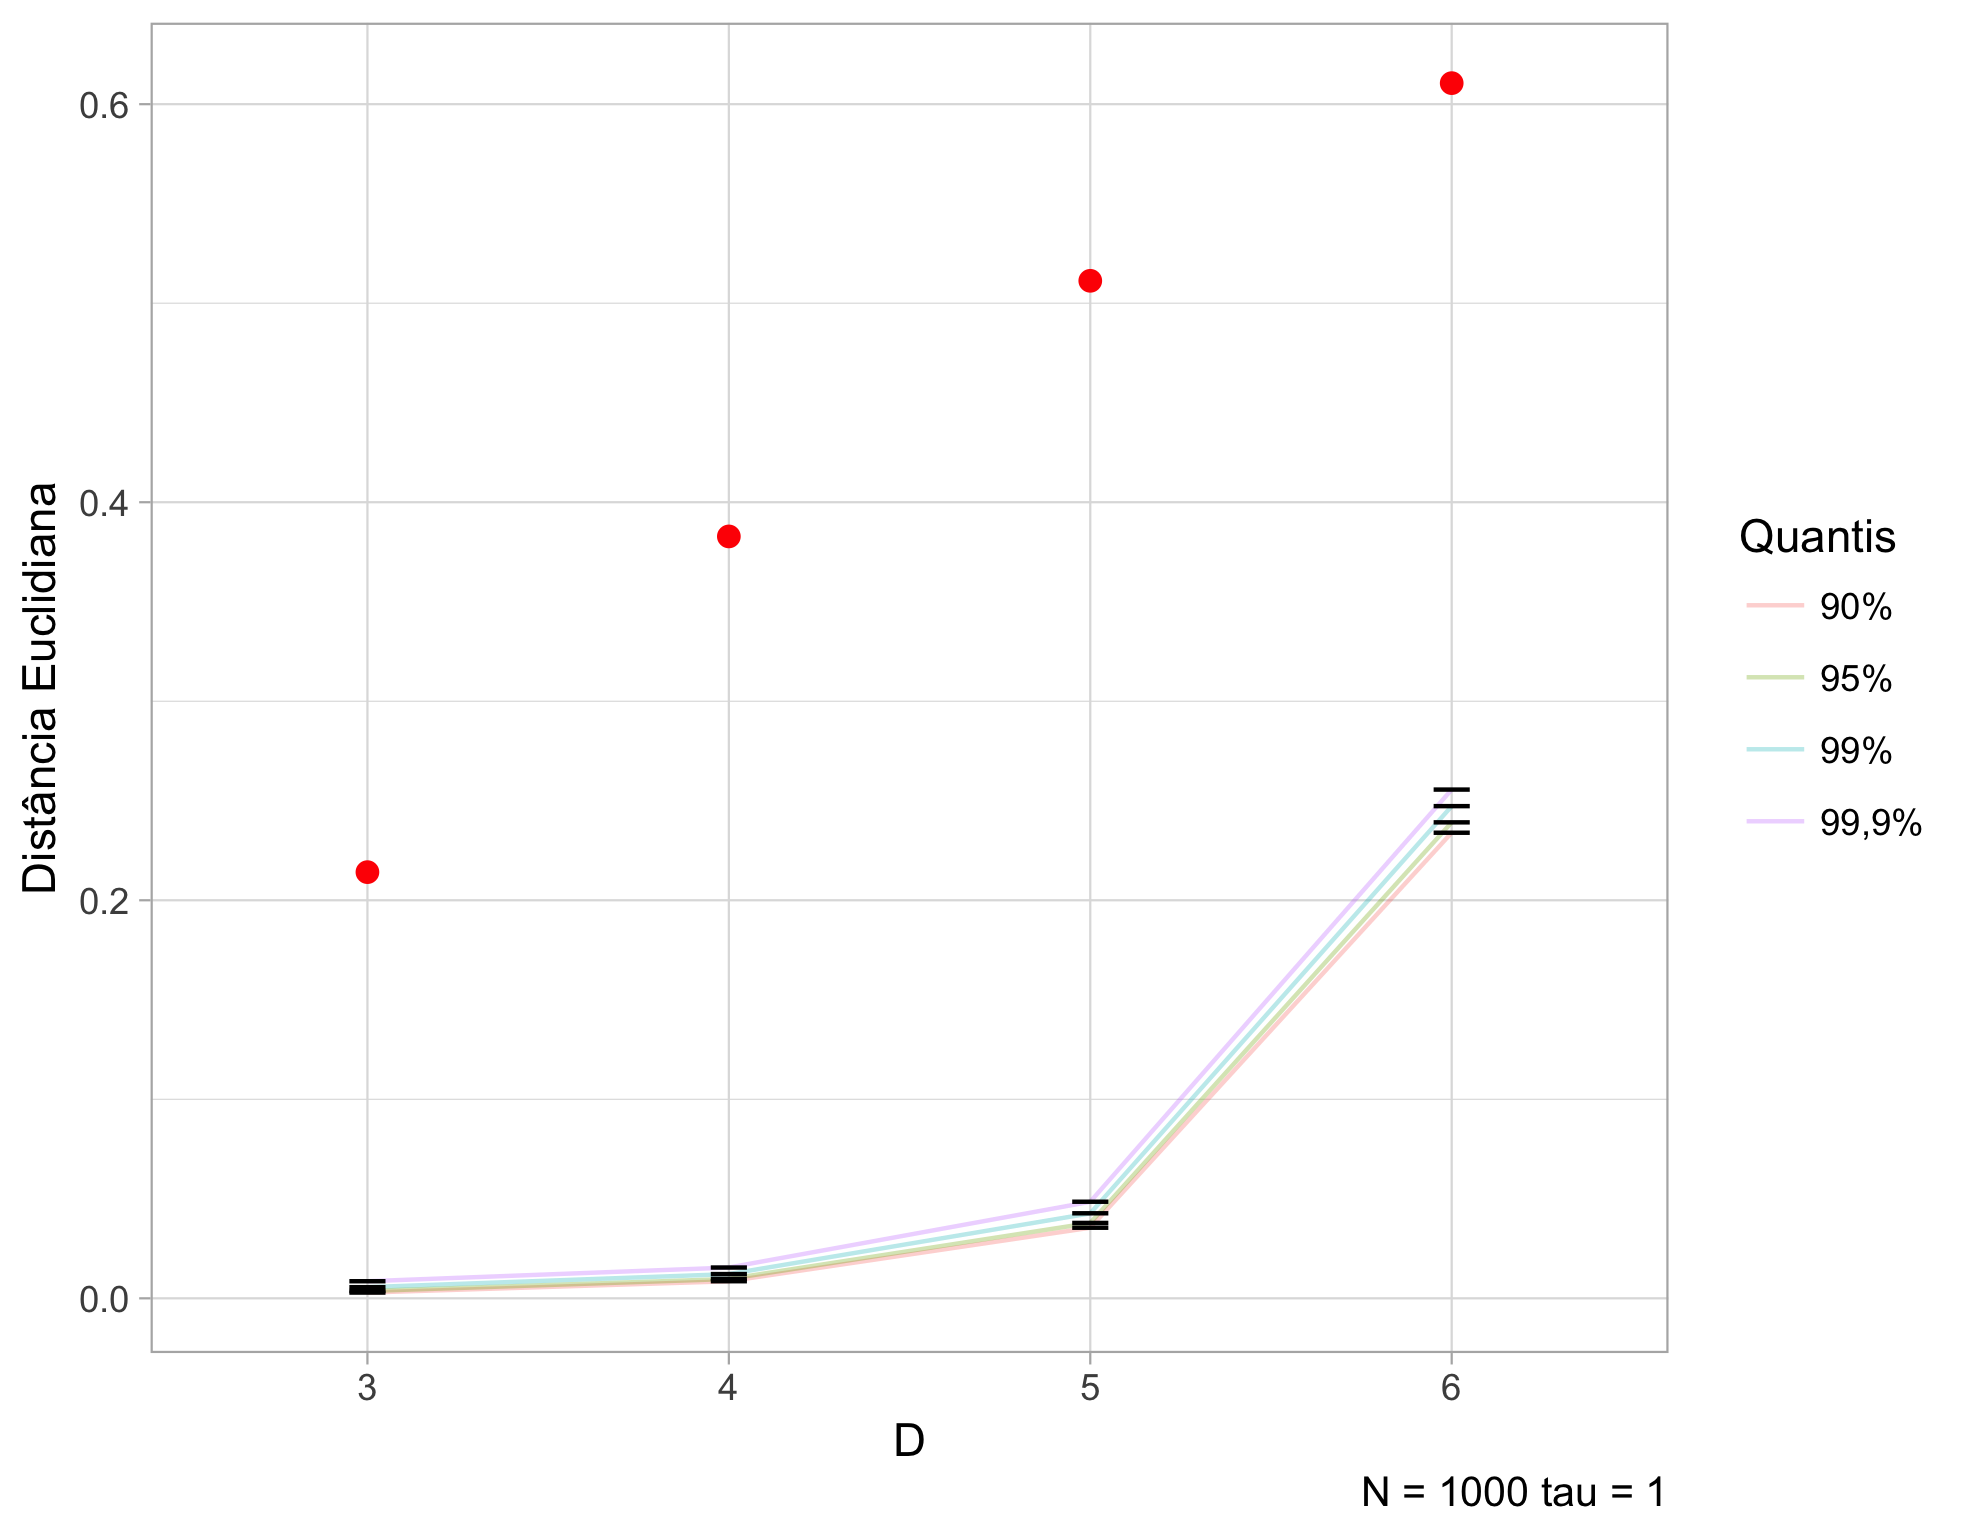
\includegraphics[width=.65\linewidth]{ConfidInt_mapa_logistico_1k_t1}
		\caption{Pontos característicos do mapa logístico e intervalos de confiança.}\label{Fig:ConfidInt_mapa_logistico_1k_t1}
	\end{figure}
	\end{block}
\end{frame}

%-------------------------------------------------------     
\section{Conclusão}
%-------------------------------------------------------

\begin{frame}{Conclusão}{}
	\begin{block}{Conclusão}
		Neste trabalho analisamos a possibilidade de a distância euclidiana de pontos no plano $(H\times C)$ de sequências ao ponto $(1,0)$, referência teórica de ruído branco, poderem ser usadas como uma estatística de teste para a hipótese de a sequência ser ruído branco.
		Verificamos que essa possibilidade existe, e que essa estatística é capaz de identificar, com limitações, o mapa logístico (que já foi usado como gerador de números pseudoaleatórios), movimento browniano e ruído com autocorrelação.
		Para este último, fizemos uma análise preliminar do poder do teste em função da intensidade da correlação.
	\end{block}
\end{frame}

\begin{frame}{Conclusão}{}
	\begin{block}{Conclusão}
	Verificamos, também, que os geradores Mersenne-Twister e Randu são considerados ruído branco, mesmo sendo eles técnicas algorítmicas de geração de observações pseudoaleatórias.
	\pause
	
	Uma limitação deste trabalho é que apenas verificamos a qualidade do gerador em relação a um de estrutura ideal.
	Com isso, limitamos a aplicabilidade do nosso trabalho à análise de séries que, potencialmente, são ocorrências de variáveis aleatórias independentes e identicamente distribuídas.	
	\end{block}
\end{frame}

\begin{frame}{Conclusão}{}
	\begin{block}{Conclusão}
	Há farta literatura que caracteriza diferentes tipos de estruturas como, por exemplo, processos estocásticos do tipo $f^{-k}$.
	A nossa metodologia pode, em princípio, ser aplicada a quaisquer processos mas, para isso, é necessário o conhecimento da distribuição dos padrões ordinais do processo de referência.
	No nosso caso, trata-se da lei uniforme sobre os padrões, que é característica de ruído branco.
	Não conhecemos resultados que caracterizem de forma teórica as leis de outros processos.
	\pause
	
	Há, contudo, uma solução para esse problema: estimar a lei característica do padrão de interesse.
	Isso pode ser feito através de estudos Monte Carlo, mas tal extensão foge ao objetivo deste trabalho.
	\end{block}
\end{frame}

\begin{frame}{Conclusão}{}
	\begin{block}{Conclusão}
		
	\end{block}
\end{frame}
% % % ACF Slide em branco

%-------------------------------------------------------     
\section{Referências Bibliográficas}
%-------------------------------------------------------
\begin{frame}[allowframebreaks]
	\frametitle{Referências}
%	\bibliographystyle{amsalpha}
%	\bibliographystyle{agsm_url}
	\bibliography{references}
\end{frame}

{\1
\begin{frame}[plain,noframenumbering]
  \finalpage{Obrigado}
\end{frame}}

\end{document}